\documentclass[a4paper,12pt]{article}
\usepackage{docsTemplate}
\usepackage{array}
\usepackage{longtable}
\usepackage{float}
\usepackage[official]{eurosym}
\usepackage{pgf-pie}
\usepackage{makecell}
\usepackage{xltabular}
\usepackage{amsmath}
\usepackage{caption}
\setcounter{secnumdepth}{4}
\setcounter{tocdepth}{4}
\setTitle{Specifica Tecnica}
\setAuthors{Mattia Oliva Medin \\ & Francesco Balestro \\ & Bianca Zaghetto \\ & Sara Gioia Fichera}
\setVerificators{Nenad Radulovic \\ & Filippo Compagno \\ & Francesco Balestro \\ & Bianca Zaghetto \\ & Sara Gioia Fichera \\ & Mattia Oliva Medin \\ & Andrea Masiero}
\setApprovation{Francesco Balestro}
\setVersion{1.0}
\setType{Esterno}
\setDestination{Team Three Technologies \\ & Prof. Tullio Vardanega \\ & Prof. Riccardo Cardin \\ & Sanmarco Informatica SpA}

\begin{document}
    \include{docTitlepage}

    \section*{Registro delle modifiche} {
        \begin{table}[h!]
            \rowcolors{2}{lightgray}{white}
                \begin{tabularx}{\textwidth}{|l|l|l|l|L|L|}
                \hline
                \textbf{Vers.} & \textbf{Data} & \textbf{Autore} & \textbf{Ruolo} & \textbf{Verifica} & \textbf{Oggetto} \\
                \hline
                \textbf{1.0} & 26/04/26 & Francesco Balestro & Responsabile &  & Approvazione documento \\
                \hline
                \textbf{0.9} & 26/04/26 & Mattia Oliva
                Medin & Programmatore & Filippo Compagno & Correzioni varie \\
                \hline
                \textbf{0.8} & 26/04/26 & Bianca Zaghetto & Verificatore & Nenad Radulovic & Aggiornamento requisiti e grafici \\
                \hline
                \textbf{0.7} & 26/04/26 & Francesco Balestro & Responsabile & Andrea Masiero & Stesura "Infrastructure layer" e "Classi per il rendering" \\
                \hline
                \textbf{0.6} & 26/04/26 & Sara Gioia Fichera & Programmatore & Mattia Oliva Medin & Stesura "Domain layer" e "Persistence layer" \\
                \hline
                \textbf{0.5} & 25/04/26 & Francesco Balestro & Responsabile & Bianca Zaghetto & Prima stesura "Design pattern", "Oggetti di trasferimento dati", "Presentation layer" e "Application layer" \\
                \hline
                \textbf{0.4} & 22/04/26 & Francesco Balestro & Responsabile & Sara Gioia Fichera & Prima stesura Architetture e aggiornamento sezione "Tecnologie" \\
                \hline
                \textbf{0.3} & 14/04/26 & Bianca Zaghetto & Programmatore & Francesco Balestro & Riferimenti normativi \\
                \hline
                \textbf{0.2} & 13/04/26 & Francesco Balestro & Verificatore & Filippo Compagno & Sezione "Scopo del documento" e "Tecnologie" \\
                \hline
                \textbf{0.1} & 11/04/26 & Mattia Oliva Medin & Programmatore & Nenad Radulovic & Prima stesura \\
                \hline
            \end{tabularx}
        \end{table}
    }
    \newpage
    
    \tableofcontents
    \newpage

    \listoffigures
    \newpage
    
    \listoftables
    \newpage

    \section{Introduzione} {
        \subsection{Scopo del documento} {        
            Il presente documento ha lo scopo di descrivere in maniera approfondita l’architettura del prodotto software, offrendo una rappresentazione chiara, organizzata e completa delle sue componenti, delle modalità con cui interagiscono e della loro distribuzione all’interno del sistema.\\
            \\
            La Specifica Tecnica costituisce un riferimento fondamentale per le attività di progettazione e sviluppo del prodotto, introducendo evoluzioni e miglioramenti volti a rafforzarne la solidità architetturale rispetto al PoC.\\
            \\
            In particolare, questo documento si propone di:
            \begin{itemize}
                \item Definire l’architettura logica del sistema, descrivendo le componenti principali, le rispettive responsabilità e le relazioni tra esse;
                \item Illustrare l’architettura di deployment, specificando come le diverse componenti vengono distribuite nell’ambiente di esecuzione;
                \item Presentare i design pattern architetturali adottati, mettendo in evidenza le scelte progettuali legate alle tecnologie utilizzate;
                \item Fornire ulteriori dettagli progettuali utili a valorizzare le decisioni architetturali e a facilitare la comprensione e la manutenzione del sistema.
            \end{itemize}
        }

        \subsection{Glossario} {
            Si rimanda al documento Glossario per chiarire i termini nel dominio del progetto che possono risultare ambigui o di difficile comprensione. I vocaboli presenti nel glossario sono stati segnalati seguendo la notazione:
            \begin{center}
                parola\textsubscript{G}
            \end{center}
        }
        
        \subsection{Riferimenti} {
            \subsubsection{Riferimenti normativi} {
                \begin{itemize}
                    \item \textit{Norme di progetto v2.0}
                    \begin{itemize}
                        \item \url{https://team-three-technologies.github.io/Documenti/2%20-%20PB/Documenti%20Interni/Norme_di_Progetto_v2_0.pdf}
                        \item[] (Ultimo accesso: 2026/04/11)
                    \end{itemize}
                    \item Capitolato C3
                    \begin{itemize}
                        \item \url{https://www.math.unipd.it/~tullio/IS-1/2025/Progetto/C3.pdf}
                        \item[] (Ultimo accesso: 2026/04/25)
                    \end{itemize}
                    \item Regolamento del Progetto Didattico
                    \begin{itemize}
                        \item \url{https://www.math.unipd.it/~tullio/IS-1/2025/Dispense/PD1.pdf}
                        \item[] (Ultimo accesso: 2026/04/05)
                    \end{itemize}
                \end{itemize}
            }
            \subsubsection{Riferimenti informativi} {
                \begin{itemize}
                    \item \textit{Glossario v1.0}
                    \begin{itemize}
                        \item \url{https://team-three-technologies.github.io/Documenti/2%20-%20PB/Documenti%20interni/Glossario_v1_0.pdf}
                        \item[] (Ultimo accesso: 2026/04/26)
                    \end{itemize}
                \end{itemize}
            }
        }
    }

    \section{Tecnologie} {
        Il progetto è stato realizzato adottando un insieme di tecnologie consolidate e complementari, selezionate per garantire semplicità di sviluppo, portabilità e facilità di manutenzione, in linea con un’architettura di tipo monolitico.\\
        \\
        La soluzione prevede un’applicazione desktop sviluppata utilizzando Angular per la gestione dell’interfaccia utente, integrata con Electron per la creazione del pacchetto eseguibile e per l’esecuzione in ambiente desktop. La comunicazione tra le componenti avviene tramite meccanismi di Inter-Process Communication (IPC) messi a disposizione da Electron, consentendo un’interazione strutturata ed efficiente tra le diverse parti dell’applicazione.\\
        \\
        Per la gestione della persistenza dei dati è stato adottato SQLite, scelto per la sua leggerezza, semplicità di integrazione e adeguatezza a contesti applicativi locali. In particolare, il database viene utilizzato per memorizzare e gestire i dati relativi al DIP, permettendone la consultazione e la visualizzazione all’interno dell’applicazione.\\
        \\
        Le tecnologie adottate sono state classificate in funzione del loro ruolo architetturale all’interno del sistema, includendo linguaggi di programmazione, framework per lo sviluppo dell’interfaccia utente, framework e runtime per l’esecuzione e il packaging dell’applicazione desktop, meccanismi di comunicazione tra componenti e sistemi di persistenza dei dati.\\
        \\
        Di seguito vengono descritte nel dettaglio le tecnologie adottate, evidenziandone le caratteristiche principali.

        \subsection{Linguaggi di programmazione}
        \begin{table}[H]
            \captionsetup{skip=10pt}
            \caption{Linguaggi di programmazione}
            \rowcolors{1}{lightgray}{white}
            \begin{tabular}{|>{\centering\arraybackslash}m{0.20\linewidth}|>{\centering\arraybackslash}m{0.10\linewidth}|>{\centering\arraybackslash}m{0.62\linewidth}|}
                \hline
                \textbf{Tecnologia} & \textbf{Versione} & \textbf{Descrizione} \\
                \hline
                \textbf{TypeScript} & 5.9.3 & TypeScript è un linguaggio di programmazione tipizzato basato su JavaScript, utilizzato per migliorare la qualità del codice grazie alla tipizzazione statica e al supporto per lo sviluppo di applicazioni scalabili e manutenibili. \\
                \hline
            \end{tabular}
        \end{table}

        \subsection{Framework per lo sviluppo dell'interfaccia utente}
        \begin{table}[H]
            \captionsetup{skip=10pt}
            \caption{Framework per lo sviluppo dell'interfaccia utente}
            \rowcolors{1}{lightgray}{white}
            \begin{tabular}{|>{\centering\arraybackslash}m{0.20\linewidth}|>{\centering\arraybackslash}m{0.10\linewidth}|>{\centering\arraybackslash}m{0.62\linewidth}|}
                \hline
                \textbf{Tecnologia} & \textbf{Versione} & \textbf{Descrizione} \\
                \hline
                \textbf{Angular} & 21.2.0 & Angular è un framework frontend basato su TypeScript, utilizzato per la realizzazione di applicazioni web strutturate e modulari tramite un’architettura a componenti. \\
                \hline
            \end{tabular}
        \end{table}

        \subsection{Framework e runtime di esecuzione desktop}
        \begin{table}[H]
            \captionsetup{skip=10pt}
            \caption{Framework e runtime di esecuzione desktop}
            \rowcolors{1}{lightgray}{white}
            \begin{tabular}{|>{\centering\arraybackslash}m{0.20\linewidth}|>{\centering\arraybackslash}m{0.10\linewidth}|>{\centering\arraybackslash}m{0.62\linewidth}|}
                \hline
                \textbf{Tecnologia} & \textbf{Versione} & \textbf{Descrizione} \\
                \hline
                \textbf{Electron} & 40.8.2 & Electron è un framework per lo sviluppo di applicazioni desktop multipiattaforma basato su tecnologie web, che integra un runtime basato su Chromium e Node.js e fornisce strumenti per il packaging e l’esecuzione dell’applicazione. \\
                \hline
            \end{tabular}
        \end{table}

        \subsection{Librerie}
        \begin{table}[H]
            \captionsetup{skip=10pt}
            \caption{Librerie}
            \rowcolors{1}{lightgray}{white}
            \begin{tabular}{|>{\centering\arraybackslash}m{0.20\linewidth}|>{\centering\arraybackslash}m{0.10\linewidth}|>{\centering\arraybackslash}m{0.62\linewidth}|}
                \hline
                \textbf{Tecnologia} & \textbf{Versione} & \textbf{Descrizione} \\
                \hline
                \textbf{better-sqlite3} & 12.6.2 & Libreria per Node.js che fornisce un’interfaccia sincrona ed efficiente per l’utilizzo di database SQLite, integrando direttamente il motore SQLite e semplificando l’esecuzione di query e la gestione dei dati. \\
                \hline
                \textbf{fast-xml-parser} & 5.5.9 & Libreria JavaScript veloce per il parsing e la conversione di file XML in oggetti JavaScript, e viceversa. \\
                \hline
                \textbf{tsyringe} & 4.10.0 & Libreria di dependency injection per TypeScript che facilita la gestione delle dipendenze e l’inversione del controllo. \\
                \hline
            \end{tabular}
        \end{table}

        \subsection{Strumenti di sviluppo}
        \begin{table}[H]
            \captionsetup{skip=10pt}
            \caption{Strumenti di sviluppo}
            \rowcolors{1}{lightgray}{white}
            \begin{tabular}{|>{\centering\arraybackslash}m{0.20\linewidth}|>{\centering\arraybackslash}m{0.10\linewidth}|>{\centering\arraybackslash}m{0.62\linewidth}|}
                \hline
                \textbf{Tecnologia} & \textbf{Versione} & \textbf{Descrizione} \\
                \hline
                \textbf{prettier} & 3.8.1 & Prettier è un formatter automatico di codice che garantisce uno stile consistente e leggibile in diversi linguaggi. \\
                \hline
                \textbf{electron-builder} & 26.8.1 & Strumento per il packaging e la distribuzione di applicazioni Electron in eseguibili per diverse piattaforme. \\
                \hline
            \end{tabular}
        \end{table}

        \subsection{Tecnologie per analisi dinamica}
        \begin{table}[H]
            \captionsetup{skip=10pt}
            \caption{Tecnologie per analisi dinamica}
            \rowcolors{1}{lightgray}{white}
            \begin{tabular}{|>{\centering\arraybackslash}m{0.20\linewidth}|>{\centering\arraybackslash}m{0.10\linewidth}|>{\centering\arraybackslash}m{0.62\linewidth}|}
                \hline
                \textbf{Tecnologia} & \textbf{Versione} & \textbf{Descrizione} \\
                \hline
                \textbf{vitest} & 4.0.8 & Vitest è un framework di testing veloce per progetti JavaScript/TypeScript, progettato per integrarsi con Vite e supportare test unitari e di integrazione. \\
                \hline
                \textbf{@vitest/coverage-v8} & 4.0.8 & @vitest/coverage-v8 è un plugin per Vitest che utilizza il motore V8 per generare report di code coverage durante l’esecuzione dei test. \\
                \hline
            \end{tabular}
        \end{table}
    }

    \section{Architettura} {
        \subsection{Architettura di deployment} {
            L’architettura di deployment del sistema è di tipo \textbf{monolitico}, in quanto l’applicazione viene distribuita come un’unica unità software autocontenuta. Tutte le componenti necessarie al funzionamento del sistema, incluse le dipendenze e le risorse applicative, sono incluse all’interno dello stesso pacchetto eseguibile.\\
            \\
            Questa scelta consente di semplificare il processo di installazione e configurazione per l’utente finale, eliminando la necessità di servizi esterni o di componenti distribuiti. L’applicazione può quindi essere eseguita in locale in modo indipendente, garantendo portabilità e coerenza dell’ambiente di esecuzione.\\
            \\
            Il packaging e la distribuzione dell’applicazione sono gestiti tramite \verb|electron-builder|, uno strumento specifico per applicazioni \textit{Electron}, che consente la creazione di eseguibili per le principali piattaforme desktop. Questo processo permette di ottenere un unico installer che incapsula l’intero sistema e tutte le sue dipendenze.
        }

        \subsection{Architettura logica} {
            La natura duale di Electron impone una distinzione architetturale fondamentale tra i due processi che compongono il sistema - il \textit{Main process} e il \textit{Renderer process} – ciascuno dei quali adotta un proprio stile architetturale in funzione delle proprie responsabilità.
            I due processi comunicano esclusivamente tramite il meccanismo di Inter-Process Communication (IPC) fornito da \textit{Electron}, che costituisce il confine architetturale tra le due componenti.
            L'unica parte di codice condivisa tra i due processi a livello di sorgente, non di runtime, sono i DTO (Data Transfer Objects), definiti nella cartella \verb|shared/| e descritti nella Sezione \ref{sec:DTO} (questi per convenienza espositiva sono trattati insieme al \textit{Main process}).
            Questa separazione è fondamentale per garantire sicurezza, prestazioni e manutenibilità del sistema di visualizzazione dei pacchetti DIP.
            
            \subsubsection{Architettura logica del Main process} {
                Il \textit{{Main process}} rappresenta il processo principale dell'applicazione \textit{Electron}. Ogni applicazione \textit{Electron} ha un unico \textit{Main process}, che viene eseguito all'avvio dell'applicazione e costituisce il punto di ingresso. Le sue caratteristiche principali sono:
                \begin{itemize}
                    \item \textbf{Accesso privilegiato}: il \textit{Main process} ha accesso completo alle API del sistema operativo e alle risorse native, inclusi file system, finestre di dialogo, processi shell e operazioni crittografiche;
                    \item \textbf{Gestione del ciclo di vita}: è responsabile della creazione e gestione delle finestre dell'applicazione (BrowserWindow) e del controllo del ciclo di vita complessivo dell'applicazione (avvio, chiusura, gestione degli eventi di sistema);
                    \item \textbf{Ospite della logica di business}: nel progetto, il \textit{Main process} ospita i layer applicativi più profondi: l'application layer (casi d'uso), il domain layer (entità e value object), il persistence layer (repository e accesso al database) e l'infrastructure layer (provider per file system, hashing, base64, dialoghi, shell);
                    \item \textbf{Accesso al database}: solo il \textit{Main process} interagisce direttamente con il database SQLite locale tramite \texttt{better-sqlite3}, garantendo l'integrità e la consistenza dei dati;
                    \item \textbf{Isolamento delle operazioni critiche}: tutte le operazioni che richiedono accesso al file system (lettura di file DIP, copia, esportazione), calcoli crittografici (hash, base64) e interazione con il sistema operativo (apertura di file, finestre di dialogo) sono eseguite esclusivamente nel Main process.
                \end{itemize}
                
                \noindent Nel contesto del progetto, il \textit{Main process} segue un'architettura \textbf{layered}, che organizza la logica applicativa in livelli distinti con responsabilità ben definite, al fine di garantire una chiara separazione delle competenze, una maggiore manutenibilità e una migliore scalabilità logica del sistema.\\
                In questo modello architetturale, ogni livello espone servizi ben definiti verso il livello superiore e interagisce esclusivamente con quelli adiacenti, riducendo l'accoppiamento tra le componenti.
                Questa struttura consente di isolare la logica applicativa e la gestione dei dati, facilitando l'evoluzione indipendente delle singole parti del sistema.\\\\
                La divisione è in cinque layer principali: presentation layer (lato main), application layer, domain layer, persistence layer e infrastructure layer, ciascuno con un ruolo ben definito all'interno del sistema.
                \begin{itemize}
                    \item \textbf{Presentation layer (lato main)}: costituisce il punto di ingresso delle richieste provenienti dal Renderer process.
                    È composto dagli handler IPC che ricevono le richieste dal Renderer process e le traducono in chiamate ai casi d'uso dell'application layer.
                    Svolge un ruolo analogo a quello di un controller in un'architettura MVC, disaccoppiando il meccanismo di comunicazione IPC dalla logica applicativa sottostante.
                    \item \textbf{Application layer}: contiene la logica applicativa e coordina le operazioni tra il presentation layer e l'accesso ai dati. 
                    Si occupa della gestione del flusso applicativo, dell'orchestrazione delle operazioni sul DIP (importazione, ricerca, verifica integrità, esportazione) e dell'implementazione dei casi d'uso (es. \texttt{AutoImportDipService}, \texttt{GetDipContentService}, \texttt{SearchDocumentsService}).
                    Questo layer dipende dalle interfacce dei repository (definite nel persistence layer), dalle entità del dominio (domain layer) e dai provider per operazioni specifiche (definite nell'infrastructure layer) applicando il principio di dependency inversion.
                    \item \textbf{Domain layer}: rappresenta il cuore del sistema, contenendo le entità di business e i value object che modellano i concetti fondamentali del dominio di conservazione digitale.
                    Questo layer è completamente indipendente dai dettagli infrastrutturali e non ha dipendenze verso layer esterni, incarnando il principio dell'\textit{Hexagonal Architecture} (core del dominio isolato).
                    \item \textbf{Persistence layer}: gestisce la persistenza e l'accesso ai dati contenuti nel pacchetto DIP.
                    Utilizza \verb|better-sqlite3| per l'interazione con il database locale, permettendo l'esecuzione di query sui metadati e la gestione strutturata delle informazioni archivistiche.
                    Implementa il pattern Repository (Sezione \ref{sec:Repository}), fornendo interfacce che astraggono completamente i dettagli implementativi del database.
                    Le implementazioni concrete dei repository risiedono in questo layer.
                    \item \textbf{Infrastructure layer}: fornisce servizi tecnici e infrastrutturali ai layer superiori.
                    Include provider per l'accesso al file system, per il calcolo di hash crittografici, per la decodifica base64, per la gestione di finestre di dialogo e per l'interazione con la shell del sistema operativo.
                    Questo layer implementa le interfacce definite nei layer superiori, seguendo il principio di dependency inversion.
                \end{itemize}

                \noindent La comunicazione tra i diversi layer segue un flusso controllato 
                dall'alto verso il basso:
                \begin{itemize}
                    \item Il \textbf{presentation layer (lato main)} riceve le richieste IPC dal Renderer process e le delega all'\textbf{application layer};
                    \item L'\textbf{application layer} orchestra le operazioni utilizzando le entità del \textbf{domain layer};
                    \item Per la persistenza, l'\textbf{application layer} utilizza le interfacce dei repository fornite dal \textbf{persistence layer};
                    \item Il \textbf{persistence layer} delega le operazioni tecniche (accesso al file system, calcoli crittografici) all'\textbf{infrastructure layer}.
                \end{itemize}

                \noindent Questa organizzazione a cinque layer garantisce una separazione netta delle responsabilità, facilitando la testabilità (ogni layer può essere testato in isolamento con mock dei layer inferiori), la manutenibilità (modifiche a un layer non influenzano gli altri) e l'evoluzione indipendente delle singole componenti del sistema.
            }
            
            \subsubsection{Architettura logica del Renderer process} {
                Il \textit{Renderer process} è il processo incaricato di eseguire l'interfaccia utente dell'applicazione. Ogni finestra (BrowserWindow) creata dal \textit{Main process} esegue il proprio \textit{Renderer process}, isolato dagli altri. Le sue caratteristiche principali sono:
                \begin{itemize}
                    \item \textbf{Ambiente sandboxed}: per ragioni di sicurezza, il \textit{Renderer process} opera in un ambiente limitato (\textit{sandbox}) con accesso ridotto alle risorse di sistema. Non può accedere direttamente al file system, al database o alle API native del sistema operativo;
                    \item \textbf{Hosting dell'interfaccia utente}: il \textit{Renderer process} esegue l'applicazione \textit{Angular}, che gestisce il rendering delle viste, l'interazione con l'utente e la presentazione dei dati;
                    \item \textbf{Comunicazione controllata}: per interagire con il \textit{Main process}, il \textit{Renderer process} utilizza esclusivamente il meccanismo di IPC (Inter-Process Communication) fornito da \textit{Electron}, attraverso il servizio \texttt{ElectronIPCService};
                    \item \textbf{Gestione dello stato reattivo}: utilizza i segnali (signals) di \textit{Angular} per mantenere uno stato reattivo e sincronizzato tra i vari componenti dell'interfaccia.
                \end{itemize}
                
                \noindent Nel contesto del progetto, il \textit{Renderer process} adotta il pattern architetturale \textbf{Model-View-ViewModel (MVVM)}, proprio del framework \textit{Angular}, che separa la logica di presentazione dalla visualizzazione e dalla gestione dei dati.
                Questa scelta è naturalmente imposta da Angular e risulta coerente con la responsabilità del Renderer process, che è esclusivamente quella di presentare i dati e raccogliere gli input dell'utente.\\
                \\
                Le tre componenti del pattern si mappano come segue:
                \begin{itemize}
                    \item \textbf{Model}: i dati ricevuti dal \textit{Main process} tramite IPC, rappresentati dai DTO definiti nella cartella \verb|shared/|.
                    Costituiscono la fonte di verità per la visualizzazione e non contengono alcuna logica applicativa.
                    \item \textbf{ViewModel}: i componenti container (es. \texttt{DipDashboardContainer}) e i servizi \textit{Angular} (es. \texttt{ElectronIPCService}), che orchestrano la logica di presentazione, gestiscono lo stato dell'applicazione tramite segnali (signals) di \textit{Angular} e mediano la comunicazione con il \textit{Main process} tramite IPC.
                    \item \textbf{View}: i componenti presentazionali (es. \texttt{DocumentListComponent}, \texttt{DocumentDetailsComponent}, \texttt{FiltersComponent}, \texttt{DocumentPreviewComponent}), responsabili esclusivamente della visualizzazione dei dati e della raccolta degli input utente, senza alcuna logica applicativa o di stato.
                \end{itemize}

                \noindent Il confine tra ViewModel e \textit{Main process} è attraversato esclusivamente tramite IPC: il ViewModel non conosce i dettagli implementativi del Main process, ma interagisce con esso attraverso il contratto definito dai DTO e dagli handler IPC.
            }
            
            \subsubsection{Comunicazione tra Main process e Renderer process}\label{sec:ipc-communication} {
                La comunicazione tra i due processi avviene tramite il meccanismo di Inter-Process Communication (IPC) fornito da \textit{Electron}, implementato nel progetto attraverso il servizio \texttt{ElectronIPCService} (Sezione \ref{par:ElectronIPCService}) nel \textit{Renderer process} e l'esposizione selettiva di API tramite \texttt{contextBridge} nel \textit{Main process}.\\
                \\
                Il modello di comunicazione adottato è asincrono basato su \texttt{Promise}: il \textit{Renderer process} invoca un metodo sul servizio \texttt{ElectronIPCService} (ad esempio \texttt{autoImport()}, \texttt{content()}, \texttt{searchDocuments()}) che, tramite IPC, richiede al \textit{Main process} di eseguire l'operazione corrispondente. Il \textit{Main process}, al completamento, restituisce una risposta standardizzata attraverso il DTO \texttt{IpcResponse<T>} (Sezione \ref{par:IpcResponse}), che incapsula sia i dati di successo che eventuali errori. Questo pattern garantisce una gestione uniforme degli errori e la tipizzazione forte delle risposte.\\
                \\
                La comunicazione segue il modello \textit{request-initiated}: sebbene sia sempre il \textit{Renderer process} a iniziare una richiesta, il \textit{Main process} può successivamente inviare notifiche asincrone (eventi di progresso o completamento) attraverso i canali IPC, a cui il \textit{Renderer process} può sottoscriversi tramite il metodo \texttt{on()} del servizio. Questo approccio è particolarmente utile per non bloccare il sistema con operazioni di lunga durata come il controllo dell'integrità del pacchetto.
            }
        }
        \subsection{Design pattern} {
            \subsubsection{Dependency injection} {
                \paragraph{Descrizione del pattern}\mbox{}\\
                Il pattern Dependency Injection è un design pattern che ha lo scopo di separare la creazione delle dipendenze dall’utilizzo delle stesse all’interno dei componenti di un sistema.\\
                \\
                In questo approccio, un oggetto non istanzia direttamente le proprie dipendenze, ma le riceve dall’esterno, tipicamente tramite il costruttore o metodi dedicati. Questo consente di definire in modo esplicito le relazioni tra i componenti, riducendo l’accoppiamento e migliorando l’organizzazione del codice.\\
                \\
                Le modalità principali attraverso cui può essere applicata la dependency injection sono:
                \begin{itemize}
                    \item Constructor Injection: le dipendenze vengono fornite al momento della creazione dell’oggetto;
                    \item Setter Injection: le dipendenze vengono assegnate successivamente tramite metodi setter.
                \end{itemize}
                
                \noindent Nel contesto del progetto è stato adottato l’approccio basato su Constructor Injection.
                
                \paragraph{Motivazioni dell’utilizzo del pattern}\mbox{}\\
                L’adozione del pattern Dependency Injection all’interno del progetto consente di ottenere diversi benefici:
                \begin{itemize}
                    \item \textbf{riduzione dell’accoppiamento}: i componenti non dipendono direttamente dalle implementazioni concrete delle loro dipendenze;
                    \item \textbf{flessibilità}: è possibile sostituire facilmente le implementazioni senza modificare il codice client;
                    \item \textbf{testabilità}: facilita l’utilizzo di oggetti simulati (mock) durante le fasi di test;
                    \item \textbf{modularità}: i componenti risultano più indipendenti e riutilizzabili;
                    \item \textbf{gestione semplificata delle dipendenze}: consente di delegare la creazione e l’iniezione delle dipendenze a componenti esterni o framework dedicati.
                \end{itemize}
                
                \paragraph{Utilizzo del pattern nel progetto}\mbox{}\\
                Nel progetto, il pattern Dependency Injection è stato adottato sia nel Main process che nel Renderer process, sfruttando approcci specifici per ciascun ambiente.\\
                \\
                Nel Main process (Node.js/Electron), la dependency injection è implementata manualmente tramite il passaggio esplicito delle dipendenze nei costruttori delle classi. Questo approccio, noto come \textit{constructor injection}, è stato utilizzato, per esempio, nei seguenti casi:
                \begin{itemize}
                    \item Ciascun servizio (ad esempio \texttt{LocalFileSystemProvider},\\ \texttt{CryptoHashProvider}, \texttt{DatabaseProvider}) riceve le proprie dipendenze (come\\ \texttt{AppConfig}) tramite costruttore;
                    \item Le classi che implementano i casi d'uso (come \texttt{AutoImportDipService}) ricevono repository, provider e mapper necessari attraverso il costruttore;
                    \item I repository (ad esempio \texttt{DipRepository}, \texttt{DocumentRepository}) ricevono l'istanza del database tramite dependency injection.
                \end{itemize}
                
                \noindent Nel Renderer process (Angular), la dependency injection è nativa del framework. Angular fornisce un sistema di dependency injection gerarchico che permette di:
                \begin{itemize}
                    \item Dichiarare i servizi (come \texttt{ElectronIPCService}) come \texttt{@Injectable()} e registrarli nei provider del modulo o del componente;
                    \item Iniettare automaticamente le dipendenze nei costruttori dei componenti Angular (ad esempio \texttt{DipDashboardContainer} riceve \texttt{ElectronIPCService} tramite costruttore);
                    \item Sfruttare il ciclo di vita dei servizi (singleton per l'intera applicazione o scoped per modulo/componente).
                \end{itemize}
                
                \noindent Questo approccio garantisce un basso accoppiamento tra le classi, facilitando la testabilità (attraverso il mocking delle dipendenze) e la manutenibilità del codice.
            }
            \subsubsection{Builder} {
                \paragraph{Descrizione del pattern}\mbox{}\\
                Il pattern Builder è un design pattern creazionale che consente di costruire oggetti complessi passo dopo passo, separando il processo di costruzione dalla rappresentazione finale dell’oggetto.\\
                \\
                Questo pattern risulta particolarmente utile quando un oggetto deve essere creato con numerosi parametri opzionali o con diverse configurazioni possibili. Il Builder fornisce un’interfaccia fluida per impostare le proprietà desiderate e costruire infine l’oggetto tramite un metodo dedicato.\\
                \\
                Il processo di costruzione avviene tipicamente attraverso una classe builder che espone metodi per impostare i vari attributi e un metodo finale (ad esempio build()) che restituisce l’oggetto completo.
                
                \paragraph{Motivazioni dell’utilizzo del pattern}\mbox{}\\
                L’utilizzo del pattern Builder nel progetto porta i seguenti vantaggi:
                \begin{itemize}
                    \item \textbf{leggibilità}: rende più chiaro il processo di creazione di oggetti complessi;
                    \item \textbf{flessibilità}: consente di creare diverse configurazioni dello stesso oggetto;
                    \item \textbf{immutabilità}: facilita la creazione di oggetti immutabili;
                    \item \textbf{controllo della costruzione}: permette di validare i dati prima della creazione dell’oggetto;
                    \item \textbf{riduzione dei costruttori}: evita la presenza di costruttori con un numero elevato di parametri.
                \end{itemize}
                
                \paragraph{Utilizzo del pattern nel progetto}\mbox{}\\
                Il pattern Builder è stato impiegato nel progetto per la costruzione dinamica di query di ricerca sui metadati dei documenti. Data la natura variabile e composizionale dei criteri di ricerca (l'utente può specificare un numero arbitrario di filtri di diverso tipo), il pattern Builder permette di costruire progressivamente la stringa contenente la query di ricerca con tutte le condizioni specificate nella richiesta.\\
                \\
                Nello specifico, il componente \texttt{SQLiteDocumentRepository} (Sezione \ref{par:SQLiteDocumentRepository}) agisce come \textit{Director} che, a partire dai filtri selezionati dall'utente ricevuti nella richiesta, costruisce la query aggiungendo il filtri con il metodo \texttt{withFilter}. La costruzione avviene in modo incrementale.\\
                \\
                Nel codice il pattern è implementato mediante l'uso di metodi come \texttt{withFilter()} e \texttt{buildQuery()}, che servono rispettivamente per aggiungere un filtro e per ottenere il risultato.
            }
            \subsubsection{Strategy} {
                \paragraph{Descrizione del pattern}\mbox{}\\
                Il pattern Strategy è un design pattern comportamentale che consente di definire una famiglia di algoritmi, incapsularli e renderli intercambiabili.\\
                \\
                Il pattern permette di selezionare dinamicamente l’algoritmo da utilizzare a runtime, senza modificare il codice client. Ogni algoritmo viene implementato in una classe separata che implementa una comune interfaccia.\\
                \\
                Il contesto mantiene un riferimento a una strategia e delega ad essa l’esecuzione del comportamento, permettendo così di cambiare comportamento in modo dinamico.
                
                \paragraph{Motivazioni dell’utilizzo del pattern}\mbox{}\\
                L’utilizzo del pattern Strategy nel progetto offre diversi vantaggi:
                \begin{itemize}
                    \item \textbf{flessibilità}: consente di cambiare comportamento dinamicamente;
                    \item \textbf{estendibilità}: è possibile aggiungere nuove strategie senza modificare il codice esistente;
                    \item \textbf{riusabilità}: gli algoritmi sono isolati e riutilizzabili;
                    \item \textbf{eliminazione di strutture condizionali complesse}: riduce l’uso di if o switch;
                    \item \textbf{separazione delle responsabilità}: il codice risulta più organizzato e manutenibile.
                \end{itemize}
                
                \paragraph{Utilizzo del pattern nel progetto}\mbox{}\\
                Il pattern Strategy è stato utilizzato nel progetto per gestire le diverse versioni del formato dei pacchetti DIP durante l'attività di parsing. Poiché il formato DIP potrebbe evolvere nel tempo (ad esempio dalla versione 1 alla versione 2), è necessario poter supportare più versioni contemporaneamente senza modificare il codice esistente.\\
                \\
                Il pattern è implementato attraverso le seguenti interfacce e implementazioni:
                \begin{itemize}
                    \item \textbf{Strategy interfaces}: \texttt{DipIndexParser} (Sezione \ref{par:DipIndexParser}), \texttt{AipInfoParser} (Sezione \ref{par:AipInfoParser}), \texttt{DocumentMetadataParser} (Sezione \ref{par:DocumentMetadataParser}) definiscono il contratto per il parsing di specifiche componenti del pacchetto DIP;
                    \item \textbf{Concrete strategies}: \texttt{DipIndexParserV1} (Sezione \ref{par:DipIndexParserV1}), \texttt{AipInfoParserV1} (Sezione \ref{par:AipInfoParserV1}), \texttt{DocumentMetadataParserV1} (Sezione \ref{par:DocumentMetadataParserV1}) implementano la logica di parsing per la versione 1 del formato;
                    \item \textbf{Context}: \texttt{DipParserV1} (Sezione \ref{par:DipParserV1}) agisce come contesto, ricevendo le strategie specifiche tramite dependency injection e delegando a esse le operazioni di parsing.
                \end{itemize}
                
                \noindent In futuro, per supportare una nuova versione del formato (ad esempio versione 2), sarà sufficiente:
                \begin{enumerate}
                    \item Creare nuove classi \texttt{DipIndexParserV2}, \texttt{AipInfoParserV2}, \texttt{DocumentMetadataParserV2} che implementano le rispettive interfacce;
                    \item Creare un nuovo contesto \texttt{DipParserV2} che utilizza le nuove strategie;
                    \item Modificare la configurazione della dependency injection per selezionare la versione appropriata in base a un rilevatore automatico del formato.
                \end{enumerate}
                
                \noindent L'adozione del pattern Strategy, permette di aderire all'Open/Closed Principle (principio di apertura/chiusura) del SOLID: il sistema è aperto all'estensione (nuove versioni del formato) ma chiuso alla modifica delle classi esistenti.
            }
            \subsubsection{Repository}\label{sec:Repository} {
                \paragraph{Descrizione del pattern}\mbox{}\\
                Il pattern Repository è un design pattern che fornisce un’astrazione per l’accesso ai dati, separando la logica di business dalla logica di persistenza.\\
                \\
                Il repository agisce come un intermediario tra il dominio dell’applicazione e la sorgente dei dati (database, file system, servizi esterni), offrendo metodi per eseguire operazioni di lettura e scrittura senza esporre i dettagli implementativi.\\
                \\
                In questo modo, il resto dell’applicazione può interagire con i dati tramite un’interfaccia uniforme, indipendentemente dalla tecnologia di persistenza utilizzata.
                
                \paragraph{Motivazioni dell’utilizzo del pattern}\mbox{}\\
                L’utilizzo del pattern Repository nel progetto comporta diversi benefici:
                \begin{itemize}
                    \item \textbf{separazione delle responsabilità}: la logica di accesso ai dati è isolata dalla logica applicativa;
                    \item \textbf{manutenibilità}: eventuali modifiche al sistema di persistenza non impattano il resto del codice;
                    \item \textbf{testabilità}: è possibile utilizzare mock dei repository nei test;
                    \item \textbf{astrazione}: il sistema non dipende da una specifica tecnologia di storage;
                    \item \textbf{organizzazione del codice}: centralizza le operazioni di accesso ai dati in componenti dedicati.
                \end{itemize}
                
                \paragraph{Utilizzo del pattern nel progetto}\mbox{}\\
                Il pattern Repository è stato adottato nel Main process per mediare l'accesso ai dati persistenti, astraendo completamente i dettagli implementativi del database sottostante (SQLite) e fornendo un'interfaccia simile a una collezione per l'accesso agli oggetti di dominio.\\
                \\
                Le principali componenti del pattern sono:
                \begin{itemize}
                    \item \textbf{Repository interfaces}: interfacce come \texttt{DipRepository}, \texttt{DocumentRepository},\\ \texttt{DocumentClassRepository}, \texttt{ConservationProcessRepository} definiscono le operazioni di persistenza disponibili (ad esempio \texttt{findById()}, \texttt{save()}, \texttt{findAll()}, \texttt{delete()});
                    \item \textbf{Concrete repositories}: implementazioni concrete di queste interfacce (ad esempio \texttt{DipRepositoryImpl}) che utilizzano l'istanza del database fornita da \texttt{DatabaseProvider} (Sezione \ref{par:DatabaseProvider}) per eseguire le effettive operazioni SQL;
                    \item \textbf{Use case}: i casi d'uso (come \texttt{AutoImportDipService}) dipendono dalle interfacce dei repository, non dalle implementazioni concrete, applicando il principio di dependency inversion.
                \end{itemize}
                
                \noindent Ad esempio, durante l'importazione automatica di un pacchetto DIP, \texttt{AutoImportDipService} utilizza:
                \begin{itemize}
                    \item \texttt{DipRepository} per salvare le informazioni del pacchetto DIP;
                    \item \texttt{DocumentRepository} per salvare i documenti e i loro allegati;
                    \item \texttt{DocumentClassRepository} per salvare le classi documentali;
                    \item \texttt{ConservationProcessRepository} per salvare i processi di conservazione.
                \end{itemize}
            }
        }

        \subsection{Main process - Dettagli implementativi} {
            \begin{figure}[H]
                \centering
                
\includegraphics[
                    angle=90,
                    width=\textheight,
                    height=\textwidth,
                    keepaspectratio
                ]{class_diagrams/main.pdf}
                \caption{UML Main process}
            \end{figure}
            \subsubsection{Oggetti di trasferimento dati (DTO)}\label{sec:DTO} {
                Per implementare i DTO sono state utilizzate le \verb|interface| di TypeScript, che sono uno strumento di tipizzazione statica utilizzato per descrivere la forma di un oggetto (attributi, metodi, tipi), presente solo in fase di compilazione per il controllo dei tipi; non esistono a runtime e non impongono realmente un'implementazione come nei linguaggi OOP classici. Sono in questo caso utili solo a verificare che una struttura rispetti la forma dichiarata. Sono rappresentate nei nostri diagrammi UML come una classe con attributi pubblici.  
                \paragraph{IpcResponse$<$T$>$}\label{par:IpcResponse}\mbox{}\\
                \begin{figure}[H]
                    \centering
                    
\includegraphics[width=0.2\textwidth]{class_diagrams/ipc-response.pdf}
                    \caption{UML IpcResponse$<$T$>$}
                \end{figure}
                \noindent Rappresenta un DTO generico che funge da wrapper per la risposta di comunicazione tra processi (IPC) nel sistema. Questo oggetto è utilizzato nella presentation logic per trasportare in modo uniforme il risultato di un'operazione, contenendo sia i dati di successo che eventuali errori.\\
                \\
                \textbf{Descrizione degli attributi della struttura}:
                \begin{itemize}
                    \item \textbf{data: T $|$ null}: rappresenta i dati di tipo T restituiti dall'operazione in caso di successo; assume valore \texttt{null} in caso di errore;
                    \item \textbf{error: string $|$ null}: rappresenta il messaggio di errore associato all'operazione in caso di fallimento; assume valore \texttt{null} in caso di successo.
                \end{itemize}
                
                \paragraph{DipRequestDTO}\label{par:DipRequestDTO}\mbox{}\\
                \begin{figure}[H]
                    \centering
                    
\includegraphics[width=0.2\textwidth]{class_diagrams/dip-request-dto.pdf}
                    \caption{UML DipRequestDTO}
                \end{figure}
                \noindent Rappresenta un DTO (Data Transfer Object) per la richiesta di operazioni su un pacchetto DIP. Questo oggetto è utilizzato nella presentation logic per trasportare l'identificativo del pacchetto DIP su cui eseguire le operazioni richieste.\\
                \\
                \textbf{Descrizione degli attributi della struttura}:
                \begin{itemize}
                    \item \textbf{dipUuid: string}: rappresenta l'identificativo univoco del pacchetto DIP su cui eseguire l'operazione richiesta.
                \end{itemize}
                \paragraph{AutoImportDipResponseDTO}\label{par:AutoImportDipResponseDTO}\mbox{}\\
                \begin{figure}[H]
                    \centering
                    
\includegraphics[width=0.3\textwidth]{class_diagrams/autoimport-response-dto.pdf}
                    \caption{UML AutoImportDipResponseDTO}
                \end{figure}
                \noindent Rappresenta un DTO per la risposta all'operazione di importazione automatica di un pacchetto DIP. Questo oggetto è utilizzato nella presentation logic per restituire l'identificativo del pacchetto DIP che è stato importato.\\
                \\
                \textbf{Descrizione degli attributi della struttura}:
                \begin{itemize}
                    \item \textbf{dipUuid: string}: rappresenta l'identificativo univoco del pacchetto DIP che è stato importato automaticamente nel sistema.
                \end{itemize}
                \paragraph{DipContentResponseDTO}\label{par:DipContentResponseDTO}\mbox{}\\
                \begin{figure}[H]
                    \centering
                    
\includegraphics[width=0.4\textwidth]{class_diagrams/dip-content-response-dto.pdf}
                    \caption{UML DipContentResponseDTO}
                \end{figure}
                \noindent Rappresenta un DTO per la risposta all'operazione di recupero del contenuto di un pacchetto DIP. Questo oggetto è utilizzato nella presentation logic per restituire le informazioni principali del pacchetto DIP e l'elenco dei documenti in esso contenuti.\\
                \\
                \textbf{Descrizione degli attributi della struttura}:
                \begin{itemize}
                    \item \textbf{uuid: string}: rappresenta l'identificativo univoco del pacchetto DIP;
                    \item \textbf{creationDate: Date}: rappresenta la data di creazione del pacchetto DIP;
                    \item \textbf{documentNumber: number}: rappresenta il numero totale di documenti contenuti nel pacchetto DIP;
                    \item \textbf{aipNumber: number}: rappresenta il numero di pacchetti AIP (Archival Information Package) associati o aggregati nel DIP;
                    \item \textbf{documentsList: DocumentEssentialsDTO[0..*]}: rappresenta una lista opzionale di oggetti DocumentEssentialsDTO contenenti le informazioni essenziali dei documenti presenti nel pacchetto DIP.
                \end{itemize}

                \paragraph{FileIntegrityDTO}\label{par:FileIntegrityDTO}\mbox{}\\
                \begin{figure}[H]
                    \centering
                    
\includegraphics[width=0.2\textwidth]{class_diagrams/file-integrity-dto.pdf}
                    \caption{UML FileIntegrityDTO}
                \end{figure}
                \noindent Rappresenta un DTO per la verifica dell'integrità di un file all'interno del DIP. Questo oggetto è utilizzato nella presentation logic per riportare l'esito del controllo di integrità su un singolo file.\\
                \\
                \textbf{Descrizione degli attributi della struttura}:
                \begin{itemize}
                    \item \textbf{uuid: string}: rappresenta l'identificativo univoco del file sottoposto a verifica di integrità;
                    \item \textbf{status: boolean}: rappresenta l'esito della verifica di integrità del file; assume valore \texttt{true} se il file è integro, \texttt{false} altrimenti.
                \end{itemize}
                \paragraph{DocumentIntegrityResponseDTO}\label{par:DocumentIntegrityResponseDTO}\mbox{}\\
                \begin{figure}[H]
                    \centering
                    
\includegraphics[width=0.3\textwidth]{class_diagrams/document-integrity-dto.pdf}
                    \caption{UML DocumentIntegrityResponseDTO}
                \end{figure}
                \noindent Rappresenta un DTO per la verifica dell'integrità di un documento all'interno del DIP. Questo oggetto è utilizzato nella presentation logic per riportare l'esito del controllo di integrità sul file principale del documento e sugli eventuali allegati.\\
                \\
                \textbf{Descrizione degli attributi della struttura}:
                \begin{itemize}
                    \item \textbf{integrity: FileIntegrityDTO}: rappresenta l'esito della verifica di integrità del file principale del documento;
                    \item \textbf{attachments: FileIntegrityDTO[0..*]}: rappresenta una lista opzionale di oggetti FileIntegrityDTO contenenti gli esiti della verifica di integrità per ciascun allegato associato al documento.
                \end{itemize}
                \paragraph{DocumentEssentialsAttachmentDTO}\label{par:DocumentEssentialsAttachmentDTO}\mbox{}\\
                \begin{figure}[H]
                    \centering
                    
\includegraphics[width=0.3\textwidth]{class_diagrams/attachment-essentials-dto.pdf}
                    \caption{UML DocumentEssentialsAttachmentDTO}
                \end{figure}
                \noindent Rappresenta un DTO per le informazioni essenziali di un allegato all'interno di un documento nel DIP. Questo oggetto è utilizzato nella presentation logic per trasportare i dati minimi di un allegato, come l'identificativo e il nome.\\
                \\
                \textbf{Descrizione degli attributi della struttura}:
                \begin{itemize}
                    \item \textbf{uuid: string}: rappresenta l'identificativo univoco dell'allegato;
                    \item \textbf{name: string}: rappresenta il nome dell'allegato.
                \end{itemize}
                \paragraph{DocumentEssentialsDTO}\label{par:DocumentEssentialsDTO}\mbox{}\\
                \begin{figure}[H]
                    \centering
                    
\includegraphics[width=0.5\textwidth]{class_diagrams/document-essentials-dto.pdf}
                    \caption{UML DocumentEssentialsDTO}
                \end{figure}
                \noindent Rappresenta un DTO per le informazioni essenziali di un documento nel DIP. Questo oggetto è utilizzato nella presentation logic per trasportare i dati minimi di un documento, come l'identificativo, il nome e la lista degli allegati associati.\\
                \\
                \textbf{Descrizione degli attributi della struttura}:
                \begin{itemize}
                    \item \textbf{documentuuid: string}: rappresenta l'identificativo univoco del documento;
                    \item \textbf{documentName: string}: rappresenta il nome del documento;
                    \item \textbf{documentAttachments: DocumentEssentialsAttachmentDTO[0..*]}: rappresenta una lista opzionale di oggetti DocumentEssentialsAttachmentDTO contenente le informazioni essenziali degli allegati associati al documento.
                \end{itemize}

                \paragraph{SearchResponseDTO}\label{par:SearchResponseDTO}\mbox{}\\
                \begin{figure}[H]
                    \centering
                    
\includegraphics[width=0.3\textwidth]{class_diagrams/search-response-dto.pdf}
                    \caption{UML SearchResponseDTO}
                \end{figure}
                \noindent Rappresenta un DTO per la risposta all'operazione di ricerca di documenti nel DIP. Questo oggetto è utilizzato nella presentation logic per restituire l'elenco dei documenti che soddisfano i criteri di ricerca specificati.\\
                \\
                \textbf{Descrizione degli attributi della struttura}:
                \begin{itemize}
                    \item \textbf{results: DocumentEssentialsDTO[0..*]}: rappresenta una lista opzionale di oggetti DocumentEssentialsDTO contenente le informazioni essenziali dei documenti trovati in seguito all'esecuzione della ricerca.
                \end{itemize}

                \paragraph{SearchFilterDTO}\label{par:SearchFilterDTO}\mbox{}\\
                \begin{figure}[H]
                    \centering
                    
\includegraphics[width=0.2\textwidth]{class_diagrams/search-filter-dto.pdf}
                    \caption{UML SearchFilterDTO}
                \end{figure}
                \noindent Rappresenta un DTO per la definizione di un filtro di ricerca nel DIP. Questo oggetto è utilizzato nella presentation logic per specificare un criterio di ricerca basato su una coppia tipo-valore applicabile ai metadati dei documenti.\\
                \\
                \textbf{Descrizione degli attributi della struttura}:
                \begin{itemize}
                    \item \textbf{type: string}: rappresenta il tipo di metadato su cui applicare il filtro di ricerca (es. autore, data, titolo);
                    \item \textbf{value: string}: rappresenta il valore da confrontare con il metadato specificato per il filtro di ricerca.
                \end{itemize}

                \paragraph{SearchRequestDTO}\label{par:SearchRequestDTO}\mbox{}\\
                \begin{figure}[H]
                    \centering
                    
\includegraphics[width=0.3\textwidth]{class_diagrams/search-request-dto.pdf}
                    \caption{UML SearchRequestDTO}
                \end{figure}
                \noindent Rappresenta un DTO per la richiesta di ricerca di documenti nel DIP. Questo oggetto è utilizzato nella presentation logic per trasportare l'insieme dei filtri da applicare nella ricerca sui metadati dei documenti.\\
                \\
                \textbf{Descrizione degli attributi della struttura}:
                \begin{itemize}
                    \item \textbf{filters: SearchFilterDTO[0..*]}: rappresenta una lista opzionale di oggetti SearchFilterDTO contenente i filtri da applicare per la ricerca dei documenti.
                \end{itemize}
                \paragraph{AttachmentResponseDTO}\label{par:AttachmentResponseDTO}\mbox{}\\
                \begin{figure}[H]
                    \centering
                    
\includegraphics[width=0.3\textwidth]{class_diagrams/attachment-response-dto.pdf}
                    \caption{UML AttachmentResponseDTO}
                \end{figure}
                \noindent Rappresenta un DTO per la risposta contenente le informazioni di un allegato di un allegato nel DIP. Questo oggetto è utilizzato nella presentation logic per trasportare i dati di un allegato, inclusi l'identificativo, il percorso e l'estensione del file.\\
                \\
                \textbf{Descrizione degli attributi della struttura}:
                \begin{itemize}
                    \item \textbf{uuid: string}: rappresenta l'identificativo univoco dell'allegato;
                    \item \textbf{path: string}: rappresenta il percorso del file allegato all'interno del sistema;
                    \item \textbf{extension: string}: rappresenta l'estensione del file allegato.
                \end{itemize}
                \paragraph{SubjectDTO}\label{par:SubjectDTO}\mbox{}\\
                \begin{figure}[H]
                    \centering
                    
\includegraphics[width=0.1\textwidth]{class_diagrams/subject-dto.pdf}
                    \caption{UML SubjectDTO}
                \end{figure}
                \noindent Rappresenta un DTO per la risposta contenente le informazioni di un soggetto coinvolto nella conservazione di un documento contenuto nel DIP. Questo oggetto è utilizzato nella presentation logic per trasportare i dati di un allegato, inclusi l'identificativo, il percorso e l'estensione del file.\\
                \\
                \textbf{Descrizione degli attributi della struttura}:
                \begin{itemize}
                    \item \textbf{id: number}: rappresenta l'identificativo univoco del soggetto;
                    \item \textbf{role: string}: rappresenta il ruolo con qui il soggetto ha interagito con il documento;
                    \item \textbf{name: string}: rappresenta le informazioni utili a identificare il soggetto;
                    \item \textbf{type: string}: rappresenta il tipo del soggetto.
                \end{itemize}
                \paragraph{DocumentDetailsResponseDTO}\label{par:DocumentDetailsResponseDTO}\mbox{}\\
                \begin{figure}[H]
                    \centering
                    
\includegraphics[width=0.3\textwidth]{class_diagrams/document-details-response-dto.pdf}
                    \caption{UML DocumentDetailsResponseDTO}
                \end{figure}
                \noindent Rappresenta un DTO per la risposta all'operazione di recupero dei dettagli di un documento nel DIP. Questo oggetto è utilizzato nella presentation logic per restituire tutte le informazioni relative a un documento, inclusi metadati, contenuto, dimensioni e allegati.\\
                \\
                \textbf{Descrizione degli attributi della struttura}:
                \begin{itemize}
                    \item \textbf{uuid: string}: rappresenta l'identificativo univoco del documento;
                    \item \textbf{name: string}: rappresenta il nome del documento;
                    \item \textbf{extension: string}: rappresenta l'estensione del file principale del documento;
                    \item \textbf{registrationType: string}: rappresenta il tipo di registrazione del documento;
                    \item \textbf{registrationDate: string}: rappresenta la data di registrazione del documento;
                    \item \textbf{registrationTime: string}: rappresenta l'orario di registrazione del documento;
                    \item \textbf{content: string}: rappresenta l'oggetto del documento;
                    \item \textbf{version: string}: rappresenta il numero di versione del documento;
                    \item \textbf{filesCount: number}: rappresenta il numero totale di file associati al documento;
                    \item \textbf{totalSize: string}: rappresenta la dimensione complessiva del documento e dei suoi allegati;
                    \item \textbf{attachmentsCount: number}: rappresenta il numero di allegati associati al documento;
                    \item \textbf{attachments: AttachmentResponseDTO[0..*]}: rappresenta una lista opzionale di oggetti AttachmentResponseDTO contenente le informazioni dettagliate degli allegati del documento.
                    \item \textbf{documentType: string}: rappresenta la tipologia documentale del documento;
                    \item \textbf{documentNumber: string}: rapresenta il numero ;
                    \item \textbf{registryCode: string}: rappresenta il codice di registro del documento;
                    \item \textbf{aggregationType: string}: rappresenta il tipo di aggregazione del documento;
                    \item \textbf{subjects: SubjectDTO[0..*]}: rappresenta la lista dei soggeti dei soggetti che hanno interagito con il documento.
                \end{itemize}

                \paragraph{DocumentRequestDTO}\label{par:DocumentRequestDTO}\mbox{}\\
                \begin{figure}[H]
                    \centering
                    
\includegraphics[width=0.2\textwidth]{class_diagrams/document-request-dto.pdf}
                    \caption{UML DocumentRequestDTO}
                \end{figure}
                \noindent Rappresenta un DTO per la richiesta di operazioni su un documento nel DIP. Questo oggetto è utilizzato nella presentation logic per trasportare l'identificativo del documento su cui eseguire l'operazione richiesta.\\
                \\
                \textbf{Descrizione degli attributi della struttura}:
                \begin{itemize}
                    \item \textbf{documentUuid: string}: rappresenta l'identificativo univoco del documento su cui eseguire l'operazione richiesta.
                \end{itemize}

                \paragraph{FileRequestDTO}\label{par:FileRequestDTO}\mbox{}\\
                \begin{figure}[H]
                    \centering
                    
\includegraphics[width=0.2\textwidth]{class_diagrams/file-request-dto.pdf}
                    \caption{UML FileRequestDTO}
                \end{figure}
                \noindent Rappresenta un DTO per la richiesta di operazioni su un file all'interno di un documento nel DIP. Questo oggetto è utilizzato nella presentation logic per trasportare l'identificativo del documento e l'identificativo opzionale del file su cui eseguire l'operazione richiesta.\\
                \\
                \textbf{Descrizione degli attributi della struttura}:
                \begin{itemize}
                    \item \textbf{documentUuid: string}: rappresenta l'identificativo univoco del documento contenente il file;
                    \item \textbf{fileUuid: string $|$ undefined}: rappresenta l'identificativo univoco del file su cui eseguire l'operazione; se non specificato (undefined), l'operazione viene eseguita sul file principale del documento.
                \end{itemize}
                \paragraph{FileInternalPreviewResponseDTO}\label{par:FileInternalPreviewResponseDTO}\mbox{}\\
                \begin{figure}[H]
                    \centering
                    
\includegraphics[width=0.3\textwidth]{class_diagrams/file-int-preview-response-dto.pdf}
                    \caption{UML FileInternalPreviewResponseDTO}
                \end{figure}
                \noindent Rappresenta un DTO per la risposta all'operazione di generazione di un'anteprima interna di un file nel DIP. Questo oggetto è utilizzato nella presentation logic per restituire lo url con custom protocol generato per la visualizzazione all'interno dell'applicazione.\\
                \\
                \textbf{Descrizione degli attributi della struttura}:
                \begin{itemize}
                    \item \textbf{fileUrl: string}: rappresenta lo url con custom protocolo per l'anteprima interna del file, accessibile dall'applicazione per la visualizzazione del contenuto.
                \end{itemize}
                \paragraph{ExportFileResponseDTO}\label{par:ExportFileResponseDTO}\mbox{}\\
                \begin{figure}[H]
                    \centering
                    
\includegraphics[width=0.2\textwidth]{class_diagrams/export-file-response-dto.pdf}
                    \caption{UML ExportFileResponseDTO}
                \end{figure}
                \noindent Rappresenta un DTO per la risposta all'operazione di esportazione di un file nel DIP. Questo oggetto è utilizzato nella presentation logic per restituire il percorso del file esportato sul file system locale.\\
                \\
                \textbf{Descrizione degli attributi della struttura}:
                \begin{itemize}
                    \item \textbf{path: string}: rappresenta il percorso del file esportato, indicando la posizione in cui il file è stato salvato sul file system.
                \end{itemize}
            }
            
            \subsubsection{Presentation layer}\label{sec:Presentation-layer} {
                \paragraph{DipHandler}\label{par:DipHandler}\mbox{}\\
                \begin{figure}[H]
                    \centering
                    
\includegraphics[width=0.7\textwidth]{class_diagrams/dip-handler.pdf}
                    \caption{UML DipHandler}
                \end{figure}
                \noindent Il DipHandler gestisce la Presentation Logic per la gestione dei pacchetti DIP. Coordina le operazioni di importazione automatica, recupero del contenuto e verifica dell'integrità dei pacchetti DIP.\\
                \\
                \textbf{Descrizione degli attributi della classe}:
                \begin{itemize}
                    \item \textbf{autoImportDipUseCase: AutoImportDipUseCase}: rappresenta il caso d'uso per l'importazione automatica dei pacchetti DIP; vedere la Sezione \ref{par:AutoImportDipUseCase};
                    \item \textbf{getDipContentUseCase: GetDipContentUseCase}: rappresenta il caso d'uso per il recupero del contenuto di un pacchetto DIP; vedere la Sezione \ref{par:GetDipContentUseCase};
                    \item \textbf{checkDipIntegrityUseCase: CheckDipIntegrityUseCase}: rappresenta il caso d'uso per la verifica dell'integrità di un pacchetto DIP; vedere la Sezione \ref{par:CheckDipIntegrityUseCase}.
                \end{itemize}
                
                \noindent \textbf{Descrizione dei metodi invocabili dalla classe}:
                \begin{itemize}
                    \item \textbf{DipHandler(autoImportDipUseCase: AutoImportDipUseCase,\\ getDipContentUseCase: GetDipContentUseCase,\\ checkDipIntegrityUseCase: CheckDipIntegrityUseCase)}:\\ costruttore della classe. Inizializza gli attributi autoImportDipUseCase, getDipContentUseCase e checkDipIntegrityUseCase con i valori passati come parametri;
                    \item \textbf{autoImport(): Promise$<$lpcResponse$<$AutoImportDipResponseDTO$>>$}: avvia il processo di importazione automatica dei pacchetti DIP disponibili nel sistema. Delega l'operazione al caso d'uso autoImportDipUseCase. Ritorna una Promise contenente la risposta con l'esito dell'importazione;
                    \item \textbf{getDipContent(dipRequestDto: DipRequestDTO):\\ Promise$<$lpcResponse$<$DipContentResponseDTO$>>$}: recupera il contenuto completo del pacchetto DIP specificato nel DTO. Delega l'operazione al caso d'uso getDipContentUseCase. Ritorna una Promise contenente la risposta con i dati del pacchetto;
                    \item \textbf{checkDipIntegrity(event: IpcMainEvent, dipRequestDto: DipRequestDTO):\\ Promise$<$void$>$}: verifica l'integrità del pacchetto DIP specificato, controllando checksum e firme digitali. Delega l'operazione al caso d'uso checkDipIntegrityUseCase. Genera eventi che rappresentano la disponibilità di un risultato, la fine dell'operazione o eventuali errori.
                \end{itemize}

                \paragraph{DocumentHandler}\label{par:DocumentHandler}\mbox{}\\
                \begin{figure}[H]
                    \centering
                    
\includegraphics[width=\textwidth]{class_diagrams/document-handler.pdf}
                    \caption{UML DocumentHandler}
                \end{figure}
                \noindent Il DocumentHandler gestisce l'Application Logic per la gestione dei documenti all'interno dei pacchetti DIP. Coordina le operazioni di visualizzazione dei dettagli, ricerca basata su metadati, anteprime interne ed esterne dei file, ed esportazione dei documenti.\\
                \\
                \textbf{Descrizione degli attributi della classe}:
                \begin{itemize}
                    \item \textbf{getDocumentDetailsUseCase: GetDocumentDetailsUseCase}: rappresenta il caso d'uso per il recupero dei dettagli di un documento; vedere la Sezione \ref{par:GetDocumentDetailsUseCase};
                    \item \textbf{searchDocumentsFromMetadataUseCase:\\ SearchDocumentsFromMetadataUseCase}: rappresenta il caso d'uso per la ricerca di documenti basata su metadati; vedere la Sezione \ref{par:SearchDocumentsFromMetadataUseCase};
                    \item \textbf{fileInternalPreviewUseCase: FileInternalPreviewUseCase}: rappresenta il caso d'uso per la generazione di anteprime interne dei file; vedere la Sezione \ref{par:FileInternalPreviewUseCase};
                    \item \textbf{fileExternalPreviewUseCase: FileExternalPreviewUseCase}: rappresenta il caso d'uso per la generazione di anteprime esterne dei file; vedere la Sezione \ref{par:FileExternalPreviewUseCase};
                    \item \textbf{exportDocumentUseCase: ExportFileUseCase}: rappresenta il caso d'uso per l'esportazione dei file; vedere la Sezione \ref{par:ExportFileUseCase}.
                \end{itemize}
            
            \noindent \textbf{Descrizione dei metodi invocabili dalla classe}:
                \begin{itemize}
                    \item \textbf{DocumentHandler(getDocumentDetailsUseCase:\\ GetDocumentDetailsUseCase, searchDocumentsFromMetadataUseCase:\\ SearchDocumentsFromMetadataUseCase, fileInternalPreviewUseCase:\\ FileInternalPreviewUseCase, fileExternalPreviewUseCase:\\ FileExternalPreviewUseCase, exportDocumentUseCase:\\ ExportFileUseCase)}: costruttore della classe. Inizializza gli attributi getDocumentDetailsUseCase, searchDocumentsFromMetadataUseCase, fileInternalPreviewUseCase, fileExternalPreviewUseCase e exportDocumentUseCase con i valori passati come parametri;
                    \item \textbf{getDocumentDetails(documentRequestDto: DocumentRequestDTO):\\ Promise$<$lpcResponse$<$DocumentDetailsResponseDTO$>>$}: recupera i dettagli del documento specificato nel DTO, inclusi metadati e informazioni strutturali. Delega l'operazione al caso d'uso getDocumentDetailsUseCase. Ritorna una Promise contenente la risposta con i dettagli del documento;
                    \item \textbf{searchDocuments(searchRequestDto: SearchRequestDTO):\\ Promise$<$lpcResponse$<$SearchResponseDTO$>>$}: esegue una ricerca di documenti basata sui criteri espressi nel DTO, interrogando i metadati indicizzati. Delega l'operazione al caso d'uso searchDocumentsFromMetadataUseCase. Ritorna una Promise contenente la risposta con i risultati della ricerca;
                    \item \textbf{fileInternalPreview(fileRequestDto: FileRequestDTO):\\ Promise$<$lpcResponse$<$FileInternalPreviewResponseDTO$>>$}: genera un'anteprima interna del file specificato, ottimizzata per la visualizzazione nell'applicazione. Delega l'operazione al caso d'uso fileInternalPreviewUseCase. Ritorna una Promise contenente la risposta con l'anteprima generata;
                    \item \textbf{fileExternalPreview(fileRequestDto: FileRequestDTO):\\ Promise$<$lpcResponse$<$ExportFileResponseDTO$>>$}: genera un'anteprima esterna del file specificato, producendo un URL o un contenuto condivisibile. Delega l'operazione al caso d'uso fileExternalPreviewUseCase. Ritorna una Promise contenente la risposta con i dati per l'anteprima esterna;
                    \item \textbf{exportFile(exportFileRequestDto: ExportFileRequestDTO):\\ Promise$<$lpcResponse$<$ExportFileResponseDTO$>>$}: esporta il file specificato nel formato richiesto. Delega l'operazione al caso d'uso exportDocumentUseCase. Ritorna una Promise contenente la risposta con il percorso del file esportato sul file system locale.
                \end{itemize}
            }
            
            \subsubsection{Application layer}\label{sec:Application-layer} {
                \paragraph{AutoImportDipUseCase}\label{par:AutoImportDipUseCase}\mbox{}\\
                \begin{figure}[H]
                    \centering
                    
\includegraphics[width=0.4\textwidth]{class_diagrams/auto-import-dip-uc.pdf}
                    \caption{UML AutoImportDipUseCase}
                \end{figure}
                \noindent L'interfaccia AutoImportDipUseCase definisce il contratto per il caso d'uso di importazione automatica dei pacchetti DIP nel sistema.\\
                \\
                \noindent \textbf{Descrizione dei metodi dell'interfaccia}:
                \begin{itemize}
                    \item \textbf{execute(): Promise$<$AutoImportDipResponseDTO$>$}: esegue l'operazione di importazione automatica dei pacchetti DIP disponibili nel sistema. Ritorna una Promise contenente la risposta con l’identificativo del pacchetto DIP che è stato importato. Si veda Sezione \ref{par:AutoImportDipResponseDTO}
                \end{itemize}
                \paragraph{AutoImportDipService}\label{par:AutoImportDipService}\mbox{}\\
                \begin{figure}[H]
                    \centering
                    
\includegraphics[width=\textwidth]{class_diagrams/auto-import-dip-service.pdf}
                    \caption{UML AutoImportDipService}
                \end{figure}
                \noindent La classe AutoImportDipService implementa l'interfaccia AutoImportDipUseCase, gestendo la logica applicativa per l'importazione automatica dei pacchetti DIP. Coordina l'accesso al file system, il parsing dei pacchetti, il mapping delle entità e la persistenza nei repository.\\
                \\
                \textbf{Descrizione degli attributi della classe}:
                \begin{itemize}
                    \item \textbf{BATCH\_SIZE: number = 50}: rappresenta la dimensione del batch di salvataggio dei documenti, cioè quanti documenti verranno costruiti prima di effettuare un salvataggio nel database;
                    \item \textbf{fileSystemProvider: FileSystemProvider}: rappresenta il provider per l'accesso al file system; vedere la Sezione \ref{par:FileSystemProvider};
                    \item \textbf{dipParser: DipParser}: rappresenta il parser per la decodifica dei pacchetti DIP; vedere la Sezione \ref{par:DipParser};
                    \item \textbf{dipMapper: DipMapper}: rappresenta il mapper per la trasformazione delle entità DIP; vedere la Sezione \ref{par:DipMapper};
                    \item \textbf{documentClassMapper: DocumentClassMapper}: rappresenta il mapper per le classi documentali; vedere la Sezione \ref{par:DocumentClassMapper};
                    \item \textbf{conservationProcessMapper: ConservationProcessMapper}: rappresenta il mapper per i processi di conservazione; vedere la Sezione \ref{par:ConservationProcessMapper};
                    \item \textbf{documentMapper: DocumentMapper}: rappresenta il mapper per i documenti; vedere la Sezione \ref{par:DocumentMapper};
                    \item \textbf{dipRepository: DipRepository}: rappresenta il repository per l'accesso ai dati dei pacchetti DIP; vedere la Sezione \ref{par:DipRepository};
                    \item \textbf{documentClassRepository: DocumentClassRepository}: rappresenta il repository per l'accesso ai dati delle classi documentali; vedere la Sezione \ref{par:DocumentClassRepository};
                    \item \textbf{conservationProcessRepository: ConservationProcessRepository}: rappresenta il repository per l'accesso ai dati dei processi di conservazione; vedere la Sezione \ref{par:ConservationProcessRepository};
                    \item \textbf{documentRepository: DocumentRepository}: rappresenta il repository per l'accesso ai dati dei documenti; vedere la Sezione \ref{par:DocumentRepository} 
                \end{itemize}
                
              \noindent \textbf{Descrizione dei metodi invocabili dalla classe}:
                \begin{itemize}
                    \item \textbf{AutoImportDipService(fileSystemProvider: FileSystemProvider, dipParser: DipParser, dipMapper: DipMapper, documentClassMapper:\\ DocumentClassMapper, conservationProcessMapper:\\ ConservationProcessMapper, dipRepository: DipRepository,\\ documentClassRepository: DocumentClassRepository, conservationProcessRepository: ConservationProcessRepository, documentRepository:\\ DocumentRepository)}: costruttore della classe. Inizializza tutti gli attributi con i valori passati come parametri;
                    \item \textbf{execute(): Promise$<$AutoImportDipResponseDTO$>$}: implementa il metodo dell'interfaccia. Esegue la scansione del file system tramite fileSystemProvider per individuare nuovi pacchetti DIP. Per ciascun pacchetto, utilizza dipParser per decodificare il contenuto, dipMapper e gli altri mapper per trasformare le entità, e infine persiste i dati nei repository corrispondenti. Ritorna una Promise contenente la risposta con l’identificativo del pacchetto DIP che è stato importato.
                \end{itemize}
                \paragraph{GetDipContentUseCase}\label{par:GetDipContentUseCase}\mbox{}\\
                \begin{figure}[H]
                    \centering
                    
\includegraphics[width=0.5\textwidth]{class_diagrams/get-dip-content-uc.pdf}
                    \caption{UML GetDipContentUseCase}
                \end{figure}
                \noindent L'interfaccia GetDipContentUseCase definisce il contratto per il caso d'uso di recupero del contenuto di un pacchetto DIP.\\
                \\
              \noindent \textbf{Descrizione dei metodi dell'interfaccia}:
                \begin{itemize}
                    \item \textbf{execute(dipUuid: string): Promise$<$DipContentResponseDTO$>$}: esegue l'operazione di recupero del contenuto del pacchetto DIP identificato dall'UUID specificato. Ritorna una Promise contenente la risposta con le informazioni principali del pacchetto DIP e l’elenco dei documenti in esso contenuti.
                \end{itemize}
                \paragraph{GetDipContentService}\label{par:GetDipContentService}\mbox{}\\
                \begin{figure}[H]
                    \centering
                    
\includegraphics[width=0.5\textwidth]{class_diagrams/get-dip-content-service.pdf}
                    \caption{UML GetDipContentService}
                \end{figure}
                \noindent La classe GetDipContentService implementa l'interfaccia GetDipContentUseCase, gestendo la logica applicativa per il recupero del contenuto di un pacchetto DIP. Coordina l'accesso ai repository per ottenere i metadati del pacchetto e dei documenti associati.\\
                \\
                \textbf{Descrizione degli attributi della classe}:
                \begin{itemize}
                    \item \textbf{dipRepository: DipRepository}: rappresenta il repository per l'accesso ai dati dei pacchetti DIP; vedere la Sezione \ref{par:DipRepository};
                    \item \textbf{documentRepository: DocumentRepository}: rappresenta il repository per l'accesso ai dati dei documenti; vedere la Sezione \ref{par:DocumentRepository}.
                \end{itemize}
                
              \noindent \textbf{Descrizione dei metodi invocabili dalla classe}:
                \begin{itemize}
                    \item \textbf{GetDipContentService(dipRepository: DipRepository, documentRepository: DocumentRepository)}: costruttore della classe. Inizializza gli attributi dipRepository e documentRepository con i valori passati come parametri;
                    \item \textbf{execute(dipUuid: string): Promise$<$DipContentResponseDTO$>$}: implementa il metodo dell'interfaccia. Recupera le informazioni del pacchetto DIP tramite dipRepository utilizzando l'UUID fornito. Successivamente, recupera i documenti associati al pacchetto tramite documentRepository. Compone e ritorna una Promise contenente la risposta con i dati principali del pacchetto DIP.
                \end{itemize}
                \paragraph{CheckDipIntegrityUseCase}\label{par:CheckDipIntegrityUseCase}\mbox{}\\
                \begin{figure}[H]
                    \centering
                    
\includegraphics[width=0.5\textwidth]{class_diagrams/check-integrity-uc.pdf}
                    \caption{UML CheckDipIntegrityUseCase}
                \end{figure}
                \noindent L'interfaccia CheckDipIntegrityUseCase definisce il contratto per il caso d'uso di verifica dell'integrità di un pacchetto DIP.\\
                \\
              \noindent \textbf{Descrizione dei metodi dell'interfaccia}:
                \begin{itemize}
                    \item \textbf{execute(dipUuid: string): AsyncGenerator$<$DocumentIntegrityResponseDTO$>$}: esegue l'operazione di verifica dell'integrità del pacchetto DIP identificato dall'UUID specificato. Controlla la consistenza dei file rispetto ai checksum registrati. Ritorna in maniera asincrona i risultati della verifica.
                \end{itemize}
                \paragraph{CheckDipIntegrityService}\label{par:CheckDipIntegrityService}\mbox{}\\
                \begin{figure}[H]
                    \centering
                    
\includegraphics[width=0.7\textwidth]{class_diagrams/check-integrity-service.pdf}
                    \caption{UML CheckDipIntegrityUseCase}
                \end{figure}
                \noindent La classe CheckDipIntegrityService implementa l'interfaccia CheckDipIntegrityUseCase, gestendo la logica applicativa per la verifica dell'integrità dei pacchetti DIP. Coordina l'accesso al file system, la decodifica dei contenuti in base64 e il calcolo degli hash per confrontarli con i valori di riferimento.\\
                \\
                \textbf{Descrizione degli attributi della classe}:
                \begin{itemize}
                    \item \textbf{documentRepository: DocumentRepository}: rappresenta il repository per l'accesso ai dati dei documenti; vedere la Sezione \ref{par:DocumentRepository};
                    \item \textbf{fileSystemProvider: FileSystemProvider}: rappresenta il provider per l'accesso al file system; vedere la Sezione \ref{par:FileSystemProvider};
                    \item \textbf{base64Provider: Base64Provider}: rappresenta il provider per la codifica/decodifica in base64; vedere la Sezione \ref{par:Base64Provider};
                    \item \textbf{hashProvider: HashProvider}: rappresenta il provider per il calcolo di hash crittografici; vedere la Sezione \ref{par:HashProvider}.
                \end{itemize}
                
              \noindent \textbf{Descrizione dei metodi invocabili dalla classe}:
                \begin{itemize}
                    \item \textbf{CheckDipIntegrityService(documentRepository: DocumentRepository, fileSystemProvider: FileSystemProvider, base64Provider: Base64Provider, hashProvider: HashProvider)}: costruttore della classe. Inizializza tutti gli attributi con i valori passati come parametri;
                    \item \textbf{computeFileHash(document: Document, file: File, trace: string \textbar null, algorithm: string \textbar null): Promise$<$boolean$>$}: metodo privato che calcola l'hash di un file specifico utilizzando il fileSystemProvider per accedere al file, il base64Provider per decodificare il contenuto e il hashProvider per eseguire il calcolo dell'hash. Ritorna una Promise che risolve a \texttt{true} se l'hash calcolato corrisponde a quello di riferimento, \texttt{false} altrimenti.
                    \item \textbf{execute(dipUuid: string): AsyncGenerator$<$DocumentIntegrityResponseDTO$>$}: implementa il metodo dell'interfaccia. Recupera i documenti contenuti nel DIP con relativi metadati, tra cui i checksum di riferimento, tramite documentRepository. Utilizza il metodo computeFileHash. Ritorna in maniera asincrona i risultati della verifica di un documento (file principale e allegati) uno per uno, in modo da poter essere chiamata in background senza bloccare il resto del sistema.
                \end{itemize}

                \paragraph{DeleteDipUseCase}\label{par:DeleteDipUseCase}\mbox{}\\
                \begin{figure}[H]
                    \centering
                    
\includegraphics[width=0.4\textwidth]{class_diagrams/delete-dip-uc.pdf}
                    \caption{UML DeleteDipUseCase}
                \end{figure}
                \noindent L'interfaccia DeleteDipUseCase definisce il contratto per l'eliminazione di un Dip e tutte le relative informazioni dal database.\\
                \\
              \noindent \textbf{Descrizione dei metodi dell'interfaccia}:
                \begin{itemize}
                    \item \textbf{execute(dipUuid: string): Promise$<$void$>$}: esegue l'operazione di eliminazione del Dip dal database.
                \end{itemize}
                \paragraph{DeleteDipService}\label{par:DeleteDipService}\mbox{}\\
                \begin{figure}[H]
                    \centering
                    
\includegraphics[width=0.3\textwidth]{class_diagrams/delete-dip-service.pdf}
                    \caption{UML DeleteDipService}
                \end{figure}
                \noindent La classe DeleteDipService implementa l'interfaccia DeleteDipUseCase, gestendo la logica applicativa per la cancellazione dal database di un pacchetto DIP. Coordina l'accesso al repository.\\
                \\
                \textbf{Descrizione degli attributi della classe}:
                \begin{itemize}
                    \item \textbf{dipRepository: DipRepository}: rappresenta il repository per l'accesso ai dati dei dip; vedere la Sezione \ref{par:DipRepository};
                \end{itemize}
                
              \noindent \textbf{Descrizione dei metodi invocabili dalla classe}:
                \begin{itemize}
                    \item \textbf{DeleteDipService(dipRepository: DipRepository)}: costruttore della classe. Inizializza tutti gli attributi con i valori passati come parametri;
                    \item \textbf{execute(dipUuid: string): Promise$<$void$>$}: implementa il metodo dell'interfaccia. Richiama il metodo di cancellazione del Dip nel repository passando lo UUID.
                \end{itemize}

                \paragraph{GetDocumentDetailsUseCase}\label{par:GetDocumentDetailsUseCase}\mbox{}\\
                \begin{figure}[H]
                    \centering
                    
\includegraphics[width=0.5\textwidth]{class_diagrams/get-doc-details-uc.pdf}
                    \caption{UML GetDocumentDetailsUseCase}
                \end{figure}
                \noindent L'interfaccia GetDocumentDetailsUseCase definisce il contratto per il caso d'uso di recupero dei dettagli di un documento all'interno del DIP.\\
                \\
              \noindent \textbf{Descrizione dei metodi dell'interfaccia}:
                \begin{itemize}
                    \item \textbf{execute(documentUuid: string): Promise$<$DocumentDetailsResponseDTO$>$}: esegue l'operazione di recupero dei dettagli del documento identificato dall'UUID specificato. Ritorna una Promise contenente la risposta con i dettagli del documento.
                \end{itemize}
                \paragraph{GetDocumentDetailsService}\label{par:GetDocumentDetailsService}\mbox{}\\
                \begin{figure}[H]
                    \centering
                    
\includegraphics[width=0.5\textwidth]{class_diagrams/get-doc-details-service.pdf}
                    \caption{UML GetDocumentDetailsService}
                \end{figure}
                \noindent La classe GetDocumentDetailsService implementa l'interfaccia GetDocumentDetailsUseCase, gestendo la logica applicativa per il recupero dei dettagli di un documento. Coordina l'accesso al repository per ottenere le informazioni del documento.\\
                \\
                \textbf{Descrizione degli attributi della classe}:
                \begin{itemize}
                    \item \textbf{documentRepository: DocumentRepository}: rappresenta il repository per l'accesso ai dati dei documenti; vedere la Sezione \ref{par:DocumentRepository}.
                \end{itemize}
                
              \noindent \textbf{Descrizione dei metodi invocabili dalla classe}:
                \begin{itemize}
                    \item \textbf{GetDocumentDetailsService(documentRepository: DocumentRepository)}: costruttore della classe. Inizializza l'attributo documentRepository con il valore passato come parametro;
                    \item \textbf{execute(documentUuid: string): Promise$<$DocumentDetailsResponseDTO$>$}: implementa il metodo dell'interfaccia. Recupera le informazioni del documento tramite documentRepository utilizzando l'UUID fornito. Compone e ritorna una Promise contenente la risposta con i dettagli completi del documento.
                    \item \textbf{unwrapSubject(subject: Record$<$string, string$>$, index: number):\\ SubjectDTO}: estrae le informazione del soggetto dai metadati relativi che gli vengono passate, dipende dallo schema dei metadati attuale.
                \end{itemize}
                \paragraph{SearchDocumentsFromMetadataUseCase}\label{par:SearchDocumentsFromMetadataUseCase}\mbox{}\\
                \begin{figure}[H]
                    \centering
                    
\includegraphics[width=0.6\textwidth]{class_diagrams/search-metadata-uc.pdf}
                    \caption{UML SearchDocumentsFromMetadataUseCase}
                \end{figure}
                \noindent L'interfaccia SearchDocumentsFromMetadataUseCase definisce il contratto per il caso d'uso di ricerca di documenti basata su metadati all'interno del DIP.\\
                \\
              \noindent \textbf{Descrizione dei metodi dell'interfaccia}:
                \begin{itemize}
                    \item \textbf{execute(filters: \{ type: string; value: string \}[0..*]):\\ Promise$<$SearchResponseDTO$>$}: esegue l'operazione di ricerca dei documenti applicando i filtri specificati sui metadati. I filtri sono espressi come array di oggetti contenenti il tipo di metadato da cercare e il valore da confrontare. Ritorna una Promise contenente la risposta con l'elenco dei documenti che soddisfano i criteri di ricerca. Vedere la Sezione \ref{par:SearchResponseDTO}
                \end{itemize}
                \paragraph{SearchDocumentsFromMetadataService}\label{par:SearchDocumentsFromMetadataService}\mbox{}\\
                \begin{figure}[H]
                    \centering
                    
\includegraphics[width=0.5\textwidth]{class_diagrams/search-metadata-service.pdf}
                    \caption{UML SearchDocumentsFromMetadataService}
                \end{figure}
                \noindent La classe SearchDocumentsFromMetadataService implementa l'interfaccia SearchDocumentsFromMetadataUseCase, gestendo la logica applicativa per la ricerca di documenti basata su metadati. Coordina l'accesso al repository per interrogare i documenti secondo i filtri forniti.\\
                \\
                \textbf{Descrizione degli attributi della classe}:
                \begin{itemize}
                    \item \textbf{documentRepository: DocumentRepository}: rappresenta il repository per l'accesso ai dati dei documenti; vedere la Sezione \ref{par:DocumentRepository}.
                \end{itemize}
                
              \noindent \textbf{Descrizione dei metodi invocabili dalla classe}:
                \begin{itemize}
                    \item \textbf{SearchDocumentsFromMetadataService(documentRepository:\\DocumentRepository)}: costruttore della classe. Inizializza l'attributo documentRepository con il valore passato come parametro;
                    \item \textbf{execute(filters: \{ type: string; value: string \}): Promise$<$SearchResponseDTO$>$}: implementa il metodo dell'interfaccia. Interroga il documentRepository applicando i filtri specificati sui metadati dei documenti. Compone e ritorna una Promise contenente la risposta con l'elenco dei documenti trovati.
                \end{itemize}
                \paragraph{FileInternalPreviewUseCase}\label{par:FileInternalPreviewUseCase}\mbox{}\\
                \begin{figure}[H]
                    \centering
                    
\includegraphics[width=0.7\textwidth]{class_diagrams/file-int-preview-uc.pdf}
                    \caption{UML FileInternalPreviewUseCase}
                \end{figure}
                \noindent L'interfaccia FileInternalPreviewUseCase definisce il contratto per il caso d'uso di generazione di anteprime interne dei file all'interno del DIP.\\
                \\
                \textbf{Descrizione dei metodi dell'interfaccia}:
                \begin{itemize}
                    \item \textbf{execute(documentUuid: string, fileUuid: string $|$ undefined):\\ Promise$<$FileInternalPreviewResponseDTO$>$}: esegue l'operazione di generazione di un'anteprima interna per il file specificato. Riceve l'UUID del documento contenente il file e l'UUID opzionale del file (se non fornito, viene selezionato il file principale del documento). Ritorna una Promise contenente la risposta con il percorso del file di anteprima generato per la visualizzazione all’interno dell’applicazione.
                \end{itemize}
                \paragraph{FileInternalPreviewService}\label{par:FileInternalPreviewService}\mbox{}\\
                \begin{figure}[H]
                    \centering
                    
\includegraphics[width=0.5\textwidth]{class_diagrams/file-int-preview-service.pdf}
                    \caption{UML FileInternalPreviewService}
                \end{figure}
                \noindent La classe FileInternalPreviewService implementa l'interfaccia FileInternalPreviewUseCase, gestendo la logica applicativa per la generazione di anteprime interne dei file. Coordina l'accesso al repository per ottenere i dati del documento e del file da visualizzare.\\
                \\
                \textbf{Descrizione degli attributi della classe}:
                \begin{itemize}
                    \item \textbf{documentRepository: DocumentRepository}: rappresenta il repository per l'accesso ai dati dei documenti; vedere la Sezione \ref{par:DocumentRepository}
                    \item \textbf{fileSystemProvider: FileSystemProvider}: rappresenta il provider per l'accesso al file system; vedere la Sezione \ref{par:FileSystemProvider};
                \end{itemize}
                
              \noindent \textbf{Descrizione dei metodi invocabili dalla classe}:
                \begin{itemize}
                    \item \textbf{FileInternalPreviewService(documentRepository: DocumentRepository, fileSystemProvider: FileSystemProvider)}: costruttore della classe. Inizializza gli attributi con i valore passati come parametri;
                    \item \textbf{execute(documentUuid: string, fileUuid: string $|$ undefined):\\ Promise$<$FileInternalPreviewResponseDTO$>$}: implementa il metodo dell'interfaccia. Recupera le informazioni del documento e del file tramite documentRepository utilizzando gli UUID forniti. Se il path del file di cui si vuole avere l'anteprima viene utilizzato fileSystemProvider per creare una copia temporanea con un path accessibile. Genera un url con protocollo custom \verb|localfile| per la visualizzazione interna e ritorna una Promise contenente questo url.
                \end{itemize}
                \paragraph{FileExternalPreviewUseCase}\label{par:FileExternalPreviewUseCase}\mbox{}\\
                \begin{figure}[H]
                    \centering
                    
\includegraphics[width=0.7\textwidth]{class_diagrams/file-ext-preview-uc.pdf}
                    \caption{UML FileExternalPreviewUseCase}
                \end{figure}
                \noindent L'interfaccia FileExternalPreviewUseCase definisce il contratto per il caso d'uso di generazione di anteprime esterne dei file all'interno del DIP.\\
                \\
              \noindent \textbf{Descrizione dei metodi dell'interfaccia}:
                \begin{itemize}
                    \item \textbf{execute(documentUuid: string, fileUuid: string $|$ undefined):\\ Promise$<$void$>$}: esegue l'operazione di generazione di un'anteprima esterna per il file specificato. Riceve l'UUID del documento contenente il file e l'UUID opzionale del file (se non fornito, viene selezionato il file principale del documento).
                \end{itemize}
                \paragraph{FileExternalPreviewService}\label{par:FileExternalPreviewService}\mbox{}\\
                \begin{figure}[H]
                    \centering
                    
\includegraphics[width=0.6\textwidth]{class_diagrams/file-ext-preview-service.pdf}
                    \caption{UML FileExternalPreviewService}
                \end{figure}
                \noindent La classe FileExternalPreviewService implementa l'interfaccia FileExternalPreviewUseCase, gestendo la logica applicativa per la generazione di anteprime esterne dei file. Coordina l'accesso al repository per ottenere i dati del documento e del file.\\
                \\
                \textbf{Descrizione degli attributi della classe}:
                \begin{itemize}
                    \item \textbf{documentRepository: DocumentRepository}: rappresenta il repository per l'accesso ai dati dei documenti; vedere la Sezione \ref{par:DocumentRepository};
                    \item \textbf{fileSystemProvider: FileSystemProvider}: rappresenta il provider per l'accesso al file system; vedere la Sezione \ref{par:FileSystemProvider};
                    \item \textbf{shellProvider: ShellProvider}: rappresenta il provider per la gestione della shell e delle operazioni di condivisione esterna; vedere la Sezione \ref{par:ShellProvider} .
                \end{itemize}
                
              \noindent \textbf{Descrizione dei metodi invocabili dalla classe}:
                \begin{itemize}
                    \item \textbf{FileExternalPreviewService(documentRepository: DocumentRepository, fileSystemProvider: FileSystemProvider, shellProvider: ShellProvider)}: costruttore della classe. Inizializza gli attributi documentRepository, fileSystemProvider e shellProvider con i valori passati come parametri;
                    \item \textbf{execute(documentUuid: string, fileUuid: string $|$ undefined):\\ Promise$<$void$>$}: implementa il metodo dell'interfaccia. Recupera le informazioni del documento e del file tramite documentRepository utilizzando gli UUID forniti. Se il path del file da aprire con l'anteprima esterna è troppo lungo ne crea una copia temporanea tramite fileSystemProvider. Utilizza shellProvider per lanciare l'anteprima esterna tramite programma di default per quel formato.
                \end{itemize}

                \paragraph{ExportFileUseCase}\label{par:ExportFileUseCase}\mbox{}\\
                \begin{figure}[H]
                    \centering
                    
\includegraphics[width=0.7\textwidth]{class_diagrams/export-file-uc.pdf}
                    \caption{UML ExportFileUseCase}
                \end{figure}
                \noindent L'interfaccia ExportFileUseCase definisce il contratto per il caso d'uso di esportazione dei file all'interno del DIP.\\
                \\
              \noindent \textbf{Descrizione dei metodi dell'interfaccia}:
                \begin{itemize}
                    \item \textbf{execute(documentUuid: string, fileUuid: string $|$ undefined):\\ Promise$<$ExportFileResponseDTO$>$}: esegue l'operazione di esportazione del file specificato. Riceve l'UUID del documento contenente il file e l'UUID opzionale del file (se non fornito, viene esportato il file principale del documento). Ritorna una Promise contenente il percorso del file esportato sul file system locale.
                \end{itemize}

                \paragraph{ExportFileService}\label{par:ExportFileService}\mbox{}\\
                \begin{figure}[H]
                    \centering
                    
\includegraphics[width=0.6\textwidth]{class_diagrams/export-file-service.pdf}
                    \caption{UML ExportFileService}
                \end{figure}
                \noindent La classe ExportFileService implementa l'interfaccia ExportFileUseCase, gestendo la logica applicativa per l'esportazione dei file. Coordina l'accesso al repository per ottenere i dati del documento e del file, e utilizza dialogProvider e fileSystemProvider per gestire l'interazione con l'utente e la scrittura sul file system.\\
                \\
                \textbf{Descrizione degli attributi della classe}:
                \begin{itemize}
                    \item \textbf{documentRepository: DocumentRepository}: rappresenta il repository per l'accesso ai dati dei documenti; vedere la Sezione \ref{par:DocumentRepository};
                    \item \textbf{dialogProvider: DialogProvider}: rappresenta il provider per la gestione delle finestre di dialogo (es. selezione della cartella di destinazione); vedere la Sezione \ref{par:DialogProvider};
                    \item \textbf{fileSystemProvider: FileSystemProvider}: rappresenta il provider per l'accesso al file system e la scrittura dei file esportati; vedere la Sezione \ref{par:FileSystemProvider}.
                \end{itemize}
                
              \noindent \textbf{Descrizione dei metodi invocabili dalla classe}:
                \begin{itemize}
                    \item \textbf{ExportFileService(documentRepository: DocumentRepository, dialogProvider: DialogProvider, fileSystemProvider: FileSystemProvider)}: costruttore della classe. Inizializza gli attributi documentRepository, dialogProvider e fileSystemProvider con i valori passati come parametri;
                    \item \textbf{execute(documentUuid: string, fileUuid: string $|$ undefined):\\ Promise$<$ExportFileResponseDTO$>$}: implementa il metodo dell'interfaccia. Recupera le informazioni del documento e del file tramite documentRepository utilizzando gli UUID forniti. Utilizza dialogProvider per consentire all'utente di selezionare la destinazione di esportazione e fileSystemProvider per scrivere il file sul disco. Ritorna una Promise contenente la risposta con il percorso del file esportato sul file system locale.
                \end{itemize}
            }

            \subsubsection{Domain layer}\label{sec:Domain-layer} {
                \paragraph{Dip}\label{par:Dip}\mbox{}\\
                \begin{figure}[H]
                    \centering
                    
\includegraphics[width=0.4\textwidth]{class_diagrams/dip.pdf}
                    \caption{UML Dip}
                \end{figure}
                \noindent La classe Dip rappresenta l'entità di dominio corrispondente a un pacchetto DIP all'interno del sistema. Incapsula le informazioni principali del pacchetto, quali l'identificativo del processo associato, la data di creazione e i contatori relativi ai documenti e ai pacchetti AIP contenuti.\\
                \\
                \textbf{Descrizione degli attributi della classe}:
                \begin{itemize}
                    \item \textbf{processUuid: string}: rappresenta l'identificativo univoco del processo associato al pacchetto DIP;
                    \item \textbf{creationDate: Date}: rappresenta la data di creazione del pacchetto DIP;
                    \item \textbf{documentsCount: number}: rappresenta il numero totale di documenti contenuti nel pacchetto DIP;
                    \item \textbf{aipCount: number}: rappresenta il numero di pacchetti AIP (Archival Information Package) associati al pacchetto DIP.
                \end{itemize}

              \noindent \textbf{Descrizione dei metodi invocabili dalla classe}:
                \begin{itemize}
                    \item \textbf{Dip(processUuid: string, creationDate: Date, documentsCount: number, aipCount: number)}: costruttore della classe. Inizializza tutti gli attributi con i valori passati come parametri;
                    \item \textbf{getProcessUuid(): string}: restituisce il valore dell'attributo processUuid;
                    \item \textbf{getCreationDate(): Date}: restituisce il valore dell'attributo creationDate;
                    \item \textbf{getDocumentsCount(): number}: restituisce il valore dell'attributo documentsCount;
                    \item \textbf{getAipCount(): number}: restituisce il valore dell'attributo aipCount;
                    \item \textbf{setProcessUuid(processUuid: string): void}: imposta il valore dell'attributo processUuid con il valore passato come parametro;
                    \item \textbf{setCreationDate(creationDate: Date): void}: imposta il valore dell'attributo creationDate con il valore passato come parametro;
                    \item \textbf{setDocumentsCount(documentsCount: number): void}: imposta il valore dell'attributo documentsCount con il valore passato come parametro;
                    \item \textbf{setAipCount(aipCount: number): void}: imposta il valore dell'attributo aipCount con il valore passato come parametro.
                \end{itemize}
                \paragraph{DocumentClass}\label{par:DocumentClass}\mbox{}\\
                \begin{figure}[H]
                    \centering
                    
\includegraphics[width=0.5\textwidth]{class_diagrams/document-class.pdf}
                    \caption{UML DocumentClass}
                \end{figure}
                \noindent La classe DocumentClass rappresenta l'entità di dominio corrispondente a una classe documentale all'interno del sistema. Descrive una tipologia di documento definita nell'ambito di un pacchetto DIP, con le relative informazioni di validità temporale.\\
                \\
                \textbf{Descrizione degli attributi della classe}:
                \begin{itemize}
                    \item \textbf{uuid: string}: rappresenta l'identificativo univoco della classe documentale;
                    \item \textbf{name: string}: rappresenta il nome della classe documentale;
                    \item \textbf{version: string}: rappresenta la versione della classe documentale;
                    \item \textbf{validFrom: Date}: rappresenta la data a partire dalla quale la classe documentale è considerata valida;
                    \item \textbf{validTo: Date $|$ undefined}: rappresenta la data di scadenza della validità della classe documentale; assume valore undefined se la classe documentale non ha una data di scadenza;
                    \item \textbf{dipUuid: string}: rappresenta l'identificativo univoco del pacchetto DIP a cui la classe documentale è associata.
                \end{itemize}

              \noindent \textbf{Descrizione dei metodi invocabili dalla classe}:
                \begin{itemize}
                    \item \textbf{DocumentClass(uuid: string, name: string, version: string, validFrom: Date, validTo: Date $|$ undefined, dipUuid: string)}: costruttore della classe. Inizializza tutti gli attributi con i valori passati come parametri;
                    \item \textbf{getUuid(): string}: restituisce il valore dell'attributo uuid;
                    \item \textbf{getName(): string}: restituisce il valore dell'attributo name;
                    \item \textbf{getVersion(): string}: restituisce il valore dell'attributo version;
                    \item \textbf{getValidFrom(): Date}: restituisce il valore dell'attributo validFrom;
                    \item \textbf{getValidTo(): Date $|$ undefined}: restituisce il valore dell'attributo validTo;
                    \item \textbf{getDipUuid(): string}: restituisce il valore dell'attributo dipUuid;
                    \item \textbf{setUuid(uuid: string): void}: imposta il valore dell'attributo uuid con il valore passato come parametro;
                    \item \textbf{setName(name: string): void}: imposta il valore dell'attributo name con il valore passato come parametro;
                    \item \textbf{setVersion(version: string): void}: imposta il valore dell'attributo version con il valore passato come parametro;
                    \item \textbf{setValidFrom(validFrom: Date): void}: imposta il valore dell'attributo validFrom con il valore passato come parametro;
                    \item \textbf{setValidTo(validTo: Date $|$ undefined): void}: imposta il valore dell'attributo validTo con il valore passato come parametro;
                    \item \textbf{setDipUuid(dipUuid: string): void}: imposta il valore dell'attributo dipUuid con il valore passato come parametro.
                \end{itemize}
                \paragraph{ConservationProcess}\label{par:ConservationProcess}\mbox{}\\
                \begin{figure}[H]
                    \centering
                    
\includegraphics[width=0.6\textwidth]{class_diagrams/conservation-process.pdf}
                    \caption{UML ConservationProcess}
                \end{figure}
                \noindent La classe ConservationProcess rappresenta un processo di conservazione all'interno del sistema. Contiene le informazioni relative a un processo di conservazione associato a una specifica classe documentale, inclusi i contatori di SIP, documenti e file, e la dimensione totale dei contenuti archiviati.\\
                \\
                \textbf{Descrizione degli attributi della classe}:
                \begin{itemize}
                    \item \textbf{uuid: string}: rappresenta l'identificativo univoco del processo di conservazione;
                    \item \textbf{creationDate: Date}: rappresenta la data di creazione del processo di conservazione;
                    \item \textbf{totalSize: string}: rappresenta la dimensione totale dei file contenuti nel processo di conservazione;
                    \item \textbf{sipCount: number}: rappresenta il numero di pacchetti SIP (Submission Information Package) associati al processo di conservazione;
                    \item \textbf{documentsCount: number}: rappresenta il numero totale di documenti inclusi nel processo di conservazione;
                    \item \textbf{filesCount: number}: rappresenta il numero totale di file associati ai documenti del processo di conservazione;
                    \item \textbf{documentClassUuid: string}: rappresenta l'identificativo univoco della classe documentale associata al processo di conservazione;
                    \item \textbf{documentClassVersion: string}: rappresenta la versione della classe documentale associata al processo di conservazione.
                \end{itemize}
 
              \noindent \textbf{Descrizione dei metodi invocabili dalla classe}:
                \begin{itemize}
                    \item \textbf{ConservationProcess(uuid: string, creationDate: Date, totalSize: string, sipCount: number, documentsCount: number, filesCount: number,\\ documentClassUuid: string, documentClassVersion: string)}: costruttore della classe. Inizializza tutti gli attributi con i valori passati come parametri;
                    \item \textbf{getUuid(): string}: restituisce il valore dell'attributo uuid;
                    \item \textbf{getCreationDate(): Date}: restituisce il valore dell'attributo creationDate;
                    \item \textbf{getTotalSize(): string}: restituisce il valore dell'attributo totalSize;
                    \item \textbf{getSipCount(): number}: restituisce il valore dell'attributo sipCount;
                    \item \textbf{getDocumentsCount(): number}: restituisce il valore dell'attributo documentsCount;
                    \item \textbf{getFilesCount(): number}: restituisce il valore dell'attributo filesCount;
                    \item \textbf{getDocumentClassUuid(): string}: restituisce il valore dell'attributo documentClassUuid;
                    \item \textbf{getDocumentClassVersion(): string}: restituisce il valore dell'attributo documentClassVersion;
                    \item \textbf{setUuid(uuid: string): void}: imposta il valore dell'attributo uuid con il valore passato come parametro;
                    \item \textbf{setCreationDate(creationDate: Date): void}: imposta il valore dell'attributo creationDate con il valore passato come parametro;
                    \item \textbf{setTotalSize(totalSize: string): void}: imposta il valore dell'attributo totalSize con il valore passato come parametro;
                    \item \textbf{setSipCount(sipCount: number): void}: imposta il valore dell'attributo sipCount con il valore passato come parametro;
                    \item \textbf{setDocumentsCount(documentsCount: number): void}: imposta il valore dell'attributo documentsCount con il valore passato come parametro;
                    \item \textbf{setFilesCount(filesCount: number): void}: imposta il valore dell'attributo filesCount con il valore passato come parametro;
                    \item \textbf{setDocumentClassUuid(documentClassUuid: string): void}: imposta il valore dell'attributo documentClassUuid con il valore passato come parametro;
                    \item \textbf{setDocumentClassVersion(documentClassVersion: string): void}: imposta il valore dell'attributo documentClassVersion con il valore passato come parametro.
                \end{itemize}
                \paragraph{Document}\label{par:Document}\mbox{}\\
                \begin{figure}[H]
                    \centering
                    
\includegraphics[width=0.5\textwidth]{class_diagrams/document.pdf}
                    \caption{UML Document}
                \end{figure}
                \noindent La classe Document rappresenta l'entità di dominio corrispondente a un documento all'interno del sistema. Contiene le informazioni strutturali del documento, inclusi il file principale, gli eventuali allegati, i metadati associati e il riferimento al processo di conservazione di appartenenza.\\
                \\
                \textbf{Descrizione degli attributi della classe}:
                \begin{itemize}
                    \item \textbf{uuid: string}: rappresenta l'identificativo univoco del documento;
                    \item \textbf{path: string}: rappresenta il percorso nel file system in cui è archiviato il documento;
                    \item \textbf{main: File}: rappresenta il file principale associato al documento; si veda la Sezione \ref{par:File};
                    \item \textbf{attachments: File[0..*]}: rappresenta la lista degli allegati associati al documento; può essere vuota;
                    \item \textbf{metadata: Metadata[0..*]}: rappresenta la lista dei metadati associati al documento; può essere vuota; si veda la Sezione \ref{par:Metadata}
                    \item \textbf{conservationProcessUuid: string}: rappresenta l'identificativo univoco del processo di conservazione a cui il documento appartiene.
                \end{itemize}
 
              \noindent \textbf{Descrizione dei metodi invocabili dalla classe}:
                \begin{itemize}
                    \item \textbf{Document(uuid: string, path: string, main: File, attachments: File[0..*], metadata: Metadata[0..*], conservationProcessUuid: string)}: costruttore della classe. Inizializza tutti gli attributi con i valori passati come parametri;
                    \item \textbf{getUuid(): string}: restituisce il valore dell'attributo uuid;
                    \item \textbf{getPath(): string}: restituisce il valore dell'attributo path;
                    \item \textbf{getMain(): File}: restituisce il file principale associato al documento;
                    \item \textbf{getAttachments(): File[0..*]}: restituisce la lista degli allegati associati al documento;
                    \item \textbf{getMetadata(): Metadata[0..*]}: restituisce la lista dei metadati associati al documento;
                    \item \textbf{getConservationProcessUuid(): string}: restituisce l'identificativo univoco del processo di conservazione a cui il documento appartiene;
                    \item \textbf{setUuid(uuid: string): void}: imposta il valore dell'attributo uuid con il valore passato come parametro;
                    \item \textbf{setPath(path: string): void}: imposta il valore dell'attributo path con il valore passato come parametro;
                    \item \textbf{setMain(main: File): void}: imposta il file principale del documento con il valore passato come parametro;
                    \item \textbf{setAttachments(attachments: File[0..*]): void}: imposta la lista degli allegati del documento con il valore passato come parametro;
                    \item \textbf{setMetadata(metadata: Metadata[0..*]): void}: imposta la lista dei metadati del documento con il valore passato come parametro;
                    \item \textbf{setConservationProcessUuid(conservationProcessUuid: string): void}: imposta l'identificativo del processo di conservazione con il valore passato come parametro;
                    \item \textbf{getMetadataValueByName(name: string): string $|$ null}: restituisce il valore del primo metadato il cui nome corrisponde esattamente alla stringa specificata; restituisce null se nessun metadato corrisponde;
                    \item \textbf{getMetadataValueByRegex(name: RegExp): string $|$ null}: restituisce il valore del primo metadato il cui nome soddisfa l'espressione regolare specificata; restituisce null se nessun metadato corrisponde.
                \end{itemize}
                \paragraph{File}\label{par:File}\mbox{}\\
                \begin{figure}[H]
                    \centering
                    
\includegraphics[width=0.2\textwidth]{class_diagrams/file.pdf}
                    \caption{UML File}
                \end{figure}
                \noindent La classe File rappresenta l'entità di dominio corrispondente a un file all'interno del sistema. Può rappresentare sia il file principale di un documento sia uno dei suoi allegati. Fornisce metodi di utilità per ricavare informazioni sul nome e sull'estensione del file a partire dal percorso.\\
                \\
                \textbf{Descrizione degli attributi della classe}:
                \begin{itemize}
                    \item \textbf{uuid: string}: rappresenta l'identificativo univoco del file;
                    \item \textbf{path: string}: rappresenta il percorso nel file system in cui è archiviato il file;
                    \item \textbf{size: string}: rappresenta la dimensione del file.
                \end{itemize}
 
              \noindent \textbf{Descrizione dei metodi invocabili dalla classe}:
                \begin{itemize}
                    \item \textbf{File(uuid: string, path: string, size: string)}: costruttore della classe. Inizializza tutti gli attributi con i valori passati come parametri;
                    \item \textbf{getUuid(): string}: restituisce il valore dell'attributo uuid;
                    \item \textbf{getPath(): string}: restituisce il valore dell'attributo path;
                    \item \textbf{getSize(): string}: restituisce il valore dell'attributo size;
                    \item \textbf{setUuid(uuid: string): void}: imposta il valore dell'attributo uuid con il valore passato come parametro;
                    \item \textbf{setPath(path: string): void}: imposta il valore dell'attributo path con il valore passato come parametro;
                    \item \textbf{setSize(size: string): void}: imposta il valore dell'attributo size con il valore passato come parametro;
                    \item \textbf{getFilename(): string}: restituisce il nome completo del file senza estensione ricavato dal percorso memorizzato nell'attributo path;
                    \item \textbf{getExtension(): string}: restituisce l'estensione del file ricavata dal percorso memorizzato nell'attributo path;
                \end{itemize}
                \paragraph{Metadata}\label{par:Metadata}\mbox{}\\
                \begin{figure}[H]
                    \centering
                    
\includegraphics[width=0.4\textwidth]{class_diagrams/metadata.pdf}
                    \caption{UML Metadata}
                \end{figure}
                \noindent La classe Metadata rappresenta l'entità di dominio corrispondente a un metadato associato a un documento all'interno del sistema. Ogni metadato è composto da un nome, un valore e un tipo che ne determina la corretta interpretazione.\\
                \\
                \textbf{Descrizione degli attributi della classe}:
                \begin{itemize}
                    \item \textbf{name: string}: rappresenta il nome del metadato, ovvero il campo a cui il valore si riferisce;
                    \item \textbf{value: string}: rappresenta il valore del metadato;
                    \item \textbf{type: MetadataTypeEnum}: rappresenta il tipo del metadato, utilizzato per la corretta interpretazione del valore; vedere la Sezione \ref{par:MetadataTypeEnum}.
                \end{itemize}
 
              \noindent \textbf{Descrizione dei metodi invocabili dalla classe}:
                \begin{itemize}
                    \item \textbf{Metadata(name: string, value: string, type: MetadataTypeEnum)}: costruttore della classe. Inizializza tutti gli attributi con i valori passati come parametri;
                    \item \textbf{getName(): string}: restituisce il valore dell'attributo name;
                    \item \textbf{getValue(): string}: restituisce il valore dell'attributo value;
                    \item \textbf{getType(): MetadataTypeEnum}: restituisce il valore dell'attributo type;
                    \item \textbf{setName(name: string): void}: imposta il valore dell'attributo name con il valore passato come parametro;
                    \item \textbf{setValue(value: string): void}: imposta il valore dell'attributo value con il valore passato come parametro;
                    \item \textbf{setType(type: MetadataTypeEnum): void}: imposta il valore dell'attributo type con il valore passato come parametro.
                \end{itemize}
                \paragraph{MetadataTypeEnum}\label{par:MetadataTypeEnum}\mbox{}\\
                \begin{figure}[H]
                    \centering
                    
\includegraphics[width=0.2\textwidth]{class_diagrams/metadata-type-enum.pdf}
                    \caption{UML MetadataTypeEnum}
                \end{figure}
                \noindent L'enumerazione MetadataTypeEnum definisce i possibili tipi che un metadato può assumere all'interno del sistema. Viene utilizzata dalla classe Metadata per determinare la corretta interpretazione del valore memorizzato.\\
                \\
                \textbf{Descrizione dei valori dell'enumerazione}:
                \begin{itemize}
                    \item \textbf{STRING}: indica che il valore del metadato è di tipo stringa;
                    \item \textbf{NUMBER}: indica che il valore del metadato è di tipo numerico;
                    \item \textbf{BOOLEAN}: indica che il valore del metadato è di tipo booleano;
                    \item \textbf{DATE}: indica che il valore del metadato rappresenta una data;
                    \item \textbf{TIME}: indica che il valore del metadato rappresenta un orario;
                    \item \textbf{BASE64}: indica che il valore del metadato è codificato in formato base64.
                \end{itemize}
                \paragraph{MetadataFilter}\label{par:MetadataFilter}\mbox{}\\
                \begin{figure}[H]
                    \centering
                    
\includegraphics[width=0.3\textwidth]{class_diagrams/metadata-filter.pdf}
                    \caption{UML MetadataFilter}
                \end{figure}
                \noindent La classe MetadataFilter rappresenta un criterio di ricerca applicabile ai metadati dei documenti all'interno del sistema. Viene utilizzata nell'application layer per costruire le query di ricerca sui documenti a partire dai filtri specificati dall'utente.\\
                \\
                \textbf{Descrizione degli attributi della classe}:
                \begin{itemize}
                    \item \textbf{type: string}: rappresenta il tipo di metadato su cui applicare il filtro di ricerca, corrispondente al nome del campo da confrontare;
                    \item \textbf{value: string}: rappresenta il valore da confrontare con il metadato specificato.
                \end{itemize}
 
              \noindent \textbf{Descrizione dei metodi invocabili dalla classe}:
                \begin{itemize}
                    \item \textbf{MetadataFilter(type: string, value: string)}: costruttore della classe. Inizializza gli attributi type e value con i valori passati come parametri;
                    \item \textbf{getType(): string}: restituisce il valore dell'attributo type;
                    \item \textbf{getValue(): string}: restituisce il valore dell'attributo value;
                    \item \textbf{setType(type: string): void}: imposta il valore dell'attributo type con il valore passato come parametro;
                    \item \textbf{setValue(value: string): void}: imposta il valore dell'attributo value con il valore passato come parametro.
                \end{itemize}
                \paragraph{DipMapper}\label{par:DipMapper}\mbox{}\\
                \begin{figure}[H]
                    \centering
                    
\includegraphics[width=0.3\textwidth]{class_diagrams/dip-mapper.pdf}
                    \caption{UML DipMapper}
                \end{figure}
                \noindent La classe DipMapper è responsabile della trasformazione dei dati grezzi di un pacchetto DIP, ottenuti dalla fase di parsing, nell'oggetto di dominio Dip. Viene utilizzata da AutoImportDipService durante il processo di importazione automatica dei pacchetti DIP.\\
                \\
               \noindent \textbf{Descrizione dei metodi invocabili dalla classe}:
                \begin{itemize}
                    \item \textbf{DipMapper()}: costruttore della classe;
                    \item \textbf{toDomain(packageInfo: any): Dip}: esegue la trasformazione dei dati grezzi del pacchetto DIP, ricevuti come risultato del parsing, nell'oggetto di dominio Dip corrispondente. Ritorna l'oggetto Dip costruito a partire dalle informazioni contenute in packageInfo.
                \end{itemize}
                \paragraph{DocumentClassMapper}\label{par:DocumentClassMapper}\mbox{}\\
                \begin{figure}[H]
                    \centering
                    
\includegraphics[width=0.5\textwidth]{class_diagrams/document-class-mapper.pdf}
                    \caption{UML DocumentClassMapper}
                \end{figure}
                \noindent La classe DocumentClassMapper è responsabile della trasformazione dei dati grezzi di una classe documentale, ottenuti dalla fase di parsing del file XML del DIP, nell'oggetto di dominio DocumentClass. Viene utilizzata da AutoImportDipService durante il processo di importazione automatica dei pacchetti DIP.\\
                \\
                \noindent \textbf{Descrizione dei metodi invocabili dalla classe}:
                \begin{itemize}
                    \item \textbf{DocumentClassMapper()}: costruttore della classe;
                    \item \textbf{toDomain(documentClassXml: any, dipUuid: string): DocumentClass}: esegue la trasformazione dei dati grezzi della classe documentale, ricevuti come risultato del parsing XML, nell'oggetto di dominio DocumentClass corrispondente. Riceve inoltre l'identificativo univoco del pacchetto DIP a cui la classe documentale è associata. Ritorna l'oggetto DocumentClass costruito a partire dalle informazioni fornite.
                \end{itemize}
                \paragraph{ConservationProcessMapper}\label{par:ConservationProcessMapper}\mbox{}\\
                \begin{figure}[H]
                    \centering
                    
\includegraphics[width=0.4\textwidth]{class_diagrams/conservation-process-mapper.pdf}
                    \caption{UML ConservationProcessMapper}
                \end{figure}
                \noindent La classe ConservationProcessMapper è responsabile della trasformazione dei dati grezzi di un processo di conservazione, ottenuti dalla fase di parsing del file AIP Info, nell'oggetto di dominio ConservationProcess. Viene utilizzata da AutoImportDipService durante il processo di importazione automatica dei pacchetti DIP.\\
                \\
                \noindent \textbf{Descrizione dei metodi invocabili dalla classe}:
                \begin{itemize}
                    \item \textbf{ConservationProcessMapper()}: costruttore della classe;
                    \item \textbf{toDomain(aipInfoXml: any): ConservationProcess}: esegue la trasformazione dei dati grezzi del processo di conservazione, ricevuti come risultato del parsing del file AIP Info, nell'oggetto di dominio ConservationProcess corrispondente. Ritorna l'oggetto ConservationProcess costruito a partire dalle informazioni contenute in aipInfoXml.
                \end{itemize}
                \paragraph{DocumentMapper}\label{par:DocumentMapper}\mbox{}\\
                \begin{figure}[H]
                    \centering
                    
\includegraphics[width=0.5\textwidth]{class_diagrams/document-mapper.pdf}
                    \caption{UML DocumentMapper}
                \end{figure}
                \noindent La classe DocumentMapper è responsabile della trasformazione del risultato del parsing di un documento nell'oggetto di dominio Document. Coordina la costruzione dell'oggetto Document a partire da un DocumentParsingResult, delegando l'appiattimento e la classificazione dei metadati a MetadataFlattener. Viene utilizzata da AutoImportDipService durante il processo di importazione automatica dei pacchetti DIP.\\
                \\
                \textbf{Descrizione degli attributi della classe}:
                \begin{itemize}
                    \item \textbf{metadataFlattener: MetadataFlattener}: rappresenta il componente responsabile dell'appiattimento e della classificazione dei metadati del documento; vedere la Sezione \ref{par:MetadataFlattener} .
                \end{itemize}
 
                \noindent \textbf{Descrizione dei metodi invocabili dalla classe}:
                \begin{itemize}
                    \item \textbf{DocumentMapper(metadataFlattener: MetadataFlattener)}: costruttore della classe. Inizializza l'attributo metadataFlattener con il valore passato come parametro;
                    \item \textbf{toDomain(parsedDocument: DocumentParsingResult): Document}: esegue la trasformazione del risultato del parsing di un documento nell'oggetto di dominio Document corrispondente. Utilizza metadataFlattener per appiattire e classificare i metadati grezzi contenuti in parsedDocument. Ritorna l'oggetto Document costruito a partire dalle informazioni fornite. Si veda la Sezione \ref{par:DocumentParsingResult}
                \end{itemize}
                \paragraph{MetadataFlattener}\label{par:MetadataFlattener}\mbox{}\\
                \begin{figure}[H]
                    \centering
                    
\includegraphics[width=0.6\textwidth]{class_diagrams/metadata-flattener.pdf}
                    \caption{UML MetadataFlattener}
                \end{figure}
                \noindent La classe MetadataFlattener è responsabile dell'appiattimento della struttura gerarchica dei metadati grezzi di un documento in una lista di oggetti di dominio Metadata. Attraverso un algoritmo di visita ricorsiva, la classe esplora l'albero dei dati applicando politiche di filtraggio e di classificazione dei tipi definite nei componenti. \\
                \\
                \textbf{Descrizione degli attributi della classe}:
                \begin{itemize}
                    \item \textbf{pathPolicy: MetadataPathPolicy}: rappresenta la politica di filtraggio dei percorsi dei metadati, utilizzata per determinare quali metadati includere e quali utilizzare per creare metadati di utilità; vedere la Sezione \ref{par:MetadataPathPolicy};
                    \item \textbf{typePolicy: MetadataTypePolicy}: rappresenta la politica di classificazione dei tipi dei metadati, utilizzata per determinare il tipo MetadataTypeEnum da assegnare a ciascun metadato; vedere la Sezione \ref{par:MetadataTypePolicy}.
                \end{itemize}
 
                \noindent \textbf{Descrizione dei metodi invocabili dalla classe}:
                \begin{itemize}
                    \item \textbf{MetadataFlattener(pathPolicy: MetadataPathPolicy, typePolicy: MetadataTypePolicy)}: costruttore della classe. Inizializza gli attributi pathPolicy e typePolicy con i valori passati come parametri;
                    \item \textbf{isLeaf(v: unknown): boolean}: restituisce true se v è una foglia della struttura dei metadati grezzi, cioè se è un valore primitivo (stringa, numero, ...), false altrimenti;
                    \item \textbf{createUtilityMetadata(path: string, name: string, type: MetadataTypeEnum): Metadata}: crea un metadato di utilità, cioè un metadato che non è presente nella struttura grezza. Il suo valore è estratto dal nome di un path della struttura;
                    \item \textbf{flatten(root: Record$<$string, unknown$>$, rootPath: string): Metadata[0..*]}: esegue l'appiattimento ricorsivo della struttura gerarchica dei metadati grezzi, a partire dal nodo radice root e dal percorso radice rootPath. Applica pathPolicy per filtrare i percorsi e typePolicy per classificare i tipi. Ritorna la lista degli oggetti Metadata costruiti a partire dalla struttura appiattita.
                \end{itemize}

                \noindent \paragraph{MetadataPathPolicy}\label{par:MetadataPathPolicy}\mbox{}\\
                \begin{figure}[H]
                    \centering
                    
\includegraphics[width=0.4\textwidth]{class_diagrams/metadata-path-policy.pdf}
                    \caption{UML MetadataPathPolicy}
                \end{figure}
                \noindent La classe MetadataPathPolicy implementa la politica di filtraggio dei percorsi dei metadati durante la fase di appiattimento eseguita da MetadataFlattener. Determina quali percorsi dei metadati debbano essere inclusi nell'output e quali debbano essere contrassegnati come metadati di utilità, sulla base di una configurazione PathPolicy fornita alla costruzione. Per approfondire, vedere la Sezione \ref{par:PathPolicy}\\
                \\
                \textbf{Descrizione degli attributi della classe}:
                \begin{itemize}
                    \item \textbf{policy: Required$<$PathPolicy$>$}: rappresenta la configurazione della politica di filtraggio dei percorsi, contenente le regole di inclusione, esclusione e classificazione come metadati di utilità.
                \end{itemize}
 
                \noindent \textbf{Descrizione dei metodi invocabili dalla classe}:
                \begin{itemize}
                    \item \textbf{MetadataPathPolicy(policy: PathPolicy $|$ undefined)}: costruttore della classe. Inizializza l'attributo policy con la configurazione fornita; se il valore è undefined, viene utilizzata una configurazione di default;
                    \item \textbf{include(path: string): boolean}: verifica se il percorso specificato deve essere incluso tra i metadati del documento secondo le regole di filtraggio configurate. Ritorna true se il percorso è incluso, false altrimenti;
                    \item \textbf{utility(path: string): boolean}: verifica se il percorso specificato deve essere classificato come metadato di utilità secondo le regole configurate. Ritorna true se il percorso è un metadato di utilità, false altrimenti.
                \end{itemize}
                \paragraph{MetadataTypePolicy}\label{par:MetadataTypePolicy}\mbox{}\\
                \begin{figure}[H]
                    \centering
                    
\includegraphics[width=0.4\textwidth]{class_diagrams/metadata-type-policy.pdf}
                    \caption{UML MetadataTypePolicy}
                \end{figure}
                \noindent La classe MetadataTypePolicy implementa la politica di classificazione dei tipi dei metadati durante la fase di appiattimento eseguita da MetadataFlattener. Determina il tipo MetadataTypeEnum da assegnare a ciascun metadato sulla base del suo percorso, utilizzando una configurazione TypePolicy fornita alla costruzione.\\
                \\
                \textbf{Descrizione degli attributi della classe}:
                \begin{itemize}
                    \item \textbf{policy: Required$<$TypePolicy$>$}: rappresenta la configurazione della politica di classificazione dei tipi, contenente le regole per l'assegnazione dei tipi MetadataTypeEnum ai percorsi dei metadati.
                \end{itemize}
 
                \noindent \textbf{Descrizione dei metodi invocabili dalla classe}:
                \begin{itemize}
                    \item \textbf{MetadataTypePolicy(policy: TypePolicy $|$ undefined)}: costruttore della classe. Inizializza l'attributo policy con la configurazione fornita; se il valore è undefined, viene utilizzata una configurazione di default;
                    \item \textbf{type(path: string): MetadataTypeEnum}: determina il tipo MetadataTypeEnum da assegnare al metadato identificato dal percorso specificato, sulla base delle regole di classificazione configurate. Ritorna il valore MetadataTypeEnum corrispondente.
                \end{itemize}
                \paragraph{PathPolicy}\label{par:PathPolicy}\mbox{}\\
                \begin{figure}[H]
                    \centering
                    
\includegraphics[width=0.3\textwidth]{class_diagrams/path-policy.pdf}
                    \caption{UML PathPolicy}
                \end{figure}
                \noindent L'interfaccia PathPolicy rappresenta la struttura di configurazione della politica di filtraggio dei percorsi dei metadati, utilizzata da MetadataPathPolicy. Definisce le regole di inclusione, esclusione e classificazione come metadati di utilità, espresse sia come stringhe esatte sia come espressioni regolari.\\
                \\(\textbf{NB:} per realizzare questa struttura è stata utilizzata un \verb|interface| di TypeScript, vedasi Sezione \ref{sec:DTO})\\
                \\
                \textbf{Descrizione degli attributi della struttura}:
                \begin{itemize}
                    \item \textbf{allowExact: string[0..*]}: rappresenta la lista dei percorsi esatti dei metadati da includere;
                    \item \textbf{allowRegex: RegExp[0..*]}: rappresenta la lista delle espressioni regolari per l'inclusione dei percorsi dei metadati;
                    \item \textbf{denyExact: string[0..*]}: rappresenta la lista dei percorsi esatti dei metadati da escludere;
                    \item \textbf{denyRegex: RegExp[0..*]}: rappresenta la lista delle espressioni regolari per l'esclusione dei percorsi dei metadati;
                    \item \textbf{utilityExact: string[0..*]}: rappresenta la lista dei percorsi esatti dei metadati da classificare come metadati di utilità;
                    \item \textbf{utilityRegex: RegExp[0..*]}: rappresenta la lista delle espressioni regolari per la classificazione dei percorsi come metadati di utilità.
                \end{itemize}
                \paragraph{TypePolicy}\label{par:TypePolicy}\mbox{}\\
                \begin{figure}[H]
                    \centering
                    
\includegraphics[width=0.3\textwidth]{class_diagrams/type-policy.pdf}
                    \caption{UML TypePolicy}
                \end{figure}
                \noindent L'interfaccia TypePolicy rappresenta la struttura di configurazione della politica di classificazione dei tipi dei metadati, utilizzata da MetadataTypePolicy. Definisce le regole per l'assegnazione dei tipi MetadataTypeEnum ai percorsi dei metadati, espresse sia come stringhe esatte sia come espressioni regolari, per ciascun tipo supportato.\\
                \\(\textbf{NB:} per realizzare questa struttura è stata utilizzata un \verb|interface| di TypeScript, vedasi Sezione \ref{sec:DTO})\\
                \\
                \textbf{Descrizione degli attributi della struttura}:
                \begin{itemize}
                    \item \textbf{booleanExact: string[0..*]}: rappresenta la lista dei percorsi esatti dei metadati da classificare come tipo BOOLEAN;
                    \item \textbf{booleanRegex: RegExp[0..*]}: rappresenta la lista delle espressioni regolari per la classificazione dei metadati come tipo BOOLEAN;
                    \item \textbf{numberExact: string[0..*]}: rappresenta la lista dei percorsi esatti dei metadati da classificare come tipo NUMBER;
                    \item \textbf{numberRegex: RegExp[0..*]}: rappresenta la lista delle espressioni regolari per la classificazione dei metadati come tipo NUMBER;
                    \item \textbf{base64Exact: string[0..*]}: rappresenta la lista dei percorsi esatti dei metadati da classificare come tipo BASE64;
                    \item \textbf{base64Regex: RegExp[0..*]}: rappresenta la lista delle espressioni regolari per la classificazione dei metadati come tipo BASE64;
                    \item \textbf{dateExact: string[0..*]}: rappresenta la lista dei percorsi esatti dei metadati da classificare come tipo DATE;
                    \item \textbf{dateRegex: RegExp[0..*]}: rappresenta la lista delle espressioni regolari per la classificazione dei metadati come tipo DATE;
                    \item \textbf{timeExact: string[0..*]}: rappresenta la lista dei percorsi esatti dei metadati da classificare come tipo TIME;
                    \item \textbf{timeRegex: RegExp[0..*]}: rappresenta la lista delle espressioni regolari per la classificazione dei metadati come tipo TIME.
                \end{itemize}
            }

            \subsubsection{Persistence layer}\label{sec:Persistence-layer} {
                \paragraph{DipRepository}\label{par:DipRepository}\mbox{}\\
                \begin{figure}[H]
                    \centering
                    
\includegraphics[width=0.4\textwidth]{class_diagrams/dip-repository.pdf}
                    \caption{UML DipRepository}
                \end{figure}
                \noindent L'interfaccia DipRepository definisce il contratto per l'accesso ai dati relativi ai pacchetti DIP nel sistema. Astrae le operazioni di persistenza e recupero dei pacchetti DIP, consentendo all'application layer di interagire con il database senza dipendere dai dettagli implementativi dello strato di persistenza.\\
                \\
              \noindent \textbf{Descrizione dei metodi dell'interfaccia}:
                \begin{itemize}
                    \item \textbf{save(dip: Dip): Promise$<$Dip$>$}: esegue l'operazione di persistenza di un pacchetto DIP nel sistema di archiviazione. Riceve un oggetto di tipo Dip e ritorna una Promise contenente il pacchetto DIP salvato;
                    \item \textbf{deleteByUuid(uuid: string): Promise$<$void$>$}: esegue l'operazione di cancellazione di un pacchetto DIP nel sistema di archiviazione. Riceve lo UUID del pacchetto da eliminare;
                    \item \textbf{findByUuid(uuid: string): Promise$<$Dip $|$ null$>$}: esegue l'operazione di recupero di un pacchetto DIP a partire dal suo identificativo univoco. Ritorna una Promise contenente il pacchetto DIP corrispondente, oppure null se nessun pacchetto con l'UUID specificato è presente nel sistema.
                \end{itemize}
                \paragraph{SQLiteDipRepository}\label{par:SQLiteDipRepository}\mbox{}\\
                \begin{figure}[H]
                    \centering
                    
\includegraphics[width=0.4\textwidth]{class_diagrams/sqlite-dip-repository.pdf}
                    \caption{UML SQLiteDipRepository}
                \end{figure}
                \noindent La classe SQLiteDipRepository implementa l'interfaccia DipRepository, gestendo la persistenza e il recupero dei pacchetti DIP tramite un database SQLite locale.\\
                \\
                \textbf{Descrizione degli attributi della classe}:
                \begin{itemize}
                    \item \textbf{dbProvider: DatabaseProvider}: rappresenta il provider per l'accesso al database SQLite; vedere la Sezione \ref{par:DatabaseProvider}.
                \end{itemize}
 
              \noindent \textbf{Descrizione dei metodi invocabili dalla classe}:
                \begin{itemize}
                    \item \textbf{SQLiteDipRepository(dbProvider: DatabaseProvider)}: costruttore della classe. Inizializza l'attributo dbProvider con il valore passato come parametro.
                    \item \textbf{save(dip: Dip): Promise$<$Dip$>$}: esegue l'operazione di persistenza di un pacchetto DIP nel sistema di archiviazione. Riceve un oggetto di tipo Dip e ritorna una Promise contenente il pacchetto DIP salvato;
                    \item \textbf{deleteByUuid(uuid: string): Promise$<$void$>$}: esegue l'operazione di cancellazione di un pacchetto DIP nel sistema di archiviazione. Riceve lo UUID del pacchetto da eliminare;
                    \item \textbf{findByUuid(uuid: string): Promise$<$Dip $|$ null$>$}: esegue l'operazione di recupero di un pacchetto DIP a partire dal suo identificativo univoco. Ritorna una Promise contenente il pacchetto DIP corrispondente, oppure null se nessun pacchetto con l'UUID specificato è presente nel sistema.
                \end{itemize}
                \paragraph{DipRow}\label{par:DipRow}\mbox{}\\
                \begin{figure}[H]
                    \centering
                    
\includegraphics[width=0.3\textwidth]{class_diagrams/dip-row.pdf}
                    \caption{UML DipRow}
                \end{figure}
                \noindent L'interfaccia DipRow rappresenta la struttura dati corrispondente a una riga della tabella del database relativa ai pacchetti DIP. Viene utilizzata internamente nel persistence layer per il mapping tra i dati grezzi del database e gli oggetti di dominio.\\
                \\(\textbf{NB:} per realizzare questa struttura è stata utilizzata un \verb|interface| di TypeScript, vedasi Sezione \ref{sec:DTO})\\
                \\
                \textbf{Descrizione degli attributi della struttura}:
                \begin{itemize}
                    \item \textbf{uuid\_processo: string}: rappresenta l'identificativo univoco del processo associato al pacchetto DIP, utilizzato come chiave primaria nella tabella;
                    \item \textbf{data\_creazione: string}: rappresenta la data di creazione del pacchetto DIP nel formato memorizzato nel database;
                    \item \textbf{numero\_documenti: number}: rappresenta il numero totale di documenti contenuti nel pacchetto DIP;
                    \item \textbf{numero\_aip: number}: rappresenta il numero di pacchetti AIP (Archival Information Package) associati al pacchetto DIP.
                \end{itemize}
                \paragraph{DocumentClassRepository}\label{par:DocumentClassRepository}\mbox{}\\
                \begin{figure}[H]
                    \centering
                    
\includegraphics[width=0.6\textwidth]{class_diagrams/document-class-repository.pdf}
                    \caption{UML DocumentClassRepository}
                \end{figure}
                \noindent L'interfaccia DocumentClassRepository definisce il contratto per l'accesso ai dati relativi alle classi documentali nel sistema. Astrae le operazioni di persistenza e recupero delle classi documentali, disaccoppiando l'application layer dai dettagli dello strato di persistenza.\\
                \\
              \noindent \textbf{Descrizione dei metodi dell'interfaccia}:
                \begin{itemize}
                    \item \textbf{save(documentClass: DocumentClass): Promise$<$DocumentClass$>$}: esegue l'operazione di persistenza di una classe documentale nel sistema di archiviazione. Riceve un oggetto di tipo DocumentClass e ritorna una Promise contenente la classe documentale salvata;
                \end{itemize}
                \paragraph{SQLiteDocumentClassRepository}\label{par:SQLiteDocumentClassRepository}\mbox{}\\
                \begin{figure}[H]
                    \centering
                    
\includegraphics[width=0.5\textwidth]{class_diagrams/sqlite-document-class-repository.pdf}
                    \caption{UML SQLiteDocumentClassRepository}
                \end{figure}
                \noindent La classe SQLiteDocumentClassRepository implementa l'interfaccia DocumentClassRepository, gestendo la persistenza e il recupero delle classi documentali tramite un database SQLite locale.\\
                \\
                \textbf{Descrizione degli attributi della classe}:
                \begin{itemize}
                    \item \textbf{dbProvider: DatabaseProvider}: rappresenta il provider per l'accesso al database SQLite; vedere la Sezione \ref{par:DatabaseProvider}.
                \end{itemize}
 
              \noindent \textbf{Descrizione dei metodi invocabili dalla classe}:
                \begin{itemize}
                    \item \textbf{SQLiteDocumentClassRepository(dbProvider: DatabaseProvider)}: costruttore della classe. Inizializza l'attributo dbProvider con il valore passato come parametro.
                    \item \textbf{save(documentClass: DocumentClass): Promise$<$DocumentClass$>$}: esegue l'operazione di persistenza di una classe documentale nel sistema di archiviazione. Riceve un oggetto di tipo DocumentClass e ritorna una Promise contenente la classe documentale salvata;
                \end{itemize}

                % \paragraph{DocumentClassRow}\label{par:DocumentClassRow}\mbox{}\\
                % La classe DocumentClassRow rappresenta la struttura dati corrispondente a una riga della tabella del database relativa alle classi documentali. Viene utilizzata internamente nel persistence layer per il mapping tra i dati grezzi del database e gli oggetti di dominio.\\
                % \\
                % \textbf{Descrizione degli attributi della struttura}:
                % \begin{itemize}
                %     \item \textbf{uuid string}: rappresenta l'identificativo univoco della classe documentale, utilizzato come chiave primaria nella tabella;
                %     \item \textbf{nome string}: rappresenta il nome della classe documentale;
                %     \item \textbf{versione string}: rappresenta la versione della classe documentale;
                %     \item \textbf{valida\_da string}: rappresenta la data a partire dalla quale la classe documentale è considerata valida;
                %     \item \textbf{valida\_fino string $|$ undefined}: rappresenta la data di scadenza della validità della classe documentale; assume valore undefined se la classe documentale non ha una data di scadenza;
                %     \item \textbf{uuid\_dip string}: rappresenta l'identificativo univoco del pacchetto DIP a cui la classe documentale è associata.
                % \end{itemize}
                \paragraph{ConservationProcessRepository}\label{par:ConservationProcessRepository}\mbox{}\\
                \begin{figure}[H]
                    \centering
                    
\includegraphics[width=0.7\textwidth]{class_diagrams/conservation-process-repository.pdf}
                    \caption{UML ConservationProcessRepository}
                \end{figure}
                \noindent L'interfaccia ConservationProcessRepository definisce il contratto per l'accesso ai dati relativi ai processi di conservazione nel sistema. Astrae le operazioni di persistenza dei processi di conservazione, disaccoppiando l'application layer dai dettagli dello strato di persistenza.\\
                \\
              \noindent \textbf{Descrizione dei metodi dell'interfaccia}:
                \begin{itemize}
                    \item \textbf{save(conservationProcess: ConservationProcess): Promise$<$ConservationProcess$>$}: esegue l'operazione di persistenza di un processo di conservazione nel sistema di archiviazione. Riceve un oggetto di tipo ConservationProcess e ritorna una Promise contenente il processo di conservazione salvato;
                \end{itemize}
                \paragraph{SQLiteConservationProcessRepository}\label{par:SQLiteConservationProcessRepository}\mbox{}\\
                \begin{figure}[H]
                    \centering
                    
\includegraphics[width=0.5\textwidth]{class_diagrams/sqlite-conservation-process-repository.pdf}
                    \caption{UML SQLiteConservationProcessRepository}
                \end{figure}
                \noindent La classe SQLiteConservationProcessRepository implementa l'interfaccia ConservationProcessRepository, gestendo la persistenza dei processi di conservazione tramite un database SQLite locale.\\
                \\
                \textbf{Descrizione degli attributi della classe}:
                \begin{itemize}
                    \item \textbf{dbProvider: DatabaseProvider}: rappresenta il provider per l'accesso al database SQLite; vedere la Sezione \ref{par:DatabaseProvider}.
                \end{itemize}
 
              \noindent \textbf{Descrizione dei metodi invocabili dalla classe}:
                \begin{itemize}
                    \item \textbf{SQLiteConservationProcessRepository(dbProvider: DatabaseProvider)}: costruttore della classe. Inizializza l'attributo dbProvider con il valore passato come parametro.
                    \item \textbf{save(conservationProcess: ConservationProcess): Promise$<$ConservationProcess$>$}: esegue l'operazione di persistenza di un processo di conservazione nel sistema di archiviazione. Riceve un oggetto di tipo ConservationProcess e ritorna una Promise contenente il processo di conservazione salvato;
                \end{itemize}

                % \paragraph{ConservationProcessRow}\label{par:ConservationProcessRow}\mbox{}\\
                % L'interfaccia ConservationProcessRow rappresenta la struttura dati corrispondente a una riga della tabella del database relativa ai processi di conservazione. Viene utilizzata internamente nel persistence layer per il mapping tra i dati grezzi del database e gli oggetti di dominio.\\
                % \\
                % \textbf{Descrizione degli attributi della struttura}:
                % \begin{itemize}
                %     \item \textbf{uuid string}: rappresenta l'identificativo univoco del processo di conservazione, utilizzato come chiave primaria nella tabella;
                %     \item \textbf{data\_creazione string}: rappresenta la data di creazione del processo di conservazione nel formato memorizzato nel database;
                %     \item \textbf{dimensione\_totale string}: rappresenta la dimensione totale dei file contenuti nel processo di conservazione;
                %     \item \textbf{numero\_sip number}: rappresenta il numero di pacchetti SIP (Submission Information Package) associati al processo di conservazione;
                %     \item \textbf{numero\_documenti number}: rappresenta il numero totale di documenti inclusi nel processo di conservazione;
                %     \item \textbf{numero\_file\_documenti number}: rappresenta il numero totale di file associati ai documenti del processo di conservazione;
                %     \item \textbf{uuid\_classe\_documentale string}: rappresenta l'identificativo univoco della classe documentale associata al processo di conservazione;
                %     \item \textbf{versione\_classe\_documentale string}: rappresenta la versione della classe documentale associata al processo di conservazione.
                % \end{itemize}
                \paragraph{DocumentRepository}\label{par:DocumentRepository}\mbox{}\\
                \begin{figure}[H]
                    \centering
                    
\includegraphics[width=0.8\textwidth]{class_diagrams/document-repository.pdf}
                    \caption{UML DocumentRepository}
                \end{figure}
                \noindent L'interfaccia DocumentRepository definisce il contratto per l'accesso ai dati relativi ai documenti nel sistema. Astrae le operazioni di persistenza e recupero dei documenti e dei loro file e metadati associati, disaccoppiando l'application layer dai dettagli dello strato di persistenza.\\
                \\
              \noindent \textbf{Descrizione dei metodi dell'interfaccia}:
                \begin{itemize}
                    \item \textbf{saveMany(documents: Document[0..*]): Promise$<$Document[0..*]$>$}: esegue l'operazione di persistenza di una serie di documenti nel sistema di archiviazione. Riceve un array di oggetti di tipo Document e ritorna una Promise contenente i documenti salvati;
                    \item \textbf{findByUuid(documentUuid: string, withMetadata: boolean):\\ Promise$<$Document $|$ null$>$}: esegue l'operazione di recupero di un documento a partire dal suo identificativo univoco, se il parametro withMetadata è true vengono estratti anche tutti i metadati relativi al documento. Ritorna una Promise contenente il documento corrispondente, oppure null se nessun documento con l'UUID specificato è presente nel sistema.;
                    \item \textbf{findAllByDipUuid(dipUuid: string, withMetadata: boolean):\\ Promise$<$Document[0..*]$>$}: esegue l'operazione di recupero di tutti i documenti contenuti in un pacchetto DIP, identificato dal suo UUID, se il parametro withMetadata è true vengono estratti anche tutti i metadati relativi al documento. Ritorna una Promise contenente la lista dei documenti trovati, che può essere vuota;
                    \item \textbf{findAllByMetadata(filters: MetadataFilter[0..*], withMetadata: boolean):\\ Promise$<$Document[0..*]$>$}: esegue l'operazione di recupero di tutti i documenti che soddisfano i criteri di ricerca specificati attraverso una lista di filtri sui metadati, se il parametro withMetadata è true vengono estratti anche tutti i metadati relativi al documento. Ritorna una Promise contenente la lista dei documenti trovati, che può essere vuota.
                \end{itemize}
                \paragraph{SQLiteDocumentRepository}\label{par:SQLiteDocumentRepository}\mbox{}\\
                \begin{figure}[H]
                    \centering
                    
\includegraphics[width=0.6\textwidth]{class_diagrams/sqlite-document-repository.pdf}
                    \caption{UML SQLiteDocumentRepository}
                \end{figure}
                \noindent La classe SQLiteDocumentRepository implementa l'interfaccia DocumentRepository, gestendo la persistenza e il recupero dei documenti e dei loro dati associati tramite un database SQLite locale. Supporta la ricerca avanzata per metadati tramite SearchQueryBuilder.\\
                \\
                \textbf{Descrizione degli attributi della classe}:
                \begin{itemize}
                    \item \textbf{fileInsertStmt: Statement}: Statement per l'inserimento di un file nel database SQLite;
                    \item \textbf{documentInsertStmt: Statement}: Statement per l'inserimento di un documento nel database SQLite;
                    \item \textbf{attachmentInsertStmt: Statement}: Statement per l'inserimento di un allegato nel database SQLite;
                    \item \textbf{metadataInsertStmt: Statement}: Statement per l'inserimento di un metadato nel database SQLite;
                    \item \textbf{dbProvider: DatabaseProvider}: rappresenta il provider per l'accesso al database SQLite; vedere la Sezione \ref{par:DatabaseProvider};
                    \item \textbf{searchQueryBuilder: SearchQueryBuilder}: rappresenta il builder utilizzato per la costruzione dinamica delle query di ricerca sui metadati; vedere la Sezione \ref{par:SearchQueryBuilder}.
                \end{itemize}
                \noindent \textbf{Descrizione dei metodi invocabili dalla classe}:
                \begin{itemize}
                    \item \textbf{SQLiteDocumentRepository(dbProvider: DatabaseProvider,\\ searchQueryBuilder: SearchQueryBuilder)}: costruttore della classe. Inizializza gli attributi dbProvider e searchQueryBuilder con i valori passati come parametri e i vari Statement con le query necessarie per l'inserimento.
                    \item \textbf{hydrateDocs(uuids: string[0..*], withMetadata: boolean): Document[0..*]}: metodo utilizzato per estrarre dal database SQLite i documenti con UUID corrispondenti a quelli contenuti in uuids, vengono estratti anche i metadati relativi se withMetadata è true. 
                    \item \textbf{saveMany(documents: Document[0..*]): Promise$<$Document[0..*]$>$}: esegue l'operazione di persistenza di una serie di documenti nel sistema di archiviazione. Riceve un array di oggetti di tipo Document e ritorna una Promise contenente i documenti salvati;
                    \item \textbf{findByUuid(documentUuid: string, withMetadata: boolean):\\ Promise$<$Document $|$ null$>$}: esegue l'operazione di recupero di un documento a partire dal suo identificativo univoco, se il parametro withMetadata è true vengono estratti anche tutti i metadati relativi al documento. Ritorna una Promise contenente il documento corrispondente, oppure null se nessun documento con l'UUID specificato è presente nel sistema.;
                    \item \textbf{findAllByDipUuid(dipUuid: string, withMetadata: boolean):\\ Promise$<$Document[0..*]$>$}: esegue l'operazione di recupero di tutti i documenti contenuti in un pacchetto DIP, identificato dal suo UUID, se il parametro withMetadata è true vengono estratti anche tutti i metadati relativi al documento. Ritorna una Promise contenente la lista dei documenti trovati, che può essere vuota;
                    \item \textbf{findAllByMetadata(filters: MetadataFilter[0..*], withMetadata: boolean):\\ Promise$<$Document[0..*]$>$}: esegue l'operazione di recupero di tutti i documenti che soddisfano i criteri di ricerca specificati attraverso una lista di filtri sui metadati, se il parametro withMetadata è true vengono estratti anche tutti i metadati relativi al documento. Ritorna una Promise contenente la lista dei documenti trovati, che può essere vuota.
                \end{itemize}
                \paragraph{DocumentWithMainFileRow}\label{par:DocumentWithMainFileRow}\mbox{}\\
                \begin{figure}[H]
                    \centering
                    
\includegraphics[width=0.3\textwidth]{class_diagrams/doc-main-file-row.pdf}
                    \caption{UML DocumentWithMainFileRow}
                \end{figure}
                \noindent L'interfaccia DocumentWithMainFileRow rappresenta la struttura dati corrispondente a una riga della tabella del database relativa ad un documento e sul file principale. Viene utilizzata internamente nel persistence layer per il mapping tra i dati grezzi del database e gli oggetti di dominio.\\
                \\(\textbf{NB:} per realizzare questa struttura è stata utilizzata un \verb|interface| di TypeScript, vedasi Sezione \ref{sec:DTO})\\
                \\
                \textbf{Descrizione degli attributi della struttura}:
                \begin{itemize}
                    \item \textbf{uuid: string}: rappresenta l'identificativo univoco del documento, utilizzato come chiave primaria nella tabella;
                    \item \textbf{percorso: string}: rappresenta il percorso nel file system in cui è archiviato il documento;
                    \item \textbf{uuid\_processo\_conservazione: string}: rappresenta l'identificativo univoco del processo di conservazione a cui il documento appartiene;
                    \item \textbf{file\_uuid: string}: rappresenta l'identificativo univoco del file principale associato al documento;
                    \item \textbf{file\_percorso: string}: rappresenta il percorso nel file system in cui è archiviato il file;
                    \item \textbf{file\_dimensione: string}: rappresenta la dimensione del file nel formato memorizzato nel database.
                \end{itemize}
                \paragraph{MetadataRow}\label{par:MetadataRow}\mbox{}\\
                \begin{figure}[H]
                    \centering
                    
\includegraphics[width=0.3\textwidth]{class_diagrams/metadata-row.pdf}
                    \caption{UML MetadataRow}
                \end{figure}
                \noindent L'interfaccia MetadataRow rappresenta la struttura dati corrispondente a una riga della tabella del database relativa ai metadati dei documenti. Viene utilizzata internamente nel persistence layer per il mapping tra i dati grezzi del database e gli oggetti di dominio.\\
                \\(\textbf{NB:} per realizzare questa struttura è stata utilizzata un \verb|interface| di TypeScript, vedasi Sezione \ref{sec:DTO})\\
                \\
                \textbf{Descrizione degli attributi della struttura}:
                \begin{itemize}
                    \item \textbf{nome: string}: rappresenta il nome del metadato, ovvero il campo a cui il valore si riferisce;
                    \item \textbf{valore: string}: rappresenta il valore del metadato memorizzato nel database;
                    \item \textbf{tipo: string}: rappresenta il tipo del metadato, utilizzato per la corretta interpretazione del valore durante il mapping verso l'oggetto di dominio Metadata;
                    \item \textbf{uuid\_documento: string}: rappresenta l'identificativo univoco del documento a cui il metadato è associato.
                \end{itemize}
                \paragraph{AttachmentRow}\label{par:AttachmentRow}\mbox{}\\
                \begin{figure}[H]
                    \centering
                    
\includegraphics[width=0.2\textwidth]{class_diagrams/attachment-row.pdf}
                    \caption{UML AttachmentRow}
                \end{figure}
                \noindent L'interfaccia AttachmentRow rappresenta la struttura dati corrispondente a una riga della tabella del database relativa agli allegati. Viene utilizzata internamente nel persistence layer per il mapping tra i dati grezzi del database e gli oggetti di dominio.\\
                \\(\textbf{NB:} per realizzare questa struttura è stata utilizzata un \verb|interface| di TypeScript, vedasi Sezione \ref{sec:DTO})\\
                \\
                \textbf{Descrizione degli attributi della struttura}:
                \begin{itemize}
                    \item \textbf{uuid\_documento: string}: rappresenta l'identificativo univoco del documento di cui il file è allegato, utilizzato come chiave esterna nella tabella;
                    \item \textbf{uuid: string}: rappresenta l'identificativo univoco del file allegato, utilizzato come chiave primaria nella tabella;
                    \item \textbf{percorso: string}: rappresenta il percorso nel file system in cui è archiviato il file;
                    \item \textbf{dimensione: string}: rappresenta la dimensione del file nel formato memorizzato nel database.
                \end{itemize}
                \paragraph{DocumentUuidRow}\label{par:DocumentUuidRow}\mbox{}\\
                \begin{figure}[H]
                    \centering
                    
\includegraphics[width=0.2\textwidth]{class_diagrams/doc-uuid-row.pdf}
                    \caption{UML DocumentUuidRow}
                \end{figure}
                \noindent L'interfaccia DocumentUuidRow rappresenta una struttura dati minimale utilizzata internamente nel persistence layer per il recupero dei soli identificativi univoci dei documenti, tipicamente come risultato intermedio di query di ricerca.\\
                \\(\textbf{NB:} per realizzare questa struttura è stata utilizzata un \verb|interface| di TypeScript, vedasi Sezione \ref{sec:DTO})\\
                \\
                \textbf{Descrizione degli attributi della struttura}:
                \begin{itemize}
                    \item \textbf{uuid\_documento string}: rappresenta l'identificativo univoco del documento restituito dalla query.
                \end{itemize}
                \paragraph{SearchQueryBuilder}\label{par:SearchQueryBuilder}\mbox{}\\
                \begin{figure}[H]
                    \centering
                    
\includegraphics[width=0.4\textwidth]{class_diagrams/search-query-builder.pdf}
                    \caption{UML SearchQueryBuilder}
                \end{figure}
                \noindent La classe SearchQueryBuilder implementa il pattern Builder per la costruzione dinamica di query SQL di ricerca sui metadati dei documenti. Viene utilizzata da SQLiteDocumentRepository per comporre in modo flessibile le condizioni di ricerca a partire da una lista di filtri.\\
                \\
                \textbf{Descrizione degli attributi della classe}:
                \begin{itemize}
                    \item \textbf{filters: MetadataFilter[0..*]}: rappresenta la lista dei filtri sui metadati da applicare nella query di ricerca; può essere vuota.
                \end{itemize}
 
              \noindent \textbf{Descrizione dei metodi invocabili dalla classe}:
                \begin{itemize}
                    \item \textbf{SearchQueryBuilder()}: costruttore della classe. Inizializza la lista dei filtri come vuota;
                    \item \textbf{withFilter(filter: MetadataFilter): void}: aggiunge un filtro alla lista dei filtri da applicare nella query di ricerca. Riceve un oggetto di tipo MetadataFilter contenente il tipo e il valore del criterio di ricerca;
                    \item \textbf{buildQuery(): SearchQueryBuilderResult}: esegue la costruzione della query SQL a partire dai filtri accumulati. Ritorna un oggetto SearchQueryBuilderResult contenente la query e i parametri da passare al database. Si veda la Sezione \ref{par:SearchQueryBuilderResult}
                \end{itemize}
                \paragraph{SearchQueryBuilderResult}\label{par:SearchQueryBuilderResult}\mbox{}\\
                \begin{figure}[H]
                    \centering
                    
\includegraphics[width=0.2\textwidth]{class_diagrams/search-query-builder-result.pdf}
                    \caption{UML SearchQueryBuilderResult}
                \end{figure}
                \noindent L'interfaccia SearchQueryBuilderResult rappresenta il risultato della costruzione di una query SQL da parte di SearchQueryBuilder. Contiene la stringa della query e i parametri associati, pronti per essere passati al database.\\
                \\(\textbf{NB:} per realizzare questa struttura è stata utilizzata un \verb|interface| di TypeScript, vedasi Sezione \ref{sec:DTO})\\
                \\
                \textbf{Descrizione degli attributi della struttura}:
                \begin{itemize}
                    \item \textbf{query: string}: rappresenta la stringa SQL della query costruita da SearchQueryBuilder;
                    \item \textbf{params: (string $|$ number)[0..*]}: rappresenta la lista dei parametri da passare alla query SQL per la sostituzione dei segnaposto.
                \end{itemize}
            }

            \subsubsection{Infrastructure layer}\label{sec:Infrastructure-layer} {
                \paragraph{HashAlgorithm}\label{par:HashAlgorithm}\mbox{}\\
                \begin{figure}[H]
                    \centering
                    
\includegraphics[width=0.2\textwidth]{class_diagrams/hash-algorithms.pdf}
                    \caption{UML HashAlgorithm}
                \end{figure}
                \noindent HashAlgorithm definisce gli algoritmi di hashing crittografico supportati dal sistema. Viene utilizzata dal HashProvider per determinare l'algoritmo da applicare nel calcolo degli hash durante la verifica dell'integrità dei pacchetti DIP.\\
                \\(\textbf{NB:} per realizzare questa struttura è stata utilizzata un \verb|interface| di TypeScript, vedasi Sezione \ref{sec:DTO})\\
                \\
                \textbf{Descrizione dei valori della struttura}:
                \begin{itemize}
                    \item \textbf{SHA256}: indica l'utilizzo dell'algoritmo di hashing SHA-256;
                    \item \textbf{SHA512}: indica l'utilizzo dell'algoritmo di hashing SHA-512.
                \end{itemize}
                \paragraph{DocumentParsingResult}\label{par:DocumentParsingResult}\mbox{}\\
                \begin{figure}[H]
                    \centering
                    
\includegraphics[width=0.5\textwidth]{class_diagrams/doc-parsing-result.pdf}
                    \caption{UML DocumentParsingResult}
                \end{figure}
                \noindent La classe DocumentParsingResult rappresenta il risultato intermedio del parsing di un documento all'interno di un pacchetto DIP. Viene prodotta da DipParser (Sezione \ref{par:DipParser} )e consumata da DocumentMapper (Sezione \ref{par:DocumentMapper})per la costruzione dell'oggetto di dominio Document.\\
                \\(\textbf{NB:} per realizzare questa struttura è stata utilizzata un \verb|interface| di TypeScript, vedasi Sezione \ref{sec:DTO})\\
                \\
                \textbf{Descrizione degli attributi della struttura}:
                \begin{itemize}
                    \item \textbf{uuid: string}: rappresenta l'identificativo univoco del documento estratto durante il parsing;
                    \item \textbf{conservationProcessUuid: string}: rappresenta l'identificativo univoco del processo di conservazione a cui il documento appartiene;
                    \item \textbf{documentPath: string}: rappresenta il percorso nel file system in cui è archiviato il documento;
                    \item \textbf{primaryFilePath: string}: rappresenta il percorso del file principale associato al documento;
                    \item \textbf{attachmentsFilesPath: [uuid: string, path: string][0..*]}: rappresenta la lista degli allegati del documento, ciascuno identificato da un UUID e dal relativo percorso nel file system;
                    \item \textbf{documentMetadata: any}: rappresenta i metadati grezzi del documento, nella forma restituita dal parser XML prima della trasformazione in oggetti di dominio Metadata.
                \end{itemize}
                \paragraph{AppConfig}\label{par:AppConfig}\mbox{}\\
                \begin{figure}[H]
                    \centering
                    
\includegraphics[width=0.3\textwidth]{class_diagrams/app-config.pdf}
                    \caption{UML AppConfig}
                \end{figure}
                \noindent La classe AppConfig rappresenta la configurazione principale dell'applicazione di visualizzazione dei pacchetti DIP. Viene utilizzata da DatabaseProvider (Sezione \ref{par:DatabaseProvider}) per localizzare i file di migrazione del database e da LocalFileSystemProvider (Sezione \ref{par:LocalFileSystemProvider}) per determinare i percorsi di base per l'accesso ai documenti e ai file dell'applicazione.\\
                \\(\textbf{NB:} per realizzare questa struttura è stata utilizzata un \verb|interface| di TypeScript, vedasi Sezione \ref{sec:DTO})\\
                \\
                \textbf{Descrizione degli attributi della struttura}:
                \begin{itemize}
                    \item \textbf{migrationsPath: string}: rappresenta il percorso nel file system in cui sono archiviati i file di migrazione del database, utilizzato da DatabaseProvider per l'inizializzazione e l'aggiornamento dello schema;
                    \item \textbf{documentsPath: string}: rappresenta il percorso nel file system in cui sono archiviati i documenti e i pacchetti DIP, utilizzato da LocalFileSystemProvider per l'accesso ai file;
                    \item \textbf{appDir: string}: rappresenta il percorso della directory principale dell'applicazione, utilizzato come base per la risoluzione dei percorsi relativi.
                \end{itemize}
                \paragraph{HashProvider}\label{par:HashProvider}\mbox{}\\
                \begin{figure}[H]
                    \centering
                    
\includegraphics[width=0.7\textwidth]{class_diagrams/hash-provider.pdf}
                    \caption{UML HashProvider}
                \end{figure}
                \noindent L'interfaccia HashProvider definisce il contratto per la gestione delle operazioni di hashing crittografico. Fornisce metodi per la conversione di stringhe in algoritmi di hash, il calcolo di hash a partire da flussi di dati e il confronto tra valori hash.\\
                \\
                \noindent \textbf{Descrizione dei metodi dell'interfaccia}:
                \begin{itemize}
                    \item \textbf{toHashAlgorithm(metadataValue: string): HashAlgorithm}: converte una stringa metadataValue nel corrispondente enumerato HashAlgorithm. Si veda Sezione \ref{par:HashAlgorithm};
                    \item \textbf{hashStream(stream: Readable, algorithm: HashAlgorithm):\\ Promise$<$Buffer$>$}: calcola l'hash del flusso di dati stream utilizzando l'algoritmo specificato. Ritorna una Promise contenente il Buffer con il valore hash calcolato;
                    \item \textbf{areEqualsHashBytes(hashA: Buffer, hashB: Buffer): boolean}: confronta due valori hash rappresentati come Buffer. Ritorna \texttt{true} se i due hash sono uguali, \texttt{false} altrimenti.
                \end{itemize}
                \paragraph{CryptoHashProvider}\label{par:CryptoHashProvider}\mbox{}\\
                \begin{figure}[H]
                    \centering
                    
\includegraphics[width=0.3\textwidth]{class_diagrams/crypto-hash-provider.pdf}
                    \caption{UML CryptoHashProvider}
                \end{figure}
                \noindent La classe CryptoHashProvider implementa l'interfaccia HashProvider, gestendo la logica applicativa per le operazioni di hashing crittografico. Utilizza le funzionalità crittografiche native del framework per il calcolo di hash secondo gli algoritmi SHA.\\
                \\
                \textbf{Descrizione degli attributi della classe}:
                \begin{itemize}
                    \item \textbf{Nessun attributo}: la classe non espone attributi pubblici; le dipendenze sono gestite internamente tramite i moduli crittografici del framework.
                \end{itemize}
                
                \noindent \textbf{Descrizione dei metodi invocabili dalla classe}:
                \begin{itemize}
                    \item \textbf{CryptoHashProvider()}: costruttore della classe. Inizializza l'istanza del provider di hashing crittografico;
                    \item \textbf{toHashAlgorithm(metadataValue: string): HashAlgorithm}: implementa il metodo dell'interfaccia. Converte la stringa metadataValue nell'enumerato HashAlgorithm corrispondente (ad esempio, \texttt{"SHA256"} in \texttt{HashAlgorithm.SHA256}). Solleva un'eccezione se l'algoritmo non è supportato;
                    \item \textbf{hashStream(stream: Readable, algorithm: HashAlgorithm):\\ Promise$<$Buffer$>$}: implementa il metodo dell'interfaccia. Legge il flusso stream e calcola l'hash utilizzando l'algoritmo specificato. Ritorna una Promise contenente il Buffer con il valore hash calcolato;
                    \item \textbf{areEqualsHashBytes(hashA: Buffer, hashB: Buffer): boolean}: implementa il metodo dell'interfaccia. Confronta i due Buffer byte per byte e ritorna \texttt{true} se sono identici, \texttt{false} altrimenti.
                \end{itemize}
                \paragraph{Base64Provider}\label{par:Base64Provider}\mbox{}\\
                \begin{figure}[H]
                    \centering
                    
\includegraphics[width=0.4\textwidth]{class_diagrams/base64-provider.pdf}
                    \caption{UML Base64Provider}
                \end{figure}
                \noindent L'interfaccia Base64Provider definisce il contratto per la gestione delle operazioni di decodifica di stringhe in formato base64.\\
                \\
                \noindent \textbf{Descrizione dei metodi dell'interfaccia}:
                \begin{itemize}
                    \item \textbf{decodeToBytes(base64: string): Buffer}: decodifica la stringa base64 fornita nel corrispondente Buffer di byte. Ritorna il Buffer contenente i dati decodificati.
                \end{itemize}
                \paragraph{Base64ProviderImpl}\label{par:Base64ProviderImpl}\mbox{}\\
                \begin{figure}[H]
                    \centering
                    
\includegraphics[width=0.3\textwidth]{class_diagrams/base64-provider-impl.pdf}
                    \caption{UML Base64ProviderImpl}
                \end{figure}
                \noindent La classe Base64ProviderImpl implementa l'interfaccia Base64Provider, gestendo la logica applicativa per la decodifica di stringhe in formato base64. Utilizza le funzionalità native del framework per la conversione dei dati.\\
                \\
                \textbf{Descrizione degli attributi della classe}:
                \begin{itemize}
                    \item \textbf{Nessun attributo}: la classe non espone attributi pubblici; le operazioni di decodifica sono gestite internamente tramite i moduli nativi del framework.
                \end{itemize}
                
                \noindent \textbf{Descrizione dei metodi invocabili dalla classe}:
                \begin{itemize}
                    \item \textbf{Base64ProviderImpl()}: costruttore della classe. Inizializza l'istanza del provider di decodifica base64;
                    \item \textbf{decodeToBytes(base64: string): Buffer}: implementa il metodo dell'interfaccia. Decodifica la stringa base64 ricevuta come parametro nel corrispondente Buffer di byte. Solleva un'eccezione se la stringa non è un base64 valido. Ritorna il Buffer contenente i dati decodificati.
                \end{itemize}
                \paragraph{DatabaseProvider}\label{par:DatabaseProvider}\mbox{}\\
                \begin{figure}[H]
                    \centering
                    
\includegraphics[width=0.5\textwidth]{class_diagrams/db-provider.pdf}
                    \caption{UML DatabaseProvider}
                \end{figure}
                \noindent La classe DatabaseProvider gestisce l'accesso al database del sistema, occupandosi dell'inizializzazione della connessione, dell'esecuzione delle migrazioni e della fornitura dell'istanza del database ai componenti dell'applicazione.\\
                \\
                \textbf{Descrizione degli attributi della classe}:
                \begin{itemize}
                    \item \textbf{db: Database.Database}: rappresenta l'istanza del database gestita dal provider, utilizzata per eseguire le operazioni di persistenza;
                    \item \textbf{config: AppConfig}: rappresenta la configurazione dell'applicazione contenente il percorso delle migrazioni; vedere la Sezione \ref{par:AppConfig};
                    \item \textbf{fileSystemProvider: FileSystemProvider}: rappresenta il provider per l'accesso al file system, utilizzato per leggere i file di migrazione; vedere la Sezione \ref{par:FileSystemProvider}.
                \end{itemize}
                
                \noindent \textbf{Descrizione dei metodi invocabili dalla classe}:
                \begin{itemize}
                    \item \textbf{DatabaseProvider(config: AppConfig, fileSystemProvider: FileSystemProvider)}: costruttore della classe. Inizializza gli attributi config e fileSystemProvider con i valori passati come parametri;
                    \item \textbf{init(): Promise$<$void$>$}: metodo privato di inizializzazione. Configura la connessione al database e prepara l'ambiente per l'esecuzione delle migrazioni. Viene chiamato internamente dal costruttore;
                    \item \textbf{instance(): Database.Database}: restituisce l'istanza del database inizializzata. Se l'istanza non è ancora disponibile, chiama init() prima di restituirla;
                    \item \textbf{runMigrations(): Promise$<$void$>$}: esegue le migrazioni del database leggendo i file dal percorso config.migrationsPath tramite fileSystemProvider. Applica al database tutte le migrazioni non ancora eseguite.
                \end{itemize}
                \paragraph{DipIndexParser}\label{par:DipIndexParser}\mbox{}\\
                \begin{figure}[H]
                    \centering
                    
\includegraphics[width=0.5\textwidth]{class_diagrams/dip-index-parser.pdf}
                    \caption{UML DipIndexParser}
                \end{figure}
                \noindent L'interfaccia DipIndexParser definisce il contratto per il parsing dell'indice di un pacchetto DIP.\\
                \\
                \noindent \textbf{Descrizione dei metodi dell'interfaccia}:
                \begin{itemize}
                    \item \textbf{parseDipIndex(xmlPath: string): Promise$<$any$>$}: esegue il parsing del file di indice XML del pacchetto DIP situato nel percorso xmlPath. Ritorna una Promise contenente la struttura dati (di tipo any) rappresentante il contenuto parsato dell'indice.
                \end{itemize}
                \paragraph{DipIndexParserV1}\label{par:DipIndexParserV1}\mbox{}\\
                \begin{figure}[H]
                    \centering
                    
\includegraphics[width=0.4\textwidth]{class_diagrams/dip-index-parser-v1.pdf}
                    \caption{UML DipIndexParserV1}
                \end{figure}
                \noindent La classe DipIndexParserV1 implementa l'interfaccia DipIndexParser, gestendo la logica applicativa per il parsing dell'indice dei pacchetti DIP nella versione 1 del formato. Utilizza un parser XML per decodificare il file e verifica la presenza della struttura richiesta.\\
                \\
                \textbf{Descrizione degli attributi della classe}:
                \begin{itemize}
                    \item \textbf{parser: XMLParser}: rappresenta il parser XML utilizzato per decodificare il file di indice.
                \end{itemize}
                
                \noindent \textbf{Descrizione dei metodi invocabili dalla classe}:
                \begin{itemize}
                    \item \textbf{DipIndexParserV1(parser: XMLParser)}: costruttore della classe. Inizializza l'attributo parser con il valore passato come parametro;
                    \item \textbf{parseDipIndex(xmlPath: string): Promise$<$any$>$}: implementa il metodo dell'interfaccia. Legge e parsifica il file XML all'indirizzo xmlPath utilizzando l'attributo parser. Verifica la correttezza della struttura tramite il metodo privato assertRequiredStructure. Ritorna una Promise contenente la struttura dati parsata;
                    \item \textbf{assertRequiredStructure(root: any): void}: metodo privato che verifica la presenza di tutti gli elementi e attributi obbligatori nella struttura radice root dell'indice parsato. Solleva un'eccezione se la struttura non è conforme alle aspettative della versione 1 del formato.
                \end{itemize}
                \paragraph{DocumentMetadataParser}\label{par:DocumentMetadataParser}\mbox{}\\
                \begin{figure}[H]
                    \centering
                    
\includegraphics[width=0.5\textwidth]{class_diagrams/doc-metadata-parser.pdf}
                    \caption{UML DocumentMetadataParser}
                \end{figure}
                \noindent L'interfaccia DocumentMetadataParser definisce il contratto per il parsing dei metadati di un documento all'interno di un pacchetto DIP.\\
                \\
                \noindent \textbf{Descrizione dei metodi dell'interfaccia}:
                \begin{itemize}
                    \item \textbf{parseMetadata(xmlPath: string): Promise$<$any$>$}: esegue il parsing del file XML dei metadati del documento situato nel percorso xmlPath. Ritorna una Promise contenente la struttura dati (di tipo any) rappresentante i metadati parsati del documento.
                \end{itemize}
                \paragraph{DocumentMetadataParserV1}\label{par:DocumentMetadataParserV1}\mbox{}\\
                \begin{figure}[H]
                    \centering
                    
\includegraphics[width=0.4\textwidth]{class_diagrams/doc-metadata-parser-v1.pdf}
                    \caption{UML DocumentMetadataParserV1}
                \end{figure}
                \noindent La classe DocumentMetadataParserV1 implementa l'interfaccia DocumentMetadataParser, gestendo la logica applicativa per il parsing dei metadati dei documenti nella versione 1 del formato. Utilizza un parser XML per decodificare il file e verifica la presenza della struttura richiesta.\\
                \\
                \textbf{Descrizione degli attributi della classe}:
                \begin{itemize}
                    \item \textbf{parser: XMLParser}: rappresenta il parser XML utilizzato per decodificare il file dei metadati.
                \end{itemize}
                
                \noindent \textbf{Descrizione dei metodi invocabili dalla classe}:
                \begin{itemize}
                    \item \textbf{DocumentMetadataParserV1(parser: XMLParser)}: costruttore della classe. Inizializza l'attributo parser con il valore passato come parametro;
                    \item \textbf{parseMetadata(xmlPath: string): Promise$<$any$>$}: implementa il metodo dell'interfaccia. Legge e parsifica il file XML dei metadati all'indirizzo xmlPath utilizzando l'attributo parser. Ritorna una Promise contenente la struttura dati dei metadati parsati.
                \end{itemize}
                \paragraph{AipInfoParser}\label{par:AipInfoParser}\mbox{}\\
                \begin{figure}[H]
                    \centering
                    
\includegraphics[width=0.4\textwidth]{class_diagrams/aip-info-parser.pdf}
                    \caption{UML AipInfoParser}
                \end{figure}
                \noindent L'interfaccia AipInfoParser definisce il contratto per il parsing delle informazioni AIP (Archival Information Package) all'interno di un pacchetto DIP.\\
                \\
                \noindent \textbf{Descrizione dei metodi dell'interfaccia}:
                \begin{itemize}
                    \item \textbf{parseAipInfo(xml: string): Promise$<$any$>$}: esegue il parsing della stringa XML contenente le informazioni AIP. Ritorna una Promise contenente la struttura dati (di tipo any) rappresentante le informazioni AIP parsate.
                \end{itemize}
                \paragraph{AipInfoParserV1}\label{par:AipInfoParserV1}\mbox{}\\
                \begin{figure}[H]
                    \centering
                    
\includegraphics[width=0.3\textwidth]{class_diagrams/aip-info-parser-v1.pdf}
                    \caption{UML AipInfoParserV1}
                \end{figure}
                \noindent La classe AipInfoParserV1 implementa l'interfaccia AipInfoParser, gestendo la logica applicativa per il parsing delle informazioni AIP nella versione 1 del formato. Utilizza un parser XML per decodificare la stringa XML fornita.\\
                \\
                \textbf{Descrizione degli attributi della classe}:
                \begin{itemize}
                    \item \textbf{parser: XMLParser}: rappresenta il parser XML utilizzato per decodificare la stringa XML contenente le informazioni AIP.
                \end{itemize}
                
                \noindent \textbf{Descrizione dei metodi invocabili dalla classe}:
                \begin{itemize}
                    \item \textbf{AipInfoParserV1(parser: XMLParser)}: costruttore della classe. Inizializza l'attributo parser con il valore passato come parametro;
                    \item \textbf{parseAipInfo(xml: string): Promise$<$any$>$}: implementa il metodo dell'interfaccia. Parsifica la stringa XML ricevuta come parametro utilizzando l'attributo parser. Ritorna una Promise contenente la struttura dati delle informazioni AIP parsate.
                \end{itemize}
                \paragraph{DipParser}\label{par:DipParser}\mbox{}\\
                \begin{figure}[H]
                    \centering
                    
\includegraphics[width=0.8\textwidth]{class_diagrams/dip-parser.pdf}
                    \caption{UML DipParser}
                \end{figure}
                \noindent L'interfaccia DipParser definisce il contratto per il parsing completo di un pacchetto DIP. Fornisce metodi per l'analisi dell'indice DIP, delle informazioni AIP e per la lettura in streaming dei documenti contenuti nel pacchetto.\\
                \\
                \noindent \textbf{Descrizione dei metodi dell'interfaccia}:
                \begin{itemize}
                    \item \textbf{parseDiplindex(dipIndexBuffer: Buffer): Promise$<$any$>$}: esegue il parsing dell'indice del pacchetto DIP a partire dal Buffer contenente il file XML dell'indice. Ritorna una Promise contenente la struttura dati parsata dell'indice;
                    \item \textbf{parseAipInfo(aipInfoBuffer: Buffer): Promise$<$any$>$}: esegue il parsing delle informazioni AIP a partire dal Buffer contenente il file XML delle informazioni AIP. Ritorna una Promise contenente la struttura dati parsata delle informazioni AIP;
                    \item \textbf{parseDocumentsStream(dipIndex: any, dir: string):\\ AsyncIterable$<$DocumentParsingResult$>$}: a partire dall'indice parsato dipIndex e dalla directory dir contenente i file del pacchetto, ritorna un iteratore asincrono che produce oggetti DocumentParsingResult (Sezione \ref{par:DocumentParsingResult}) per ogni documento trovato nel pacchetto.
                \end{itemize}
                \paragraph{DipParserV1}\label{par:DipParserV1}\mbox{}\\
                \begin{figure}[H]
                    \centering
                    
\includegraphics[width=0.8\textwidth]{class_diagrams/dip-parser-v1.pdf}
                    \caption{UML DipParserV1}
                \end{figure}
                \noindent La classe DipParserV1 implementa l'interfaccia DipParser, gestendo la logica applicativa per il parsing dei pacchetti DIP nella versione 1 del formato. Coordina l'utilizzo dei parser specializzati per l'indice, le informazioni AIP e i metadati dei documenti, e utilizza il fileSystemProvider per l'accesso ai file.\\
                \\
                \textbf{Descrizione degli attributi della classe}:
                \begin{itemize}
                    \item \textbf{dipIndexParser: DipIndexParser}: rappresenta il parser per l'indice del pacchetto DIP; vedere la Sezione \ref{par:DipIndexParser};
                    \item \textbf{aipInfoParser: AipInfoParser}: rappresenta il parser per le informazioni AIP; vedere la Sezione \ref{par:AipInfoParser};
                    \item \textbf{documentMetadataParser: DocumentMetadataParser}: rappresenta il parser per i metadati dei documenti; vedere la Sezione \ref{par:DocumentMetadataParser};
                    \item \textbf{fileSystemProvider: FileSystemProvider}: rappresenta il provider per l'accesso al file system, utilizzato per leggere i file dei documenti; vedere la Sezione \ref{par:FileSystemProvider}.
                \end{itemize}
                
                \noindent \textbf{Descrizione dei metodi invocabili dalla classe}:
                \begin{itemize}
                    \item \textbf{DipParserV1(dipIndexParser: DipIndexParser, aipInfoParser: AipInfoParser, documentMetadataParser: DocumentMetadataParser, fileSystemProvider: FileSystemProvider)}: costruttore della classe. Inizializza tutti gli attributi con i valori passati come parametri;
                    \item \textbf{parseDiplindex(dipIndexBuffer: Buffer): Promise$<$any$>$}: implementa il metodo dell'interfaccia. Converte il Buffer in stringa e delega il parsing a dipIndexParser. Ritorna una Promise contenente la struttura dati parsata dell'indice;
                    \item \textbf{parseAipInfo(aipInfoBuffer: Buffer): Promise$<$any$>$}: implementa il metodo dell'interfaccia. Converte il Buffer in stringa e delega il parsing a AipInfoParser. Ritorna una Promise contenente la struttura dati parsata delle informazioni AIP;
                    \item \textbf{parseDocumentsStream(dipIndex: any, dir: string):\\ AsyncIterable$<$DocumentParsingResult$>$}: implementa il metodo dell'interfaccia. Naviga la struttura dell'indice dipIndex per individuare i documenti. Per ciascun documento, legge il file dei metadati tramite fileSystemProvider e lo parsifica con documentMetadataParser, producendo un oggetto DocumentParsingResult (Sezione \ref{par:DocumentParsingResult}) in streaming.
                \end{itemize}
                \paragraph{FileSystemProvider}\label{par:FileSystemProvider}\mbox{}\\
                \begin{figure}[H]
                    \centering
                    
\includegraphics[width=0.6\textwidth]{class_diagrams/fs-provider.pdf}
                    \caption{UML FileSystemProvider}
                \end{figure}
                \noindent L'interfaccia FileSystemProvider definisce il contratto per le operazioni di accesso e manipolazione del file system. Fornisce metodi per la gestione di directory, la lettura di file, la creazione di stream e la copia di file.\\
                \\
                \noindent \textbf{Descrizione dei metodi dell'interfaccia}:
                \begin{itemize}
                    \item \textbf{getStartDir(): string}: restituisce il percorso della directory di partenza per l'importazione automatica dei pacchetti DIP;
                    \item \textbf{ensureDir(dir: string): Promise$<$string $|$ null$>$}: verifica se la directory dir esiste; in caso contrario, la crea. Ritorna il percorso della directory se l'operazione ha successo, \texttt{null} altrimenti;
                    \item \textbf{findFile(dir: string, namePattern: RegExp): Promise$<$string $|$ null$>$}: cerca un file all'interno della directory dir il cui nome corrisponde all'espressione regolare namePattern. Ritorna il percorso completo del file se trovato, \texttt{null} altrimenti;
                    \item \textbf{readFile(path: string): Promise$<$Buffer$>$}: legge l'intero contenuto del file situato in path e lo restituisce come Buffer. Solleva un'eccezione se il file non esiste o non è accessibile;
                    \item \textbf{readDir(path: string): Promise$<$string[0..*]$>$}: legge il contenuto della directory path e restituisce una lista dei nomi dei file e delle sottodirectory in essa contenuti;
                    \item \textbf{createReadStream(path: string): Readable}: crea e restituisce uno stream leggibile (Readable) per il file situato in path, consentendo la lettura asincrona del contenuto;
                    \item \textbf{copyFile(sourcePath: string, destPath: string): Promise$<$void$>$}: copia il file da sourcePath a destPath. Sovrascrive il file di destinazione se già esistente. Ritorna una Promise che si risolve al completamento dell'operazione;
                    \item \textbf{createTempFile(in sourcePath:string): Promise$<$string$>$}: crea un file nella cartella temporanea relativa al'applicazione, copiando il file che si trova in sourcePath.
                \end{itemize}
                \paragraph{LocalFileSystemProvider}\label{par:LocalFileSystemProvider}\mbox{}\\
                \begin{figure}[H]
                    \centering
                    
\includegraphics[width=0.4\textwidth]{class_diagrams/local-fs-provider.pdf}
                    \caption{UML LocalFileSystemProvider}
                \end{figure}
                \noindent La classe LocalFileSystemProvider implementa l'interfaccia FileSystemProvider (Sezione \ref{par:FileSystemProvider}), gestendo la logica applicativa per l'accesso al file system locale. Utilizza la configurazione dell'applicazione per determinare le directory di base.\\
                \\
                \textbf{Descrizione degli attributi della classe}:
                \begin{itemize}
                    \item \textbf{config: AppConfig}: rappresenta la configurazione dell'applicazione contenente i percorsi di base per l'accesso al file system, come documentsPath e appDir; vedere la Sezione \ref{par:AppConfig}.
                \end{itemize}
                
                \noindent \textbf{Descrizione dei metodi invocabili dalla classe}:
                \begin{itemize}
                    \item \textbf{LocalFileSystemProvider(config: AppConfig)}: costruttore della classe. Inizializza l'attributo config con il valore passato come parametro;
                    \item \textbf{toLongPath(p: string): string}: converte il path p a long path, aggiungendo il prefisso utilizzato in Windows; 
                    \item \textbf{getStartDir(): string}: implementa il metodo dell'interfaccia. Restituisce il percorso config.documentsPath come directory di partenza per l'importazione automatica dei pacchetti DIP;
                    \item \textbf{ensureDir(dir: string): Promise$<$string $|$ null$>$}: implementa il metodo dell'interfaccia. Verifica l'esistenza della directory dir utilizzando le API del file system locale; se non esiste, la crea ricorsivamente. Ritorna il percorso normalizzato della directory se l'operazione ha successo, \texttt{null} altrimenti;
                    \item \textbf{findFile(dir: string, namePattern: RegExp): Promise$<$string $|$ null$>$}: implementa il metodo dell'interfaccia. Scansiona ricorsivamente la directory dir alla ricerca di un file il cui nome corrisponde a namePattern. Ritorna il percorso completo del primo file trovato, o \texttt{null} se nessun file corrisponde;
                    \item \textbf{readFile(path: string): Promise$<$Buffer$>$}: implementa il metodo dell'interfaccia. Legge l'intero contenuto del file situato in path utilizzando le API di lettura asincrona del file system locale. Ritorna un Buffer contenente i dati letti;
                    \item \textbf{readDir(path: string): Promise$<$string[0..*]$>$}: implementa il metodo dell'interfaccia. Legge il contenuto della directory path e restituisce una lista dei nomi dei file e delle sottodirectory in essa contenuti;
                    \item \textbf{createReadStream(path: string): Readable}: implementa il metodo dell'interfaccia. Crea e restituisce uno stream leggibile (Readable) per il file situato in path utilizzando le API di streaming del file system locale;
                    \item \textbf{copyFile(sourcePath: string, destPath: string): Promise$<$void$>$}: implementa il metodo dell'interfaccia. Copia il file da sourcePath a destPath utilizzando le API del file system locale. Sovrascrive il file di destinazione se già esistente.
                    \item \textbf{createTempFile(in sourcePath:string): Promise$<$string$>$}: crea un file nella cartella temporanea relativa al'applicazione, copiando il file che si trova in sourcePath.
                \end{itemize}
                \paragraph{DialogProvider}\label{par:DialogProvider}\mbox{}\\
                \begin{figure}[H]
                    \centering
                    
\includegraphics[width=0.6\textwidth]{class_diagrams/dialog-provider.pdf}
                    \caption{UML DialogProvider}
                \end{figure}
                \noindent L'interfaccia DialogProvider definisce il contratto per la gestione delle finestre di dialogo interattive. Fornisce metodi per la selezione di percorsi di salvataggio da parte dell'utente.\\
                \\
                \noindent \textbf{Descrizione dei metodi dell'interfaccia}:
                \begin{itemize}
                    \item \textbf{selectSavePath(fileName: string): Promise$<$string $|$ null$>$}: apre una finestra di dialogo per consentire all'utente di selezionare la posizione in cui salvare un file. Il parametro fileName suggerisce il nome predefinito del file. Ritorna il percorso selezionato dall'utente, o \texttt{null} se l'operazione viene annullata.
                \end{itemize}
                \paragraph{ElectronDialogProvider}\label{par:ElectronDialogProvider}\mbox{}\\
                \begin{figure}[H]
                    \centering
                    
\includegraphics[width=0.3\textwidth]{class_diagrams/electron-dialog-provider.pdf}
                    \caption{UML ElectronDialogProvider}
                \end{figure}
                \noindent La classe ElectronDialogProvider implementa l'interfaccia DialogProvider, gestendo la logica applicativa per le finestre di dialogo nell'ambiente Electron. Utilizza le API native di Electron per interagire con il sistema operativo e presentare all'utente le finestre di selezione file.\\
                \\
                \textbf{Descrizione degli attributi della classe}:
                \begin{itemize}
                    \item \textbf{Nessun attributo}: la classe non espone attributi pubblici; le operazioni di dialogo sono delegate alle API di Electron.
                \end{itemize}
                
                \noindent \textbf{Descrizione dei metodi invocabili dalla classe}:
                \begin{itemize}
                    \item \textbf{ElectronDialogProvider()}: costruttore della classe. Inizializza l'istanza del provider di finestre di dialogo per Electron;
                    \item \textbf{selectSavePath(fileName: string): Promise$<$string $|$ null$>$}: implementa il metodo dell'interfaccia. Utilizza l'API \texttt{dialog.showSaveDialog} di Electron per presentare all'utente una finestra di salvataggio con il nome fileName suggerito. Ritorna il percorso selezionato dall'utente, o \texttt{null} se l'utente annulla l'operazione.
                \end{itemize}
                \paragraph{ShellProvider}\label{par:ShellProvider}\mbox{}\\
                \begin{figure}[H]
                    \centering
                    
\includegraphics[width=0.4\textwidth]{class_diagrams/shell-provider.pdf}
                    \caption{UML ShellProvider}
                \end{figure}
                \noindent L'interfaccia ShellProvider definisce il contratto per l'interazione con le funzionalità di shell del sistema operativo. Fornisce metodi per l'apertura di file con l'applicazione predefinita.\\
                \\
                \noindent \textbf{Descrizione dei metodi dell'interfaccia}:
                \begin{itemize}
                    \item \textbf{openFile(path: string): Promise$<$void$>$}: apre il file situato nel percorso path utilizzando l'applicazione predefinita del sistema operativo associata al tipo di file. Ritorna una Promise che si risolve al completamento dell'operazione.
                \end{itemize}
                \paragraph{ElectronShellProvider}\label{par:ElectronShellProvider}\mbox{}\\
                \begin{figure}[H]
                    \centering
                    
\includegraphics[width=0.3\textwidth]{class_diagrams/electron-shell-provider.pdf}
                    \caption{UML ElectronShellProvider}
                \end{figure}
                \noindent La classe ElectronShellProvider implementa l'interfaccia ShellProvider, gestendo la logica applicativa per l'interazione con le funzionalità di shell nel contesto dell'applicazione Electron. Utilizza l'API \texttt{shell} di Electron per delegare al sistema operativo l'apertura dei file.\\
                \\
                \textbf{Descrizione degli attributi della classe}:
                \begin{itemize}
                    \item \textbf{Nessun attributo}: la classe non espone attributi pubblici; le operazioni di shell sono delegate all'API \texttt{shell} di Electron.
                \end{itemize}
                
                \noindent \textbf{Descrizione dei metodi invocabili dalla classe}:
                \begin{itemize}
                    \item \textbf{ElectronShellProvider()}: costruttore della classe. Inizializza l'istanza del provider di shell per Electron;
                    \item \textbf{openFile(path: string): Promise$<$void$>$}: implementa il metodo dell'interfaccia. Utilizza l'API \texttt{shell.openPath} di Electron per aprire il file situato in path con l'applicazione predefinita del sistema operativo. Ritorna una Promise che si risolve al completamento dell'operazione.
                \end{itemize}
            }

        \subsection{Renderer process - Dettagli implementativi} {
            \begin{figure}[H]
                \centering
                
\includegraphics[width=\textwidth]{class_diagrams/renderer.pdf}
                \caption{UML Renderer process}
            \end{figure}
            \subsubsection{Classi per il rendering}{
                \paragraph{DocumentDetailsComponent}\label{par:DocumentDetailsComponent}\mbox{}\\
                \begin{figure}[H]
                    \centering
                    
\includegraphics[width=0.5\textwidth]{class_diagrams/document-details-component.pdf}
                    \caption{UML DocumentDetailsComponent}
                \end{figure}
                \noindent La classe DocumentDetailsComponent rappresenta il componente Angular responsabile della visualizzazione dei dettagli di un documento all'interno di un DIP. Gestisce la presentazione delle informazioni del documento, degli allegati e lo stato di caricamento, oltre a gestire l'evento di esportazione del documento o dei singoli file.\\
                \\
                \textbf{Descrizione degli attributi della classe}:
                \begin{itemize}
                    \item \textbf{document: DocumentDetailsResponseDTO $|$ null}: rappresenta i dettagli del documento da visualizzare, o \texttt{null} se nessun documento è caricato; vedere la Sezione \ref{par:DocumentDetailsResponseDTO};
                    \item \textbf{allegato: AttachmentResponseDTO $|$ null}: rappresenta l'allegato attualmente selezionato o visualizzato, o \texttt{null} se nessun allegato è selezionato; vedere la Sezione \ref{par:AttachmentResponseDTO};
                    \item \textbf{isLoading: boolean}: flag che indica se il componente è in stato di caricamento; assume valore \texttt{true} durante il recupero asincrono dei dati, \texttt{false} altrimenti;
                    \item \textbf{export: EventEmitter$<$\{ documentUuid: string; fileUuid?: string \}$>$}: EventEmitter di Angular utilizzato per emettere un evento di esportazione verso il componente padre. L'evento trasporta un oggetto contenente l'UUID del documento e l'UUID opzionale del file da esportare.
                \end{itemize}
                
                \noindent \textbf{Descrizione dei metodi invocabili dalla classe}:
                \begin{itemize}
                    \item \textbf{onExport(documentUuid: string, fileUuid?: string): void}: metodo invocato dall'interfaccia utente quando l'utente richiede l'esportazione di un documento o di un file. Riceve l'UUID del documento e l'UUID opzionale del file (se non specificato, viene esportato l'intero documento). Emette l'evento tramite l'EventEmitter \texttt{export} per notificare il componente padre.
                \end{itemize}
                \paragraph{DipDetailsComponent}\label{par:DipDetailsComponent}\mbox{}\\
                \begin{figure}[H]
                    \centering
                    
\includegraphics[width=0.4\textwidth]{class_diagrams/dip-details-component.pdf}
                    \caption{UML DipDetailsComponent}
                \end{figure}
                \noindent La classe DipDetailsComponent rappresenta il componente Angular responsabile della visualizzazione dei dettagli di un pacchetto DIP. Gestisce la presentazione delle informazioni principali del pacchetto, inclusi i metadati e l'elenco dei documenti in esso contenuti.\\
                \\
                \textbf{Descrizione degli attributi della classe}:
                \begin{itemize}
                    \item \textbf{dipInfo: DipContentResponseDTO $|$ null}: rappresenta le informazioni del pacchetto DIP da visualizzare, o \texttt{null} se nessun pacchetto è caricato; vedere la Sezione \ref{par:DipContentResponseDTO}.
                \end{itemize}
                
                \noindent \textbf{Descrizione dei metodi invocabili dalla classe}:
                \begin{itemize}
                    \item \textbf{Nessun metodo}: la classe non espone metodi pubblici; la logica di presentazione è gestita tramite il template Angular che si lega direttamente all'attributo \texttt{dipInfo} per visualizzare i dati del pacchetto DIP.
                \end{itemize}
                \paragraph{FiltersComponent}\label{par:FiltersComponent}\mbox{}\\
                \begin{figure}[H]
                    \centering
                    
\includegraphics[width=0.5\textwidth]{class_diagrams/filters-component.pdf}
                    \caption{UML FiltersComponent}
                \end{figure}
                \noindent La classe FiltersComponent rappresenta il componente Angular responsabile della gestione dei filtri di ricerca nel DIP. Fornisce all'utente un'interfaccia per costruire query di ricerca complesse basate su diverse tipologie di metadati e gestisce la validazione dei filtri e le dipendenze tra di essi.\\
                \\
                \textbf{Descrizione degli attributi della classe}:
                \begin{itemize}
                    \item \textbf{searchRequested: EventEmitter$<$SearchFilterDTO$>$}: EventEmitter di Angular utilizzato per emettere un evento di ricerca verso il componente padre quando l'utente avvia una ricerca, trasportando il filtro costruito;
                    \item \textbf{filtriDropdown: Set$<$string$>$}: insieme dei tipi di filtro che devono essere presentati come dropdown (selezione da lista predefinita);
                    \item \textbf{filtriBoolean: Set$<$string$>$}: insieme dei tipi di filtro di tipo booleano (vero/falso);
                    \item \textbf{filtriData: Set$<$string$>$}: insieme dei tipi di filtro relativi a date;
                    \item \textbf{filtriOra: Set$<$string$>$}: insieme dei tipi di filtro relativi a orari;
                    \item \textbf{filtriNumerici: Set$<$string$>$}: insieme dei tipi di filtro di tipo numerico;
                    \item \textbf{filtriPartitalva: Set$<$string$>$}: insieme dei tipi di filtro che accettano corrispondenza parziale;
                    \item \textbf{filtriCodiceFiscale: Set$<$string$>$}: insieme dei tipi di filtro relativi a codici fiscali;
                    \item \textbf{opzioniPerDropdown: Record$<$string; string$>$}: mappa che associa a ciascun tipo di filtro a dropdown le opzioni selezionabili (come stringa o come record annidato);
                    \item \textbf{dipendenze: Record$<$string; SearchFilterDTO$>$}: mappa che definisce le dipendenze tra filtri (es. se un filtro viene rimosso, vengono rimossi anche i filtri che dipendono da esso);
                    \item \textbf{tuttiFiltri: string}: stringa che elenca tutti i tipi di filtro disponibili, probabilmente utilizzata per la generazione dinamica dell'interfaccia;
                    \item \textbf{filtriAttivi: SearchFilterDTO}: rappresenta il filtro attualmente costruito dall'utente, in attesa di essere inviato per la ricerca.
                \end{itemize}
                
                \noindent \textbf{Descrizione dei metodi invocabili dalla classe}:
                \begin{itemize}
                    \item \textbf{opzioniDisponibili(currentIndex: number): string}: restituisce le opzioni di filtro disponibili da aggiungere in una posizione specifica, escludendo quelle già selezionate per evitare duplicati;
                    \item \textbf{addFilters(): void}: aggiunge una nuova condizione di filtro vuota all'array dei filtri attivi;
                    \item \textbf{removeFilters(index: number): void}: rimuove la condizione di filtro all'indice specificato dall'array dei filtri attivi;
                    \item \textbf{onFilterTypeChange(index: number, newType: string): void}: gestisce il cambiamento del tipo di filtro per la condizione all'indice specificato. Aggiorna il tipo e resetta il valore del filtro;
                    \item \textbf{onFilterValueChange(): void}: gestisce il cambiamento del valore di un filtro, attivando la validazione e la gestione delle dipendenze;
                    \item \textbf{startSearch(): void}: avvia la ricerca emettendo l'evento \texttt{searchRequested} contenente i filtri attualmente impostati;
                    \item \textbf{isDropdownFilter(type: string): boolean}: verifica se il tipo di filtro specificato deve essere visualizzato come dropdown. Ritorna \texttt{true} se il tipo è presente in \texttt{filtriDropdown};
                    \item \textbf{isBooleanFilter(type: string): boolean}: verifica se il tipo di filtro specificato è di tipo booleano. Ritorna \texttt{true} se il tipo è presente in \texttt{filtriBoolean};
                    \item \textbf{isDateFilter(type: string): boolean}: verifica se il tipo di filtro specificato è di tipo data. Ritorna \texttt{true} se il tipo è presente in \texttt{filtriData};
                    \item \textbf{isTimeFilter(type: string): boolean}: verifica se il tipo di filtro specificato è di tipo orario. Ritorna \texttt{true} se il tipo è presente in \texttt{filtriOra};
                    \item \textbf{getDropdownOptions(type: string): string}: restituisce le opzioni disponibili per un filtro dropdown del tipo specificato, leggendole da \texttt{opzioniPerDropdown};
                    \item \textbf{isValidForType(filterType: string, rawValue: string): boolean}: metodo privato che valuta se il valore rawValue è valido per il tipo di filtro filterType. Utilizza le regex o le regole di validazione appropriate per ciascuna tipologia;
                    \item \textbf{rimuoviDipendentiInvalidi(): void}: metodo privato che, dopo la rimozione di un filtro, rimuove anche tutti i filtri che dipendevano da esso secondo le dipendenze definite in \texttt{dipendenze}.
                \end{itemize}
                \paragraph{DocumentListComponent}\label{par:DocumentListComponent}\mbox{}\\
                \begin{figure}[H]
                    \centering
                    
\includegraphics[width=0.9\textwidth]{class_diagrams/document-list-component.pdf}
                    \caption{UML DocumentListComponent}
                \end{figure}
                \noindent La classe DocumentListComponent rappresenta il componente Angular responsabile della visualizzazione della lista dei documenti contenuti in un pacchetto DIP. Gestisce la presentazione dei documenti, il loro stato di integrità, e gli eventi di selezione e anteprima sia per i documenti che per i loro allegati.\\
                \\
                \textbf{Descrizione degli attributi della classe}:
                \begin{itemize}
                    \item \textbf{documents: DocumentEssentialsDTO}: rappresenta la lista dei documenti essenziali da visualizzare; vedere la Sezione \ref{par:DocumentEssentialsDTO};
                    \item \textbf{isLoading: boolean}: flag che indica se il componente è in stato di caricamento; assume valore \texttt{true} durante il recupero asincrono dei dati, \texttt{false} altrimenti;
                    \item \textbf{errorMessage: string $|$ null}: rappresenta il messaggio di errore da visualizzare in caso di fallimento del caricamento dei documenti; assume valore \texttt{null} se nessun errore è presente;
                    \item \textbf{integrityMap: Map$<$string; boolean$>$}: mappa che associa a ciascun UUID di documento lo stato di integrità (\texttt{true} se integro, \texttt{false} altrimenti), utilizzata per visualizzare indicatori di validità nella lista;
                    \item \textbf{documentSelected: EventEmitter$<$string$>$}: EventEmitter di Angular utilizzato per emettere un evento quando un documento viene selezionato, trasportando l'UUID del documento selezionato;
                    \item \textbf{attachmentSelected: EventEmitter$<$\{ documentUuid: string; attachmentUuid: string \}$>$}: EventEmitter di Angular utilizzato per emettere un evento quando un allegato viene selezionato, trasportando un oggetto contenente l'UUID del documento padre e l'UUID dell'allegato;
                    \item \textbf{itemPreview: EventEmitter$<$\{ documentUuid: string; attachmentUuid?: string \}$>$}: EventEmitter di Angular utilizzato per emettere un evento di anteprima, trasportando un oggetto contenente l'UUID del documento e l'UUID opzionale dell'allegato da visualizzare in anteprima.
                \end{itemize}
                
                \noindent \textbf{Descrizione dei metodi invocabili dalla classe}:
                \begin{itemize}
                    \item \textbf{getIntegrityStatus(uuid: string): "ok" $|$ "ko" $|$ "unknown"}: restituisce lo stato di integrità del documento identificato dall'UUID specificato. Ritorna \texttt{"ok"} se l'integrità è verificata, \texttt{"ko"} se non lo è, \texttt{"unknown"} se lo stato non è ancora disponibile nella mappa \texttt{integrityMap};
                    \item \textbf{onRowClick(id: string): void}: metodo invocato quando l'utente clicca su una riga della tabella dei documenti. Emette l'evento \texttt{documentSelected} con l'UUID del documento selezionato per notificare il componente padre;
                    \item \textbf{onAttachmentClick(doc: DocumentEssentialsDTO, allegato: DocumentEssentialsAttachmentDTO, event: Event): void}: metodo invocato quando l'utente clicca su un allegato. Previene la propagazione dell'evento per evitare di attivare anche la selezione del documento padre. Emette l'evento \texttt{attachmentSelected} contenente l'UUID del documento e l'UUID dell'allegato;
                    \item \textbf{onViewDocumentClick(doc: DocumentEssentialsDTO, event: Event): void}: metodo invocato quando l'utente richiede l'anteprima del documento principale. Previene la propagazione dell'evento. Emette l'evento \texttt{itemPreview} contenente l'UUID del documento (senza attachmentUuid, indicando che si tratta del documento principale);
                    \item \textbf{onViewAttachmentClick(doc: DocumentEssentialsDTO, allegato: DocumentEssentialsAttachmentDTO, event: Event): void}: metodo invocato quando l'utente richiede l'anteprima di un allegato. Previene la propagazione dell'evento. Emette l'evento \texttt{itemPreview} contenente l'UUID del documento e l'UUID dell'allegato da visualizzare.
                \end{itemize}
                \paragraph{DocumentPreviewComponent}\label{par:DocumentPreviewComponent}\mbox{}\\
                \begin{figure}[H]
                    \centering
                    
\includegraphics[width=0.3\textwidth]{class_diagrams/document-preview-component.pdf}
                    \caption{UML DocumentPreviewComponent}
                \end{figure}
                \noindent La classe DocumentPreviewComponent rappresenta il componente Angular responsabile della visualizzazione in anteprima di documenti e allegati nel DIP. Gestisce il caricamento, la sanitizzazione e la visualizzazione sicura dei contenuti dei file all'interno dell'interfaccia utente.\\
                \\
                \textbf{Descrizione degli attributi della classe}:
                \begin{itemize}
                    \item \textbf{document: any $|$ null}: rappresenta il documento corrente da visualizzare in anteprima, contenente i dati e i metadati necessari; assume valore \texttt{null} se nessun documento è selezionato;
                    \item \textbf{itemFormatto: string $|$ null}: rappresenta il formato del documento da visualizzare (es. PDF, immagine, testo), utilizzato per selezionare il componente di rendering appropriato; assume valore \texttt{null} se il formato non è ancora determinato;
                    \item \textbf{documentFileUrl: string $|$ null}: rappresenta l'URL del file del documento da visualizzare, utilizzato per il caricamento nell'iframe o nel visualizzatore appropriato; assume valore \texttt{null} se l'URL non è ancora disponibile;
                    \item \textbf{isLoadingPreview: boolean}: flag che indica se l'anteprima è in stato di caricamento; assume valore \texttt{true} durante il recupero o la generazione dell'anteprima, \texttt{false} altrimenti;
                    \item \textbf{sanitizer: DomSanitizer}: rappresenta il servizio Angular DomSanitizer utilizzato per sanitizzare gli URL e prevenire attacchi XSS (Cross-Site Scripting) durante la visualizzazione dei contenuti;
                    \item \textbf{safeDocumentUrl: SafeResourceUrl $|$ null}: rappresenta l'URL del documento sanitizzato e considerato sicuro per l'utilizzo in contesti di risorse (es. attributo \texttt{src} di un iframe); assume valore \texttt{null} se l'URL non è ancora disponibile o non può essere sanitizzato.
                \end{itemize}
                
                \noindent \textbf{Descrizione dei metodi invocabili dalla classe}:
                \begin{itemize}
                    \item \textbf{ngOnChanges(changes: SimpleChanges): void}: metodo del ciclo di vita di Angular invocato quando uno o più attributi di input del componente cambiano valore. Monitora in particolare le modifiche all'attributo \texttt{document} e, quando viene fornito un nuovo documento, avvia il processo di caricamento e sanitizzazione dell'URL dell'anteprima, aggiornando \texttt{isLoadingPreview}, \texttt{documentFileUrl} e \texttt{safeDocumentUrl} di conseguenza.
                \end{itemize}
                \paragraph{ElectronIPCService}\label{par:ElectronIPCService}\mbox{}\\
                \begin{figure}[H]
                    \centering
                    
\includegraphics[width=0.7\textwidth]{class_diagrams/electron-ipc-service.pdf}
                    \caption{UML ElectronIPCService}
                \end{figure}
                \noindent La classe ElectronIPCService rappresenta il servizio Angular responsabile della comunicazione inter-processo (IPC) tra il renderer process e il main process dell'applicazione Electron. Fornisce metodi per invocare operazioni sul main process (come importazione automatica, recupero contenuti, verifica integrità, ricerca, anteprime ed esportazione) e gestisce le risposte tramite il meccanismo di IPC.\\
                \\
                \textbf{Descrizione degli attributi della classe}:
                \begin{itemize}
                    \item \textbf{api: any}: rappresenta l'oggetto esposto dal main process di Electron tramite il meccanismo \texttt{contextBridge}, che fornisce l'accesso sicuro alle API del main process per la comunicazione IPC. Espone i canali per invocare le operazioni e registrare listener.
                \end{itemize}
                
                \noindent \textbf{Descrizione dei metodi invocabili dalla classe}:
                \begin{itemize}
                    \item \textbf{unwrapIpcResponse(response: IpcResponse$<$T$>$, fallbackMessage: string): T}: metodo privato che estrae i dati da una risposta IPC standardizzata di tipo IpcResponse$<$T$>$ (Sezione \ref{par:IpcResponse}). Se la risposta contiene un errore, solleva un'eccezione con il messaggio di errore o con il fallbackMessage fornito. Ritorna i dati di tipo T in caso di successo;
                    \item \textbf{autoImport(): Promise$<$AutoImportDipResponseDTO$>$}: invoca l'operazione di importazione automatica dei pacchetti DIP sul main process tramite IPC. Ritorna una Promise contenente il DTO di risposta AutoImportDipResponseDTO (Sezione \ref{par:AutoImportDipResponseDTO});
                    \item \textbf{content(dipRequestDto: DipRequestDTO): Promise$<$DipContentResponseDTO$>$}: invoca l'operazione di recupero del contenuto di un pacchetto DIP sul main process. Riceve il DTO di richiesta DipRequestDTO (Sezione \ref{par:DipRequestDTO}). Ritorna una Promise contenente il DTO di risposta DipContentResponseDTO (Sezione \ref{par:DipContentResponseDTO});
                    \item \textbf{checkIntegrity(dipRequestDto: DipRequestDTO): void}: invoca l'operazione di verifica dell'integrità di un pacchetto DIP sul main process. Riceve il DTO di richiesta DipRequestDTO;
                    \item \textbf{getDocumentDetails(documentRequestDTO: DocumentRequestDTO):\\ Promise$<$DocumentDetailsResponseDTO$>$}: invoca l'operazione di recupero dei dettagli di un documento sul main process. Riceve il DTO di richiesta DocumentRequestDTO (Sezione \ref{par:DocumentRequestDTO}). Ritorna una Promise contenente il DTO di risposta DocumentDetailsResponseDTO (Sezione \ref{par:DocumentDetailsResponseDTO});
                    \item \textbf{searchDocuments(searchRequestDto: SearchRequestDTO):\\ Promise$<$SearchResponseDTO$>$}: invoca l'operazione di ricerca dei documenti basata su metadati sul main process. Riceve il DTO di richiesta SearchRequestDTO (Sezione \ref{par:SearchRequestDTO}). Ritorna una Promise contenente il DTO di risposta SearchResponseDTO (Sezione \ref{par:SearchResponseDTO});
                    \item \textbf{fileInternalPreview(fileRequestDto: FileRequestDTO):\\ Promise$<$FileInternalPreviewResponseDTO$>$}: invoca l'operazione di generazione di anteprima interna di un file sul main process. Riceve il DTO di richiesta FileRequestDTO (Sezione \ref{par:FileRequestDTO}). Ritorna una Promise contenente il DTO di risposta FileInternalPreviewResponseDTO (Sezione \ref{par:FileInternalPreviewResponseDTO});
                    \item \textbf{fileExternalPreview(fileRequestDto: FileRequestDTO): Promise$<$void$>$}:\\ invoca l'operazione di generazione di anteprima esterna di un file sul main process. Riceve il DTO di richiesta FileRequestDTO;
                    \item \textbf{exportFile(fileRequestDto: ExportFileRequestDTO):\\ Promise$<$ExportFileResponseDTO$>$}: invoca l'operazione di esportazione di un file sul main process. Riceve il DTO di richiesta ExportFileRequestDTO. Ritorna una Promise contenente il DTO di risposta ExportFileResponseDTO (Sezione \ref{par:ExportFileResponseDTO});
                    \item \textbf{on(channel: string, callback: Function): Function}: registra una funzione di callback per un canale IPC specificato, consentendo al componente di ricevere eventi asincroni dal main process. Ritorna una funzione che, se invocata, rimuove il listener registrato.
                \end{itemize}
                \paragraph{DipDashboardContainer}\label{par:DipDashboardContainer}\mbox{}\\
                \begin{figure}[H]
                    \centering
                    
\includegraphics[width=0.6\textwidth]{class_diagrams/dip-dashboard-container.pdf}
                    \caption{UML DipDashboardContainer}
                \end{figure}
                \noindent La classe DipDashboardContainer rappresenta il componente container Angular responsabile dell'orchestrazione della logica applicativa e della gestione dello stato per il dashboard di visualizzazione dei pacchetti DIP. Utilizza i segnali (signals) di Angular per la gestione reattiva dello stato e coordina le interazioni tra i componenti figli (DocumentListComponent, DocumentDetailsComponent, FiltersComponent, DocumentPreviewComponent) e il servizio ElectronIPCService per la comunicazione con il main process.\\
                \\
                \textbf{Descrizione degli attributi della classe}:
                \begin{itemize}
                    \item \textbf{electronIpc: ElectronIPCService}: rappresenta il servizio per la comunicazione IPC con il main process di Electron; vedere la Sezione \ref{par:ElectronIPCService};
                    \item \textbf{selectedDocumentState: signal$<$DocumentDetailsResponseDTO $|$ null$>$}: segnale privato che mantiene lo stato del documento attualmente selezionato;
                    \item \textbf{selectedDocument: Signal$<$DocumentDetailsResponseDTO $|$ null$>$}: segnale pubblico readonly che espone lo stato del documento selezionato ai componenti figli;
                    \item \textbf{\_selectedAllegatoState: signal$<$AttachmentResponseDTO $|$ null$>$}: segnale privato che mantiene lo stato dell'allegato attualmente selezionato;
                    \item \textbf{selectedAllegato: Signal$<$AttachmentResponseDTO $|$ null$>$}: segnale pubblico readonly che espone lo stato dell'allegato selezionato;
                    \item \textbf{\_dipInfo: signal$<$DipContentResponseDTO $|$ null$>$}: segnale privato che mantiene le informazioni del pacchetto DIP corrente;
                    \item \textbf{dipInfo: Signal$<$DipContentResponseDTO $|$ null$>$}: segnale pubblico readonly che espone le informazioni del pacchetto DIP;
                    \item \textbf{\_documentList: signal$<$DocumentEssentialsDTO$>$}: segnale privato che mantiene la lista dei documenti essenziali;
                    \item \textbf{documentList: Signal$<$DocumentEssentialsDTO$>$}: segnale pubblico readonly che espone la lista dei documenti;
                    \item \textbf{\_isListLoading: signal$<$boolean$>$}: segnale privato che indica se la lista dei documenti è in caricamento;
                    \item \textbf{isListLoading: Signal$<$boolean$>$}: segnale pubblico readonly che espone lo stato di caricamento della lista;
                    \item \textbf{\_isDetailsLoading: signal$<$boolean$>$}: segnale privato che indica se i dettagli del documento sono in caricamento;
                    \item \textbf{isDetailsLoading: Signal$<$boolean$>$}: segnale pubblico readonly che espone lo stato di caricamento dei dettagli;
                    \item \textbf{errorMessage: signal$<$string $|$ null$>$}: segnale pubblico che mantiene il messaggio di errore da visualizzare all'utente;
                    \item \textbf{\_documentFileUrl: signal$<$string $|$ null$>$}: segnale privato che mantiene l'URL del file del documento per l'anteprima;
                    \item \textbf{documentFileUrl: Signal$<$string $|$ null$>$}: segnale pubblico readonly che espone l'URL del file per l'anteprima;
                    \item \textbf{\_isLoadingPreview: signal$<$boolean$>$}: segnale privato che indica se l'anteprima è in caricamento;
                    \item \textbf{isLoadingPreview: Signal$<$boolean$>$}: segnale pubblico readonly che espone lo stato di caricamento dell'anteprima;
                    \item \textbf{\_previewSelectedDocumentState: signal$<$name $|$ null$>$}: segnale privato che mantiene lo stato del documento selezionato per l'anteprima (probabilmente il nome);
                    \item \textbf{previewSelectedDocument: Signal$<$name $|$ null$>$}: segnale pubblico readonly che espone lo stato del documento in anteprima;
                    \item \textbf{\_previewItemFormato: signal$<$string $|$ null$>$}: segnale privato che mantiene il formato dell'elemento in anteprima;
                    \item \textbf{previewItemFormato: Signal$<$string $|$ null$>$}: segnale pubblico readonly che espone il formato dell'elemento in anteprima;
                    \item \textbf{\_integrityMap: signal$<$Map$<$string; boolean$>$$>$}: segnale privato che mantiene la mappa degli stati di integrità per ciascun documento;
                    \item \textbf{integrityMap: Signal$<$Map$<$string; boolean$>$$>$}: segnale pubblico readonly che espone la mappa degli stati di integrità;
                    \item \textbf{\_integritySubscriptions: void}: gestore delle sottoscrizioni relative ai controlli di integrità, utilizzato per la pulizia delle risorse.
                \end{itemize}
                
                \noindent \textbf{Descrizione dei metodi invocabili dalla classe}:
                \begin{itemize}
                    \item \textbf{onDocumentSelected(id: string): Promise$<$void$>$}: gestisce l'evento di selezione di un documento dalla lista. Aggiorna lo stato di caricamento dei dettagli e invoca \texttt{selectDocument} per recuperare i dettagli del documento selezionato;
                    \item \textbf{onAttachmentSelected(event: \{ documentUuid: string; attachmentUuid: string \}): Promise$<$void$>$}: gestisce l'evento di selezione di un allegato. Aggiorna lo stato di caricamento e invoca \texttt{selectAllegato} per recuperare i dettagli dell'allegato selezionato;
                    \item \textbf{ngOnInit(): Promise$<$void$>$}: metodo del ciclo di vita di Angular invocato all'inizializzazione del componente. Avvia il processo di \texttt{autolimport} per caricare il primo pacchetto DIP disponibile;
                    \item \textbf{onSearch(filters: SearchFilterDTO): Promise$<$void$>$}: gestisce l'evento di ricerca emesso dal FiltersComponent. Invoca il metodo \texttt{searchDocuments} con i filtri forniti;
                    \item \textbf{onItemPreview(item: \{ documentUuid: string; fileUuid?: string \}): Promise$<$void$>$}: gestisce l'evento di anteprima emesso da DocumentListComponent. Invoca il metodo \texttt{previewSelect} per generare l'anteprima del documento o allegato specificato;
                    \item \textbf{closePreview(): void}: chiude l'anteprima corrente, resettando lo stato di \\ \texttt{\_previewSelectedDocumentState}, \texttt{\_previewItemFormat}, \texttt{\_documentFileUrl} e \\ \texttt{\_isLoadingPreview};
                    \item \textbf{onExport(event: \{ documentUuid: string; fileUuid?: string \}): Promise$<$void$>$}: gestisce l'evento di esportazione emesso da DocumentDetailsComponent. Invoca il metodo \texttt{exportFile} con i parametri forniti;
                    \item \textbf{loadDiplInfo(dipUuid: string): Promise$<$void$>$}: metodo privato che carica le informazioni del pacchetto DIP tramite \texttt{electronIpc.content} e aggiorna i segnali \texttt{\_diplInfo} e \texttt{\_documentList};
                    \item \textbf{loadIntegrity(dipUuid: string): Promise$<$void$>$}: metodo privato che carica lo stato di integrità del pacchetto DIP tramite \texttt{electronIpc.checkIntegrity} e aggiorna la mappa di integrità tramite \texttt{\_updateIntegrityMap};
                    \item \textbf{\_updateIntegrityMap(data: DocumentIntegrityResponseDTO): void}: metodo privato che aggiorna il segnale \texttt{\_integrityMap} a partire dai dati di integrità ricevuti, mappando ciascun documento al suo stato di integrità;
                    \item \textbf{\_clearIntegritySubscriptions(): void}: metodo privato che pulisce le sottoscrizioni relative ai controlli di integrità per evitare memory leak;
                    \item \textbf{selectDocument(id: string): Promise$<$void$>$}: metodo privato che recupera i dettagli di un documento tramite \texttt{electronIpc.getDocumentDetails} e aggiorna \\ \texttt{\_selectedDocumentState};
                    \item \textbf{selectAllegato(documentUuid: string, allegatoUuid: string): Promise$<$void$>$}: metodo privato che recupera i dettagli di un allegato (come parte del documento padre) e aggiorna \texttt{\_selectedAllegatoState};
                    \item \textbf{previewSelect(documentUuid: string, fileUuid?: string): Promise$<$void$>$}: metodo privato che genera un'anteprima del documento o allegato tramite \\ \texttt{electronIpc.fileInternalPreview} e aggiorna \texttt{\_previewSelectedDocumentState}, \\ \texttt{\_previewItemFormat}, \texttt{\_documentFileUrl} e \texttt{\_isLoadingPreview};
                    \item \textbf{searchDocuments(filters: SearchFilterDTO): Promise$<$void$>$}: metodo privato che esegue una ricerca dei documenti tramite \texttt{electronIpc.searchDocuments}, aggiorna la lista \texttt{\_documentList} e resetta la selezione corrente tramite \texttt{clearSelection};
                    \item \textbf{clearSelection(): void}: metodo privato che resetta lo stato di selezione, impostando \texttt{\_selectedDocumentState} e \texttt{\_selectedAllegatoState} a \texttt{null};
                    \item \textbf{clearPreview(): void}: metodo privato che resetta lo stato dell'anteprima;
                    \item \textbf{exportFile(documentUuid: string, fileUuid?: string): Promise$<$void$>$}: metodo privato che esporta un file tramite \texttt{electronIpc.exportFile} e gestisce eventuali errori aggiornando \texttt{errorMessage};
                    \item \textbf{autolimport(): Promise$<$void$>$}: metodo privato invocato all'inizializzazione. Carica automaticamente il primo pacchetto DIP disponibile tramite \texttt{electronIpc.autolimport}, quindi carica le informazioni e l'integrità del pacchetto;
                    \item \textbf{ngOnDestroy(): void}: metodo del ciclo di vita di Angular invocato alla distruzione del componente. Pulisce le sottoscrizioni attive tramite \texttt{\_clearIntegritySubscriptions}.
                \end{itemize}
            }
        }
        \subsection{Schema del database} {
            \begin{figure}[H]
                \centering
                
\includegraphics[width=\textwidth]{db.pdf}
                \caption{Schema ER del database utilizzato}
            \end{figure}
            Il database locale, realizzato in SQLite e gestito tramite \texttt{better-sqlite3}, è progettato 
            per rappresentare la struttura archivistica dei pacchetti DIP e le relazioni 
            tra le entità che li compongono.
            È pensato per raccogliere in unico punto tutti i dati disponibili nel pacchetto, in modo da facilitare il loro accesso dal sistema, e non per la loro persistenza prolungata; infatti alla chiusura dell'applicazione i dati relativi al DIP appena consultato vengono rimossi.
            Lo schema è modellato seguendo la notazione Entity-Relationship (ER) e si articola nelle seguenti entità principali.

            \paragraph{Archivio DIP}
                Rappresenta il pacchetto DIP importato nel sistema. I suoi attributi sono 
                \texttt{UUID\_Processo} (chiave primaria), 
                \texttt{Data\_Creazione}, \texttt{Numero\_Documenti} e \texttt{Numero\_AiP}. 
                È legato a una o più una classe documentale tramite la relazione \textit{Contenuto} con cardinalità (1,N).

            \paragraph{Classe Documentale}
                Rappresenta la tipologia documentale a cui appartengono i documenti conservati.
                È caratterizzata dagli attributi \texttt{UUID} (identificatore univoco, chiave 
                primaria), \texttt{Versione}, \texttt{Nome}, \texttt{Valida\_Da} e 
                \texttt{Valida\_Fino} (quest'ultimo opzionale, con cardinalità (0,1)), che 
                consentono di tracciare la validità temporale della classe nel sistema di 
                conservazione. Una classe documentale è associata a uno o più processi di 
                conservazione tramite la relazione \textit{Contenuto} (cardinalità (1,N)).

            \paragraph{Processo di Conservazione}
                Rappresenta un processo di conservazione digitale e contiene gli attributi 
                \texttt{UUID} (chiave primaria), \texttt{Data\_Creazione}, 
                \texttt{Numero\_SiP}, \texttt{Numero\_Documenti}, 
                \texttt{Numero\_File\_Documenti} e \texttt{Dimensione\_Totale}. 
                È collegato a uno o più documenti tramite la relazione \textit{Contenuto} 
                (cardinalità (1,N) lato processo, (1,1) lato documento).

            \paragraph{Documento}
                Rappresenta il singolo documento archiviato all'interno del DIP. 
                È identificato da un \texttt{UUID} (chiave primaria) e possiede l'attributo 
                \texttt{Percorso}, che indica la sua posizione nel file system del pacchetto. 
                Un documento è associato a (1,1) processo di conservazione tramite 
                la relazione \textit{Contenuto}, può avere zero o più allegati tramite la 
                relazione \textit{Allegato} (cardinalità (0,N)), è associato a un file 
                primario tramite la relazione \textit{Primario} (cardinalità (1,1)) e può 
                essere descritto da uno o più metadati tramite la relazione 
                \textit{Descrizione} (cardinalità (1,N)).

            \paragraph{File}
                Rappresenta un file fisico associato a un documento. Gli attributi sono 
                \texttt{UUID} (chiave primaria), \texttt{Percorso}, \texttt{Formato} e 
                \texttt{Dimensione}. Un file può essere il file primario di un documento 
                (relazione \textit{Primario}) oppure un allegato (relazione 
                \textit{Allegato}, cardinalità (1,1) lato file).

            \paragraph{Metadato}
                Rappresenta i metadati descrittivi associati a un documento. La chiave 
                primaria è composta da \texttt{uuid\_documento} e \texttt{nome}, 
                garantendo l'unicità del metadato per documento. Gli attributi \texttt{valore} 
                (con collazione \texttt{NOCASE} per ricerche case-insensitive) e \texttt{tipo} 
                ne descrivono rispettivamente il contenuto e la tipologia semantica. 
                È referenziata da una tabella virtuale FTS5 (\texttt{metadata\_fts}) per 
                supportare la ricerca full-text sui metadati (si veda il paragrafo 
                sulla ricerca full-text).

            \paragraph{Metadata Filter Match}
                È una tabella di configurazione che definisce le corrispondenze tra i tipi 
                di filtro esposti dall'interfaccia utente e i pattern dei nomi dei metadati 
                nel database. La chiave primaria è composta da \texttt{type} e 
                \texttt{nome\_pattern}: il primo corrisponde al tipo di filtro selezionabile 
                dall'utente (es. \textit{Data registrazione}, \textit{Codice fiscale}), 
                il secondo è un pattern compatibile con l'operatore \texttt{LIKE} di SQLite, 
                usato per identificare i metadati corrispondenti. La tabella è popolata 
                staticamente all'inizializzazione del database con i mapping definiti 
                dallo standard di metadatazione adottato.

            \paragraph{Ricerca full-text e trigger}
                Per supportare la ricerca full-text sui metadati, lo schema definisce una 
                tabella virtuale \texttt{metadata\_fts} basata sul modulo \textit{FTS5} di 
                SQLite, con tokenizzazione \textit{trigram} per supportare ricerche per 
                sottostringa. La tabella è mantenuta sincronizzata con \texttt{metadata} 
                tramite tre trigger (\texttt{metadata\_fts\_insert}, 
                \texttt{metadata\_fts\_delete}, \texttt{metadata\_fts\_update}) che 
                propagano automaticamente le operazioni di inserimento, cancellazione 
                e aggiornamento.\\
                \\
                \noindent Lo schema definisce inoltre due trigger per la gestione 
                dell'integrità referenziale dei file:\\ \texttt{allegati\_delete\_files}, 
                che elimina un file dalla tabella \texttt{files} quando viene rimosso 
                l'ultimo allegato che lo referenzia, e \texttt{documenti\_delete\_main\_file}, 
                che elimina il file principale di un documento quando quest'ultimo viene 
                cancellato. Questa scelta è resa necessaria dal fatto che la tabella 
                \texttt{files} non può essere referenziata con \texttt{ON DELETE CASCADE} 
                standard.

            \paragraph{Indici}
                Lo schema definisce quattro indici secondari per ottimizzare le operazioni 
                di ricerca e recupero dei dati più frequenti.
                \texttt{idx\_processi\_uuid\_classe} è definito sulla coppia 
                \texttt{(uuid\_classe\_documentale, versione\_classe\_documentale)} della 
                tabella\\\texttt{processi\_conservazione}, ottimizzando le query di 
                filtraggio dei processi per classe documentale.
                \texttt{idx\_classi\_uuid\_dip} è definito su \texttt{uuid\_dip} della 
                tabella \texttt{classi\_documentali}, velocizzando il recupero delle classi 
                documentali associate a un determinato archivio DIP.
                \texttt{idx\_documenti\_processo} è definito su 
                \texttt{uuid\_processo\_conservazione} della tabella \texttt{documenti}, 
                ottimizzando il recupero dell'insieme dei documenti appartenenti a un 
                determinato processo di conservazione.
                \texttt{idx\_allegati\_documento} è definito su \texttt{uuid\_documento} 
                della tabella \texttt{allegati}, velocizzando il recupero degli allegati 
                associati a un singolo documento.
                Tutti e quattro gli indici coprono colonne che sono chiavi esterne 
                coinvolte in join frequenti, seguendo la pratica consolidata di indicizzare 
                sistematicamente le chiavi esterne in SQLite, che non le indicizza 
                automaticamente a differenza di altri DBMS.
        }
    }

    \section{Stato dei requisiti funzionali} {
        \subsection{Stato per requisito} {
            \rowcolors{2}{lightgray}{white}
            \begin{longtable}{|>{\centering\arraybackslash}m{0.15\textwidth}|>{\centering\arraybackslash}m{0.5\textwidth}|>{\centering\arraybackslash}m{0.2\textwidth}|}
                \caption{Requisiti Funzionali} \\
                
                \hline
                \rowcolor{lightgray}
                \textbf{Codice} & \textbf{Descrizione} & \textbf{Stato} \\
                \hline
                \endfirsthead
                
                \hline
                \rowcolor{lightgray}
                \textbf{Codice} & \textbf{Descrizione} & \textbf{Stato} \\
                \hline
                \endhead
                
                \textbf{R1-F-Ob} & L'utente deve poter caricare un DIP nel sistema avviando l'applicazione all'interno del DIP estratto & 
                Soddisfatto \\
                \hline
                \textbf{R2-F-Ob} & L'utente deve ricevere un messaggio di errore se il caricamento del DIP non avviene correttamente & 
                Soddisfatto \\
                \hline
                \textbf{R3-F-Ob} & L'utente deve poter visualizzare il contenuto e le informazioni del DIP & Soddisfatto \\ 
                \hline
                \textbf{R4-F-Ob} & L'utente deve poter visualizzare i singoli documenti, e la lista dei loro allegati, contenuti nel DIP & 
                Soddisfatto \\ 
                \hline
                \textbf{R5-F-Ob} & L'utente deve poter visualizzare i singoli allegati di un documento & Soddisfatto \\ 
                \hline
                \textbf{R6-F-Ob} & L'utente deve poter visualizzare i dettagli di un documento & Soddisfatto \\ 
                \hline
                \textbf{R7-F-Ob} & L'utente deve poter visualizzare la tipologia documentale di un documento & Soddisfatto \\
                \hline
                \textbf{R8-F-Ob} & L'utente deve poter visualizzare il numero di un documento & Soddisfatto \\
                \hline
                \textbf{R9-F-Ob} & L'utente deve poter visualizzare il codice registro di un documento & Soddisfatto \\
                \hline
                \textbf{R10-F-Ob} & L'utente deve poter visualizzare la lista dei soggetti coinvolti in un documento & Soddisfatto \\ 
                \hline
                \textbf{R11-F-Ob} & L'utente deve poter visualizzare il singolo soggetto coinvolto in un documento & 
                Soddisfatto \\ 
                \hline
                \textbf{R12-F-Ob} & L'utente deve poter visualizzare il ruolo di un soggetto coinvolto in un documento & Soddisfatto \\ 
                \hline
                \textbf{R13-F-Ob} & L'utente deve poter visualizzare l'oggetto di un documento & Soddisfatto \\ 
                \hline
                \textbf{R14-F-Ob} & L'utente deve poter visualizzare il tipo aggregazione di un documento & Soddisfatto \\ 
                \hline
                \textbf{R15-F-Ob} & L'utente deve poter visualizzare le informazioni di conservazione di un DIP & Soddisfatto \\ 
                \hline
                \textbf{R16-F-Ob} & Il Sistema deve eseguire i controlli sulla validità e lo stato del processo di conservazione & Soddisfatto \\ 
                \hline
                \textbf{R17-F-De} & L'utente deve poter impostare il criterio "Impronta crittografica" per cercare un documento & 
                Soddisfatto \\ 
                \hline
                \textbf{R18-F-Ob} & L'utente deve poter impostare il criterio "Identificativo documento" per cercare un documento & 
                Soddisfatto \\ 
                \hline
                \textbf{R19-F-De} & L'utente deve poter impostare il criterio "Modalità di formazione" per cercare un documento & 
                Soddisfatto \\ 
                \hline
                \textbf{R20-F-Ob} & L'utente deve poter impostare il criterio "Tipologia documentale" per cercare un documento & 
                Soddisfatto \\ 
                \hline
                \textbf{R21-F-De} & L'utente deve poter impostare il criterio "Tipologia di flusso" per cercare un documento & 
                Soddisfatto \\ 
                \hline
                \textbf{R22-F-De} & L'utente deve poter impostare il criterio "Tipo registro" per cercare un documento & 
                Soddisfatto \\
                \hline
                \textbf{R23-F-Ob} & L'utente deve poter impostare il criterio "Data registrazione" per cercare un documento & 
                Soddisfatto \\ 
                \hline
                \textbf{R24-F-Ob} & L'utente deve poter impostare il criterio "Ora registrazione" per cercare un documento & 
                Soddisfatto \\ 
                \hline
                \textbf{R25-F-Ob} & L'utente deve poter impostare il criterio "Numero documento" per cercare un documento & 
                Soddisfatto \\ 
                \hline
                \textbf{R26-F-Ob} & L'utente deve poter impostare il criterio "Codice registro" per cercare un documento & 
                Soddisfatto \\ 
                \hline
                \textbf{R27-F-Ob} & L'utente deve poter impostare il criterio "Ruolo" per cercare un documento & 
                Soddisfatto \\ 
                \hline
                \textbf{R28-F-Ob} & L'utente deve poter impostare il criterio "Tipo soggetto" per cercare un documento & 
                Soddisfatto \\ 
                \hline
                \textbf{R29-F-Ob} & L'utente deve poter impostare il criterio "Cognome" per cercare un documento & 
                Soddisfatto \\ 
                \hline
                \textbf{R30-F-Ob} & L'utente deve poter impostare il criterio "Nome" per cercare un documento & 
                Soddisfatto \\ 
                \hline
                \textbf{R31-F-Ob} & L'utente deve poter impostare il criterio "Codice Fiscale" per cercare un documento & 
                Soddisfatto \\ 
                \hline
                \textbf{R32-F-De} & L'utente deve poter impostare il criterio "Indirizzo digitale" per cercare un documento & 
                Soddisfatto \\ 
                \hline
                \textbf{R33-F-De} & L'utente deve poter impostare il criterio "Denominazione organizzazione" per cercare un documento & 
                Soddisfatto \\ 
                \hline
                \textbf{R34-F-De} & L'utente deve poter impostare il criterio "Partita IVA" per cercare un documento & 
                Soddisfatto \\ 
                \hline
                \textbf{R35-F-De} & L'utente deve poter impostare il criterio "Denominazione ufficio" per cercare un documento & 
                Soddisfatto \\ 
                \hline
                \textbf{R36-F-De} & L'utente deve poter impostare il criterio "Denominazione amministrazione" per cercare un documento & 
                Soddisfatto \\
                \hline
                \textbf{R37-F-De} & L'utente deve poter impostare il criterio "Codice IPA" per cercare un documento & 
                Soddisfatto \\
                \hline
                \textbf{R38-F-De} & L'utente deve poter impostare il criterio "Denominazione amministrazione AOO" per cercare un documento & 
                Soddisfatto \\
                \hline
                \textbf{R39-F-De} & L'utente deve poter impostare il criterio "Codice IPA AOO" per cercare un documento & 
                Soddisfatto \\
                \hline
                \textbf{R40-F-De} & L'utente deve poter impostare il criterio "Denominazione amministrazione UOR" per cercare un documento & 
                Soddisfatto \\
                \hline
                \textbf{R41-F-De} & L'utente deve poter impostare il criterio "Codice IPA UOR" per cercare un documento & 
                Soddisfatto \\
                \hline
                \textbf{R42-F-De} & L'utente deve poter impostare il criterio "Denominazione sistema" per cercare un documento & 
                Soddisfatto \\ 
                \hline
                \textbf{R43-F-Ob} & L'utente deve poter impostare il criterio "Oggetto" per cercare un documento & 
                Soddisfatto \\ 
                \hline
                \textbf{R44-F-De} & L'utente deve poter impostare il criterio "Parola chiave" per cercare un documento & 
                Soddisfatto \\ 
                \hline
                \textbf{R45-F-De} & L'utente deve poter impostare il criterio "Numero allegati" per cercare un documento & 
                Soddisfatto \\ 
                \hline
                \textbf{R46-F-De} & L'utente deve poter impostare il criterio "Impronta crittografica allegato" per cercare un documento & 
                Soddisfatto \\ 
                \hline
                \textbf{R47-F-De} & L'utente deve poter impostare il criterio "Identificativo allegato" per cercare un documento & 
                Soddisfatto \\ 
                \hline
                \textbf{R48-F-De} & L'utente deve poter impostare il criterio "Descrizione allegato" per cercare un documento & 
                Soddisfatto \\ 
                \hline
                \textbf{R49-F-De} & L'utente deve poter impostare il criterio "Indice di classificazione" per cercare un documento & 
                Soddisfatto \\ 
                \hline
                \textbf{R50-F-De} & L'utente deve poter impostare il criterio "Descrizione dell'indice di classificazione" per cercare un documento & 
                Soddisfatto \\ 
                \hline
                \textbf{R51-F-De} & L'utente deve poter impostare il criterio "Piano di classificazione" per cercare un documento & 
                Soddisfatto \\ 
                \hline
                \textbf{R52-F-De} & L'utente deve poter impostare il criterio "Riservato" per cercare un documento & 
                Soddisfatto \\ 
                \hline
                \textbf{R53-F-Ob} & L'utente deve poter impostare il criterio "Formato" per cercare un documento & 
                Soddisfatto \\ 
                \hline
                \textbf{R54-F-De} & L'utente deve poter impostare il criterio "Nome prodotto software" per cercare un documento & 
                Soddisfatto \\ 
                \hline
                \textbf{R55-F-De} & L'utente deve poter impostare il criterio "Versione prodotto software" per cercare un documento & 
                Soddisfatto \\ 
                \hline
                \textbf{R56-F-De} & L'utente deve poter impostare il criterio "Produttore software" per cercare un documento & 
                Soddisfatto \\ 
                \hline
                \textbf{R57-F-De} & L'utente deve poter impostare il criterio "Firmato digitalmente" per cercare un documento & 
                Soddisfatto \\ 
                \hline
                \textbf{R58-F-De} & L'utente deve poter impostare il criterio "Sigillato elettronicamente" per cercare un documento & 
                Soddisfatto \\ 
                \hline
                \textbf{R59-F-De} & L'utente deve poter impostare il criterio "Marcatura temporale" per cercare un documento & 
                Soddisfatto \\ 
                \hline
                \textbf{R60-F-De} & L'utente deve poter impostare il criterio "Conformità copie immagine su supporto informatico" per cercare un documento & 
                Soddisfatto \\ 
                \hline
                \textbf{R61-F-Ob} & L'utente deve poter impostare il criterio "Tipo aggregazione" per cercare un documento & 
                Soddisfatto \\ 
                \hline
                \textbf{R62-F-De} & L'utente deve poter impostare il criterio "Identificativo aggregazione" per cercare un documento & 
                Soddisfatto \\ 
                \hline
                \textbf{R63-F-De} & L'utente deve poter impostare il criterio "Tipologia fascicolo" per cercare un documento & 
                Soddisfatto \\ 
                \hline
                \textbf{R64-F-Ob} & L'utente deve poter impostare il criterio "Nome del documento" per cercare un documento & 
                Soddisfatto \\ 
                \hline
                \textbf{R65-F-De} & L'utente deve poter impostare il criterio "Versione del documento" per cercare un documento & 
                Soddisfatto \\ 
                \hline
                \textbf{R66-F-De} & L'utente deve poter impostare il criterio "Tipo modifica" per cercare un documento & 
                Soddisfatto \\ 
                \hline
                \textbf{R67-F-De} & L'utente deve poter impostare il criterio "Data modifica" per cercare un documento & 
                Soddisfatto \\ 
                \hline
                \textbf{R68-F-De} & L'utente deve poter impostare il criterio "Ora modifica" per cercare un documento & 
                Soddisfatto \\ 
                \hline
                \textbf{R69-F-De} & L'utente deve poter impostare il criterio "Tempo di conservazione" per cercare un documento & 
                Soddisfatto \\ 
                \hline
                \textbf{R70-F-De} & L'utente deve poter impostare il criterio "Note" per cercare un documento & 
                Soddisfatto \\ 
                \hline
                \textbf{R71-F-Ob} & L'utente deve poter cercare un documento impostando uno o più criteri di ricerca & 
                Soddisfatto \\ 
                \hline
                \textbf{R72-F-Ob} & L'utente deve poter visualizzare i risultati della ricerca, cioè i documenti che soddisfano i criteri di ricerca impostati & 
                Soddisfatto \\ 
                \hline
                \textbf{R73-F-Ob} & L'utente deve poter visualizzare le informazioni relative ai singoli documenti che rappresentano il risultato della ricerca & 
                Soddisfatto \\ 
                \hline
                \textbf{R74-F-Ob} & L'utente deve ricevere un messaggio informativo se il risultato della ricerca è vuoto, cioè se nessun documento soddisfa i criteri di ricerca impostati & 
                Soddisfatto \\ 
                \hline
                \textbf{R75-F-Ob} & L'utente deve poter visualizzare l'anteprima di un documento selezionato & 
                Soddisfatto \\ 
                \hline
                \textbf{R76-F-Ob} & L'utente deve ricevere un messaggio di avviso sull'eventuale indisponibilità dell'anteprima per un documento selezionato & 
                Soddisfatto \\ 
                \hline
                \textbf{R77-F-Ob} & L'utente deve poter esportare un documento selezionato, scegliendo il percorso dove salvarlo & 
                Soddisfatto \\ 
                \hline
                \textbf{R78-F-Ob} & L'utente deve ricevere un messaggio di errore se l'esportazione fallisce & 
                Soddisfatto \\ 
                \hline
                \textbf{R79-F-Op} & L'utente deve poter configurare la ricerca semantica inserendo una query in linguaggio naturale & 
                Non Soddisfatto \\ 
                \hline
                \textbf{R80-F-Op} & L'utente deve poter visualizzare il risultato della ricerca semantica configurata & 
                Non Soddisfatto \\ 
                \hline
                \textbf{R81-F-Op} & L'utente deve poter stampare un documento selezionato & 
                Non Soddisfatto \\ 
                \hline
                \textbf{R82-F-Op} & L'utente deve ricevere un messaggio di errore se la stampa fallisce & 
                Non Soddisfatto \\ 
                \hline
                \textbf{R83-F-Op} & L'utente deve poter verificare la firma digitale di un documento selezionato & 
                Non Soddisfatto \\ 
                \hline
                \textbf{R84-F-Op} & L'utente deve poter visualizzare il risultato della verifica della firma digitale di un documento & 
                Non Soddisfatto \\ 
                \hline
            \end{longtable}
        }
        \subsection{Grafici riassuntivi}
        \begin{figure}[H]
                \centering
                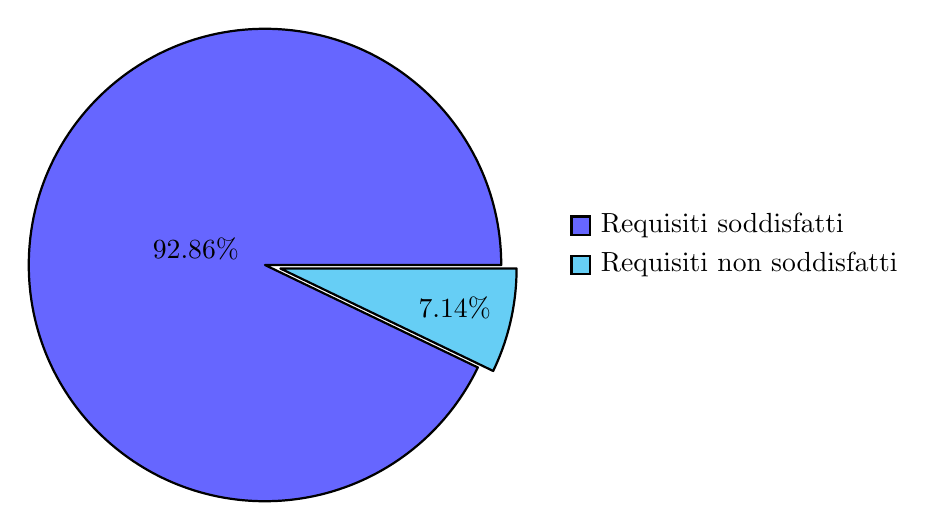
\begin{tikzpicture}
                \pie [explode=0.1, text=legend] { 92.86/Requisiti soddisfatti, 7.14/Requisiti non soddisfatti }
                \end{tikzpicture}
                \caption{Percentuale di soddisfazione dei requisiti funzionali}
        \end{figure}
        \begin{figure}[H]
                \centering
                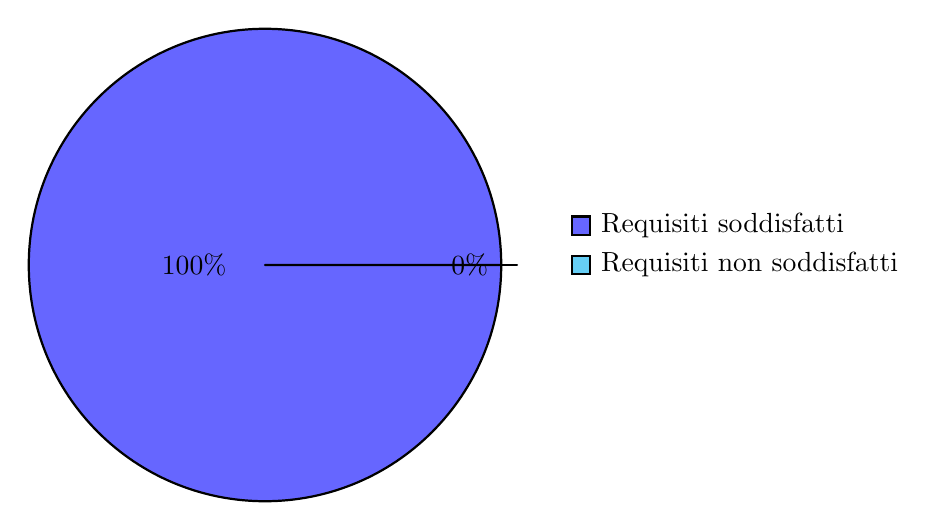
\begin{tikzpicture}
                \pie [explode=0.1, text=legend] { 100/Requisiti soddisfatti, 0/Requisiti non soddisfatti }
                \end{tikzpicture}
                \caption{Percentuale di soddisfazione dei requisiti funzionali obbligatori}
        \end{figure}
        \begin{figure}[H]
                \centering
                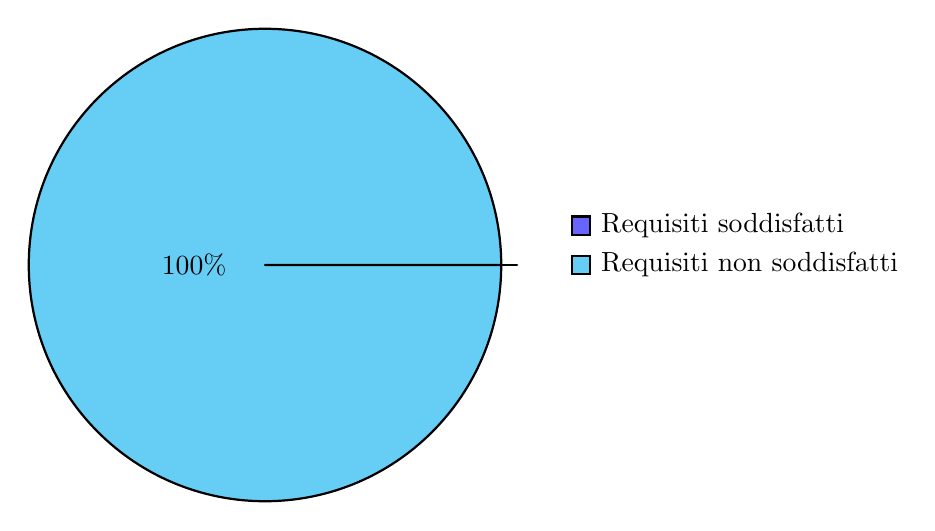
\begin{tikzpicture}
                \pie [explode=0.1, text=legend] { 0/Requisiti soddisfatti, 100/Requisiti non soddisfatti }
                \end{tikzpicture}
                \caption{Percentuale di soddisfazione dei requisiti funzionali opzionali}
        \end{figure}
        \begin{figure}[H]
                \centering
                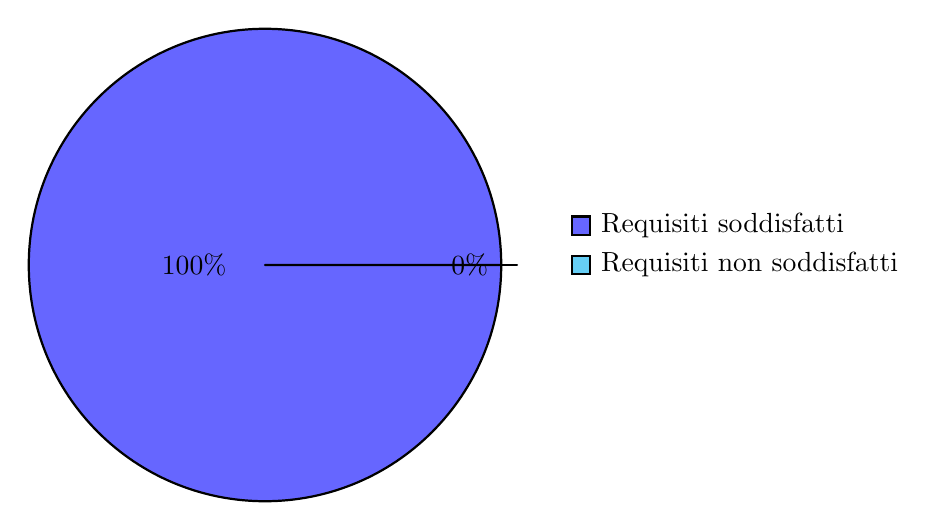
\begin{tikzpicture}
                \pie [explode=0.1, text=legend] { 100/Requisiti soddisfatti, 0/Requisiti non soddisfatti }
                \end{tikzpicture}
                \caption{Percentuale di soddisfazione dei requisiti funzionali desiderabili}
        \end{figure}
    }
\end{document}
